\documentclass[12pt]{article}
\usepackage[margin=1in]{geometry}

% TODO: Create the following new visualizations to enhance research presentation:
% 1. Multi-factor Analysis Chart: Showing interaction between model type, fusion method, and dataset
% 2. Ablation Study Visualization: Demonstrating impact of removing different components
% 3. Error Analysis Heat Map: Showing which emotion pairs are most frequently confused
% 4. Performance vs Complexity Graph: Plotting accuracy against model size/inference time
% 5. Learning Curve Comparison: Showing how different models learn over training epochs
% 6. Feature-Fusion Performance Matrix: A heatmap showing how different audio feature and fusion 
%    strategy combinations perform

% The preceding line only needs to identify funding in the first footnote. If that is unnecessary, please comment on it.
\usepackage{float}
\usepackage[table]{xcolor}
\usepackage{cite}
\usepackage{subcaption}
\usepackage{multirow}
\usepackage{graphicx}
\usepackage{amsmath,amssymb,amsfonts}
\usepackage{algorithmic}
\usepackage{graphicx}
\usepackage{textcomp}
\usepackage{xcolor}
\usepackage{multirow}
\usepackage{setspace}
\usepackage{tabularx}
\usepackage{url}
\usepackage{tabularray}
\usepackage{makecell}
\usepackage{placeins}
\usepackage{comment}
\usepackage{verbatim}
\usepackage{rotating}
\usepackage{changepage}
\renewcommand{\cellalign}{cl}

\usepackage{booktabs, multirow} % for borders and merged ranges
\usepackage{soul}% for underlines
\usepackage[table]{xcolor} % for cell colors
\usepackage{threeparttable} % for wide tables

\usepackage{pdflscape}  % For landscape environment
\usepackage{adjustbox}  % For adjustbox environment

\def\BibTeX{{\rm B\kern-.05em{\sc i\kern-.025em b}\kern-.08em
    T\kern-.1667em\lower.7ex\hbox{E}\kern-.125emX}}
    
    
    \newcommand*{\affaddr}[1]{#1} % No op here. Customize it for different styles.
\newcommand*{\affmark}[1][*]{\textsuperscript{#1}}
\newcommand*{\email}[1]{\textit{#1}}
    
\begin{document}
\begin{center}
\Large
\thispagestyle{empty}

\textbf{Two-Stage Emotion Detection from Multimodal Data}\\
\vspace{0.1in}
\large
\text{A Project Report}\\
\vspace{2in}

\text{Presented to}\\
\text{The Faculty of the Department of Computer Science}\\
\text{San Jose State University}\\

\vspace{1in}

\text{In Partial Fulfillment}\\
\text{of the Requirements for the Degree of}\\
\text{Master of Science}\\

\vspace{1in}

\text{By}\\
\text{Xiangyi Li}\\
\text{Spring 2024}\\

\end{center}

\title{}
\newpage
\thispagestyle{empty}
\begin{center}
\Large
\text{The Designated Project Committee Approves the Project Titled}\\
\vspace{0.1in}
\Large
\text{Two-Stage Emotion Detection from Multimodal Data}\\
\vspace{0.5in}
\text{by}\\
\vspace{0.1in}
\text{Xiangyi Li}\\
\vspace{1.5in}
\Large
\text{APPROVED FOR THE DEPARTMENT OF COMPUTER SCIENCE} \\
\vspace{0.1in}
\text{SAN JOSÉ STATE UNIVERSITY} \\
\vspace{0.1in}
\text{Spring 2024}\\
\vspace{1.5in}
\Large
\begin{tabular}{lcl}
Prof. Faranak Abri & \hspace{1cm} & Department of Computer Science \\
Prof. Fabio Di Troia & \hspace{1cm} & Department of Computer Science \\
Ms. Shuyi Wang & \hspace{1cm} & International Monetary Fund
\end{tabular}
 

\end{center}
\newpage

\pagenumbering{roman}
%\linespread{1.5} 

\doublespacing
\section*{Abstract}
\bigskip
Emotion detection plays a crucial role in human-computer interaction, enabling machines to recognize and respond appropriately to human emotional states. This project explores a two-stage approach to emotion detection using multimodal data, specifically analyzing both textual content and audio features. We investigate different model architectures including transformer-based language models like BERT, RoBERTa, and DeBERTa, alongside various fusion techniques for combining modalities. Using the IEMOCAP dataset in both its complete and filtered versions, we evaluate the effectiveness of single-modality versus multimodal approaches. Our findings demonstrate that transformer-based models, particularly RoBERTa, achieve the highest accuracy when processing textual data alone, while hybrid and late fusion methods yield superior performance when combining text with audio features, particularly MFCC and spectrogram representations. The optimal configuration combines the RoBERTa model with MFCC features using hybrid fusion, achieving an impressive validation accuracy of 91.74\%. This research contributes valuable insights into the relative importance of different modalities and fusion strategies for emotion recognition systems, with potential applications in affective computing, mental health monitoring, and more intuitive human-machine interfaces.\\

\noindent \textbf{Keywords:} Emotion Detection, Natural Language Processing, Multimodal Analysis, Audio Processing, Transformer Models, Fusion Techniques
\newpage
%-------------------------------------------------------------------------------------------------
\section*{Acknowledgements}
I would like to express my sincere gratitude to my advisor, Professor Faranak Abri, for her invaluable guidance and support throughout this project. Her insights and feedback have helped me navigate challenges and achieve my goals. Thank you for your mentorship and encouragement.\\
  
\noindent
I would like to extend my gratitude to all members of my defense committee, Professor Fabio Di Troia, and Ms. Shuyi Wang.\\

\noindent  
I would like to extend my heartfelt thanks to my family and friends for their unwavering support and encouragement throughout my academic journey and in all aspects of my life.

\bigskip

\newpage
\tableofcontents
\newpage
\bigskip
\listoffigures
\listoftables


\newpage
\vspace{-0.1in}
\pagenumbering{arabic}
\section{Introduction}
\label{sec:intro}
Emotion recognition plays a fundamental role in human communication, allowing us to understand others' feelings, intentions, and needs. As artificial intelligence systems become increasingly integrated into our daily lives, the ability for machines to recognize and respond appropriately to human emotions has become crucial for meaningful human-computer interaction. This capability, often referred to as affective computing, has applications ranging from healthcare and education to entertainment and customer service.

Emotions are expressed through multiple channels, including facial expressions, voice modulations, body language, and verbal content. While humans naturally process these cues simultaneously to gauge emotional states, developing computational systems that can effectively interpret and integrate these diverse signals remains challenging. Traditional approaches often focus on a single modality, such as analyzing facial expressions or processing textual content, which limits their robustness across different contexts.

The challenge in emotion detection stems from several factors. First, emotions are inherently subjective and exist on a spectrum rather than as discrete categories. Second, emotional expressions vary considerably across individuals, cultures, and contexts. Third, different modalities may convey conflicting emotional information, requiring sophisticated fusion techniques to resolve inconsistencies. Furthermore, environmental factors like background noise or lighting conditions can significantly impact the quality of input signals.

To address these challenges, this project explores a two-stage approach to emotion detection using multimodal data. The first stage involves processing individual modalities—specifically text and audio features—through specialized models tailored to each data type. The second stage employs various fusion techniques to combine these modality-specific representations, leveraging their complementary strengths while mitigating their individual weaknesses.

Our research makes several key contributions:

\begin{enumerate}
    \item Comparative Analysis of Language Models: We evaluate the performance of various transformer-based models, including BERT, RoBERTa, XLNet, ALBERT, ELECTRA, and DeBERTa, for textual emotion recognition.
    
    \item Audio Feature Exploration: We investigate the effectiveness of different audio representations, including Mel-Frequency Cepstral Coefficients (MFCC), spectrograms, prosodic features, and wav2vec embeddings.
    
    \item Fusion Strategy Assessment: We systematically compare early, late, hybrid, and attention-based fusion approaches for integrating textual and audio modalities.
    
    \item Benchmark Dataset Evaluation: We conduct experiments on both the complete and filtered versions of the IEMOCAP dataset, providing insights into the impact of data preprocessing on model performance.
    
    \item Modal Cloud Infrastructure: We implement a scalable and reproducible experimental framework using Modal's cloud infrastructure, enabling efficient parallel execution of numerous experiments.
\end{enumerate}

The structure of this report is as follows: Section \ref{sec:related} reviews relevant literature on emotion recognition approaches. Section \ref{sec:methodology} describes our methodology, including model architectures and fusion strategies. Section \ref{sec:experimental_setup} details the experimental setup, covering dataset preparation, preprocessing techniques, and evaluation metrics. Section \ref{sec:results} presents our findings, while Section \ref{sec:discussion} discusses their implications. Finally, Section \ref{sec:conclusion} concludes the report and suggests directions for future research.

\section{Related Work}
\label{sec:related_work}

\subsection{Early Emotion-Recognition Approaches (pre-2012)}
The first wave of emotion-recognition (ER) research was dominated by
lexicon and rule-based techniques such as WordNet-Affect
\cite{strapparava2004wordnet} and the NRC Emotion Lexicon
\cite{mohammad2013nrc}.  Classical machine-learning models—Naïve Bayes,
logistic regression and \textsc{svm}—were trained on bag-of-words, TF–IDF
or \textsc{liwc} counts for text ER, and on low-level descriptors for
speech or facial data \cite{schuller2009acoustic}.  These systems rarely
exceeded $\approx$60 \% accuracy on early benchmarks and were brittle to
contextual nuance.

\subsection{Deep-Learning Era (2013–2017)}
Convolutional and recurrent networks rapidly eclipsed classical models.
CNNs and \mbox{(Bi-)LSTMs} learned richer semantic and temporal features
for text, audio and vision.  In speech ER, CNN-style spectrogram
encoders combined with LSTM temporal heads pushed performance above
90 \% on Emo-DB and IEMOCAP \cite{mao2014learning}.  Hybrid CNN-LSTM
architectures similarly boosted textual ER
\cite{abdul2017emonet}.  Multimodal early-fusion CNNs that concatenate
openSMILE prosody, word embeddings and 3-D CNN facial features achieved
$\approx$80 \% on CMU-MOSI \cite{poria2018multimodal}.  Although
effective, these networks struggled with asynchronous modalities and
long-range context.

\subsection{Transformer-Based Models (2018–2025)}
Contextualised language models revolutionised unimodal ER.  Fine-tuning
BERT, RoBERTa or DeBERTa yields state-of-the-art textual accuracies on
many datasets \cite{liu2019roberta}.  Cross-modal transformers extend
self-attention to heterogeneous streams.  \textsc{MulT}
\cite{tsai2019mult} attends across mis-aligned audio, visual and
linguistic tokens, attaining 84.8 \% unweighted accuracy (UA) on the
six-class IEMOCAP task.  Progressive-modality reinforcement
\cite{lv2021progressive} iteratively re-weights modalities, while
TransModality \cite{wang2020context} unifies feature extraction and
fusion within one transformer backbone.  Self-supervised encoders such
as Wav2Vec 2.0 supply powerful speech features that, when fused with
RoBERTa text embeddings, reach 84.7 \% UA on IEMOCAP and 64 \% F1 on the
challenging MELD corpus \cite{siriwardhana2020joint}.

\subsection{Multimodal Fusion Taxonomy}
Fusion strategies fall into three categories:

\textbf{Early fusion} concatenates raw features before a shared
classifier \cite{poria2017review}.  It captures low-level correlations
but ignores modality structure.

\textbf{Late fusion} trains modality-specific classifiers whose logits
are fused by averaging or a meta-learner
\cite{wang2019words}.  Flexibility is high, yet fine-grained
interactions are lost.

\textbf{Hybrid / fine-grained fusion} combines both.  Tensor Fusion
Networks \cite{zadeh2018multimodal_tfn}, Memory Fusion Networks
\cite{zadeh2018mfn}, capsule-based interaction
\cite{wang2019words} and cross-modal transformers
\cite{tsai2019mult} explicitly model inter-modal dynamics and achieve
the best overall results (e.g., 89 \% accuracy on CMU-MOSEI
\cite{mittal2020m3er}).

\subsection{Benchmark Datasets}
\textbf{IEMOCAP} \cite{busso2008iemocap} remains the de-facto benchmark
($\sim$10 k utterances, 9 emotions, audio+video+transcripts).  
\textbf{CMU-MOSI} \cite{zadeh2016mosi} and
\textbf{CMU-MOSEI} \cite{zadeh2018multimodal} provide large
"in-the-wild'' video reviews with sentiment and six-emotion labels.
\textbf{MELD} \cite{poria2018meld} introduces multi-party dialogue
context; \textbf{RAVDESS} \cite{livingstone2018ravdess} supplies
balanced acted speech.  Each poses distinct challenges in spontaneity,
noise and class imbalance, motivating the use of unweighted metrics
(UAR, UF1) alongside accuracy and weighted F1.

\subsection{Current Challenges}
Despite progress, open problems persist: domain shift (lab $\rightarrow$
wild) causes 15–20 pp degradation; demographic bias is under-studied;
conversation-level understanding and real-time, low-resource deployment
remain difficult.  Addressing these issues requires larger,
diversified corpora and efficient, bias-aware models.

\clearpage
\begin{table}[p]
\sffamily\tiny
\centering
\caption{Comparison of Emotion Detection Models (Multimodal, Text, Audio)}
\renewcommand{\arraystretch}{0.85}
\setlength{\tabcolsep}{1.8pt}
\begin{adjustbox}{width=\textwidth,center}
\begin{tabular}{@{}p{2.3cm}p{1.6cm}p{1.2cm}p{2.4cm}p{2.3cm}p{1.1cm}p{2.1cm}@{}}
\toprule
\textbf{Reference} & \textbf{Dataset} & \textbf{Modality} & \textbf{Features} & \textbf{Classification} & \textbf{Metric} & \textbf{Performance} \\
\midrule
Poria et al. (2017) & CMU-MOSI (binary) & S+T+V & openSMILE, word2vec, 3D-CNN & Early fusion (feature concat) & Acc & 81.3\% \\
Liu et al. (2018) & IEMOCAP (4) & S+T+V & COVAREP, GloVe, FACET & Utterance interaction (memory) & UF1 & 83.1\% \\
Zadeh et al. (2018) & YT(3), MOUD(2), IEMOCAP(9) & S+T+V & COVAREP, GloVe, FACET & Fine-grained interaction (tensor) & Acc/F1 & YT: 61.0\%/60.7\%; MOUD: 81.1\%/80.4\%; IEMO: 36.5\%/34.9\% \\
Pham et al. (2019) & CMU-MOSI (binary) & S+T+V & MFCC, GloVe, FACET+OpenFace & Fine-grained interaction & Acc/F1 & 76.5\%/73.4\% \\
Poria et al. (2018) & IEMOCAP(4), MOUD(2), MOSI(2) & S+T+V & openSMILE, CNN, 3D-CNN & Early fusion (multimodal CNN) & Acc & IEMO: 71.6\%; MOUD: 67.9\%; MOSI: 76.7\% \\
Zadeh et al. (2018) & CMU-MOSEI (6) & S+T+V & COVAREP, GloVe, MTCNN & Fine-grained (dynamic fusion) & UAcc/UF1 & 62.4\%/76.3\% \\
Majumder et al. (2018) & MOSI(2), IEMOCAP(4) & S+T+V & openSMILE, word2vec, 3D-CNN & Hierarchical fusion w/ context & Acc & MOSI: 80.0\%; IEMO: 76.5\% \\
Tsai et al. (2019) & ICT-MMMO(2), YT(3), MOUD(2), IEMOCAP(6) & S+T+V & COVAREP, GloVe, FACET & Cross-modal Transformer (MULT) & Acc/F1 & ICT: 81.3\%/79.2\%; YT: 53.3\%/52.4\%; MOUD: 82.1\%/81.7\%; IEMO: 84.8\%(UAcc)/81.4\%(UF1) \\
Wang et al. (2019) & IEMOCAP (4) & S+T+V & COVAREP, GloVe, FACET & Fine-grained (Capsule network) & UAcc/UF1 & 81.9\%/81.2\% \\
Tsai et al. (2018) & IEMOCAP (4) & S+T+V & COVAREP, GloVe, FACET & Factorized multimodal rep. & UAcc/UF1 & 74.7\%/71.5\% \\
Pham et al. (2020) & ICT-MMMO(2), YT(2) & S+T+V & COVAREP, GloVe, FACET & Fine-grained interaction & Acc/F1 & ICT: 81.3\%/80.8\%; YT: 51.7\%/52.4\% \\
Liang et al. (2021) & IEMOCAP(4), MELD(7) & S+T+V & openSMILE, BERT, DenseNet & Simple feature concat & Acc/F1 & IEMO: 75.6\%(UAcc 74.5\%); MELD: 57.1\%(F1) \\
Mittal et al. (2021) & IEMOCAP(4), MOSEI(6) & S+T+V & MFCC/pitch, GloVe, facial AUs & Fine-grained (CNN+LSTM) & Acc/F1 & IEMO: 82.7\%/82.4\%; MOSEI: 89.0\%/80.2\% \\
Wang et al. (2020) & IEMOCAP(6), MOSI(2), MELD(7) & S+T+V & openSMILE, CNN, 3D-CNN & End-to-end Transformer & Acc & IEMO: 60.8\%; MELD: 62.0\%; MOSI: 82.7\% \\
Sun et al. (2020) & IEMOCAP (4) & S+T+V & COVAREP, BERT, FACET & Deep CCA (correlation) & UAcc/UF1 & 83.0\%/81.8\% \\
Siriwardhana (2020) & IEMOCAP(4), MELD(7) & S+T+V & Wav2Vec, RoBERTa, FabNet & Transformer-based late fusion & UAcc/F1 & IEMO: 84.7\%/84.2\%; MELD: 64.3\%/63.9\% \\
Lv et al. (2021) & IEMOCAP(4), MOSI(2) & S+T+V & COVAREP, BERT, FACET & Progressive modality reinforce & UAcc/UF1 & IEMO: 85.1\%/83.8\%; MOSI: 83.6\%/83.4\% \\
Majumder et al. (2019) & MELD (7) & T(conv) & GloVe, context state & GRU-based RNN (party-state) & WF1 & 57.0\% \\
Ghosal et al. (2019) & MELD (7) & T(conv) & GloVe, speaker depend. & Graph convolution network & WF1 & 58.1\% \\
Ghosal et al. (2020) & MELD (7) & T(conv) & RoBERTa, commonsense & Transformer + commonsense & WF1 & 65.2\% \\
Trinh et al. (2022) & IEMOCAP (4) & A & Mel spectrogram, spectral feat. & CNN + GRU (ensemble) & Acc & 97.47\% \\
Issa et al. (2020) & RAVDESS (8) & A & MFCC, spectral contrast, mel-spec & Deep NN (fully-connected) & Acc & 71.6\% \\
Bautista et al. (2021) & RAVDESS (8) & A & Augmented spectrograms & Parallel CNN–Transformer & Acc & 89.33\% \\
Pan et al. (2022) & IEMOCAP (4) & A & MFCC features & CNN + LSTM hybrid & Acc & 96.21\% \\
\bottomrule
\end{tabular}
\end{adjustbox}
\vspace{1mm}
\begin{flushleft}
{\tiny Note: S=Speech, T=Text, V=Visual, A=Audio, Acc=Accuracy, UF1=Unweighted F1, WF1=Weighted F1, YT=YouTube, IEMO=IEMOCAP}
\end{flushleft}
\end{table}
\clearpage

\subsection{Audio-Based Emotion Detection}
Audio-based emotion recognition has traditionally focused on extracting acoustic features that correlate with emotional states. Low-level descriptors (LLDs) such as pitch, energy, formants, and voice quality parameters were among the earliest features explored~\cite{schuller2009acoustic}.

Mel-Frequency Cepstral Coefficients (MFCCs), originally developed for speech recognition, have proven effective for emotion detection by capturing the spectral envelope of speech~\cite{li2013speech}. Similarly, spectrograms provide time-frequency representations that preserve temporal dynamics important for emotion recognition.

With deep learning, Convolutional Neural Networks (CNNs) have been applied directly to spectrograms, treating them as images and learning relevant patterns automatically~\cite{mao2014learning}. This approach eliminates the need for handcrafted feature engineering while often improving performance.

More recently, self-supervised approaches like wav2vec~\cite{schneider2019wav2vec} have gained attention by learning representations from unlabeled audio data. These models capture nuanced acoustic properties that may be missed by traditional feature extraction methods.

\subsection{Multimodal Approaches}
Recognizing that emotions are expressed through multiple channels, researchers have increasingly focused on multimodal approaches. These methods face the challenge of effectively combining information from different modalities that may operate at different time scales and granularities.

Early fusion (feature-level) combines raw features or low-level representations before classification, allowing the model to learn joint patterns across modalities~\cite{poria2017review}. While conceptually simple, this approach must handle different feature dimensions and time scales.

Late fusion (decision-level) processes each modality independently and combines their predictions, typically through voting schemes, weighted averaging, or additional classifiers~\cite{wagner2011introducting}. This approach is more modular but may miss cross-modal interactions.

Hybrid fusion combines aspects of both early and late fusion, often using attention mechanisms to dynamically weight different modalities based on their relevance~\cite{zadeh2018memory}. These approaches have shown promising results by adapting to varying reliability of modalities across different inputs.

Transformer-based models have recently been extended to the multimodal domain, with architectures like MMBT~\cite{kiela2019supervised} jointly encoding textual and visual information. These approaches leverage the self-attention mechanism to capture relationships both within and across modalities.

\subsection{Emotion Recognition Datasets}
Several benchmark datasets have been developed for emotion recognition research. The Interactive Emotional Dyadic Motion Capture (IEMOCAP) dataset~\cite{busso2008iemocap} contains audio-visual recordings of acted dialogues, annotated for categorical emotions and dimensional affect labels. It has become one of the most widely used resources for multimodal emotion recognition.

Other notable datasets include SEMAINE~\cite{mckeown2012semaine}, which features interactions between humans and artificially intelligent agents; RAVDESS~\cite{livingstone2018ryerson}, containing emotional speech and song; and CMU-MOSEI~\cite{zadeh2018multimodal}, which includes YouTube video clips with sentiment and emotion annotations.

Our work builds upon these foundations by systematically comparing state-of-the-art transformer models for text processing, exploring various audio feature representations, and evaluating different fusion strategies on the IEMOCAP dataset.

\section{Methodology}
\label{sec:methodology}
Our approach to emotion detection employs a two-stage architecture that processes textual and audio modalities separately before combining them through various fusion strategies. This section provides a comprehensive overview of our methodology, including detailed descriptions of model architectures, audio feature extraction techniques, training procedures, and fusion methods.

\subsection{System Architecture Overview}
Figure~\ref{fig:system_architecture} illustrates the high-level architecture of our two-stage emotion detection system. The first stage consists of separate processing pipelines for textual and audio data, each optimized for the specific characteristics of its modality. The second stage implements various fusion strategies to combine information from both modalities for the final emotion classification.

\begin{figure}[h]
    \centering
    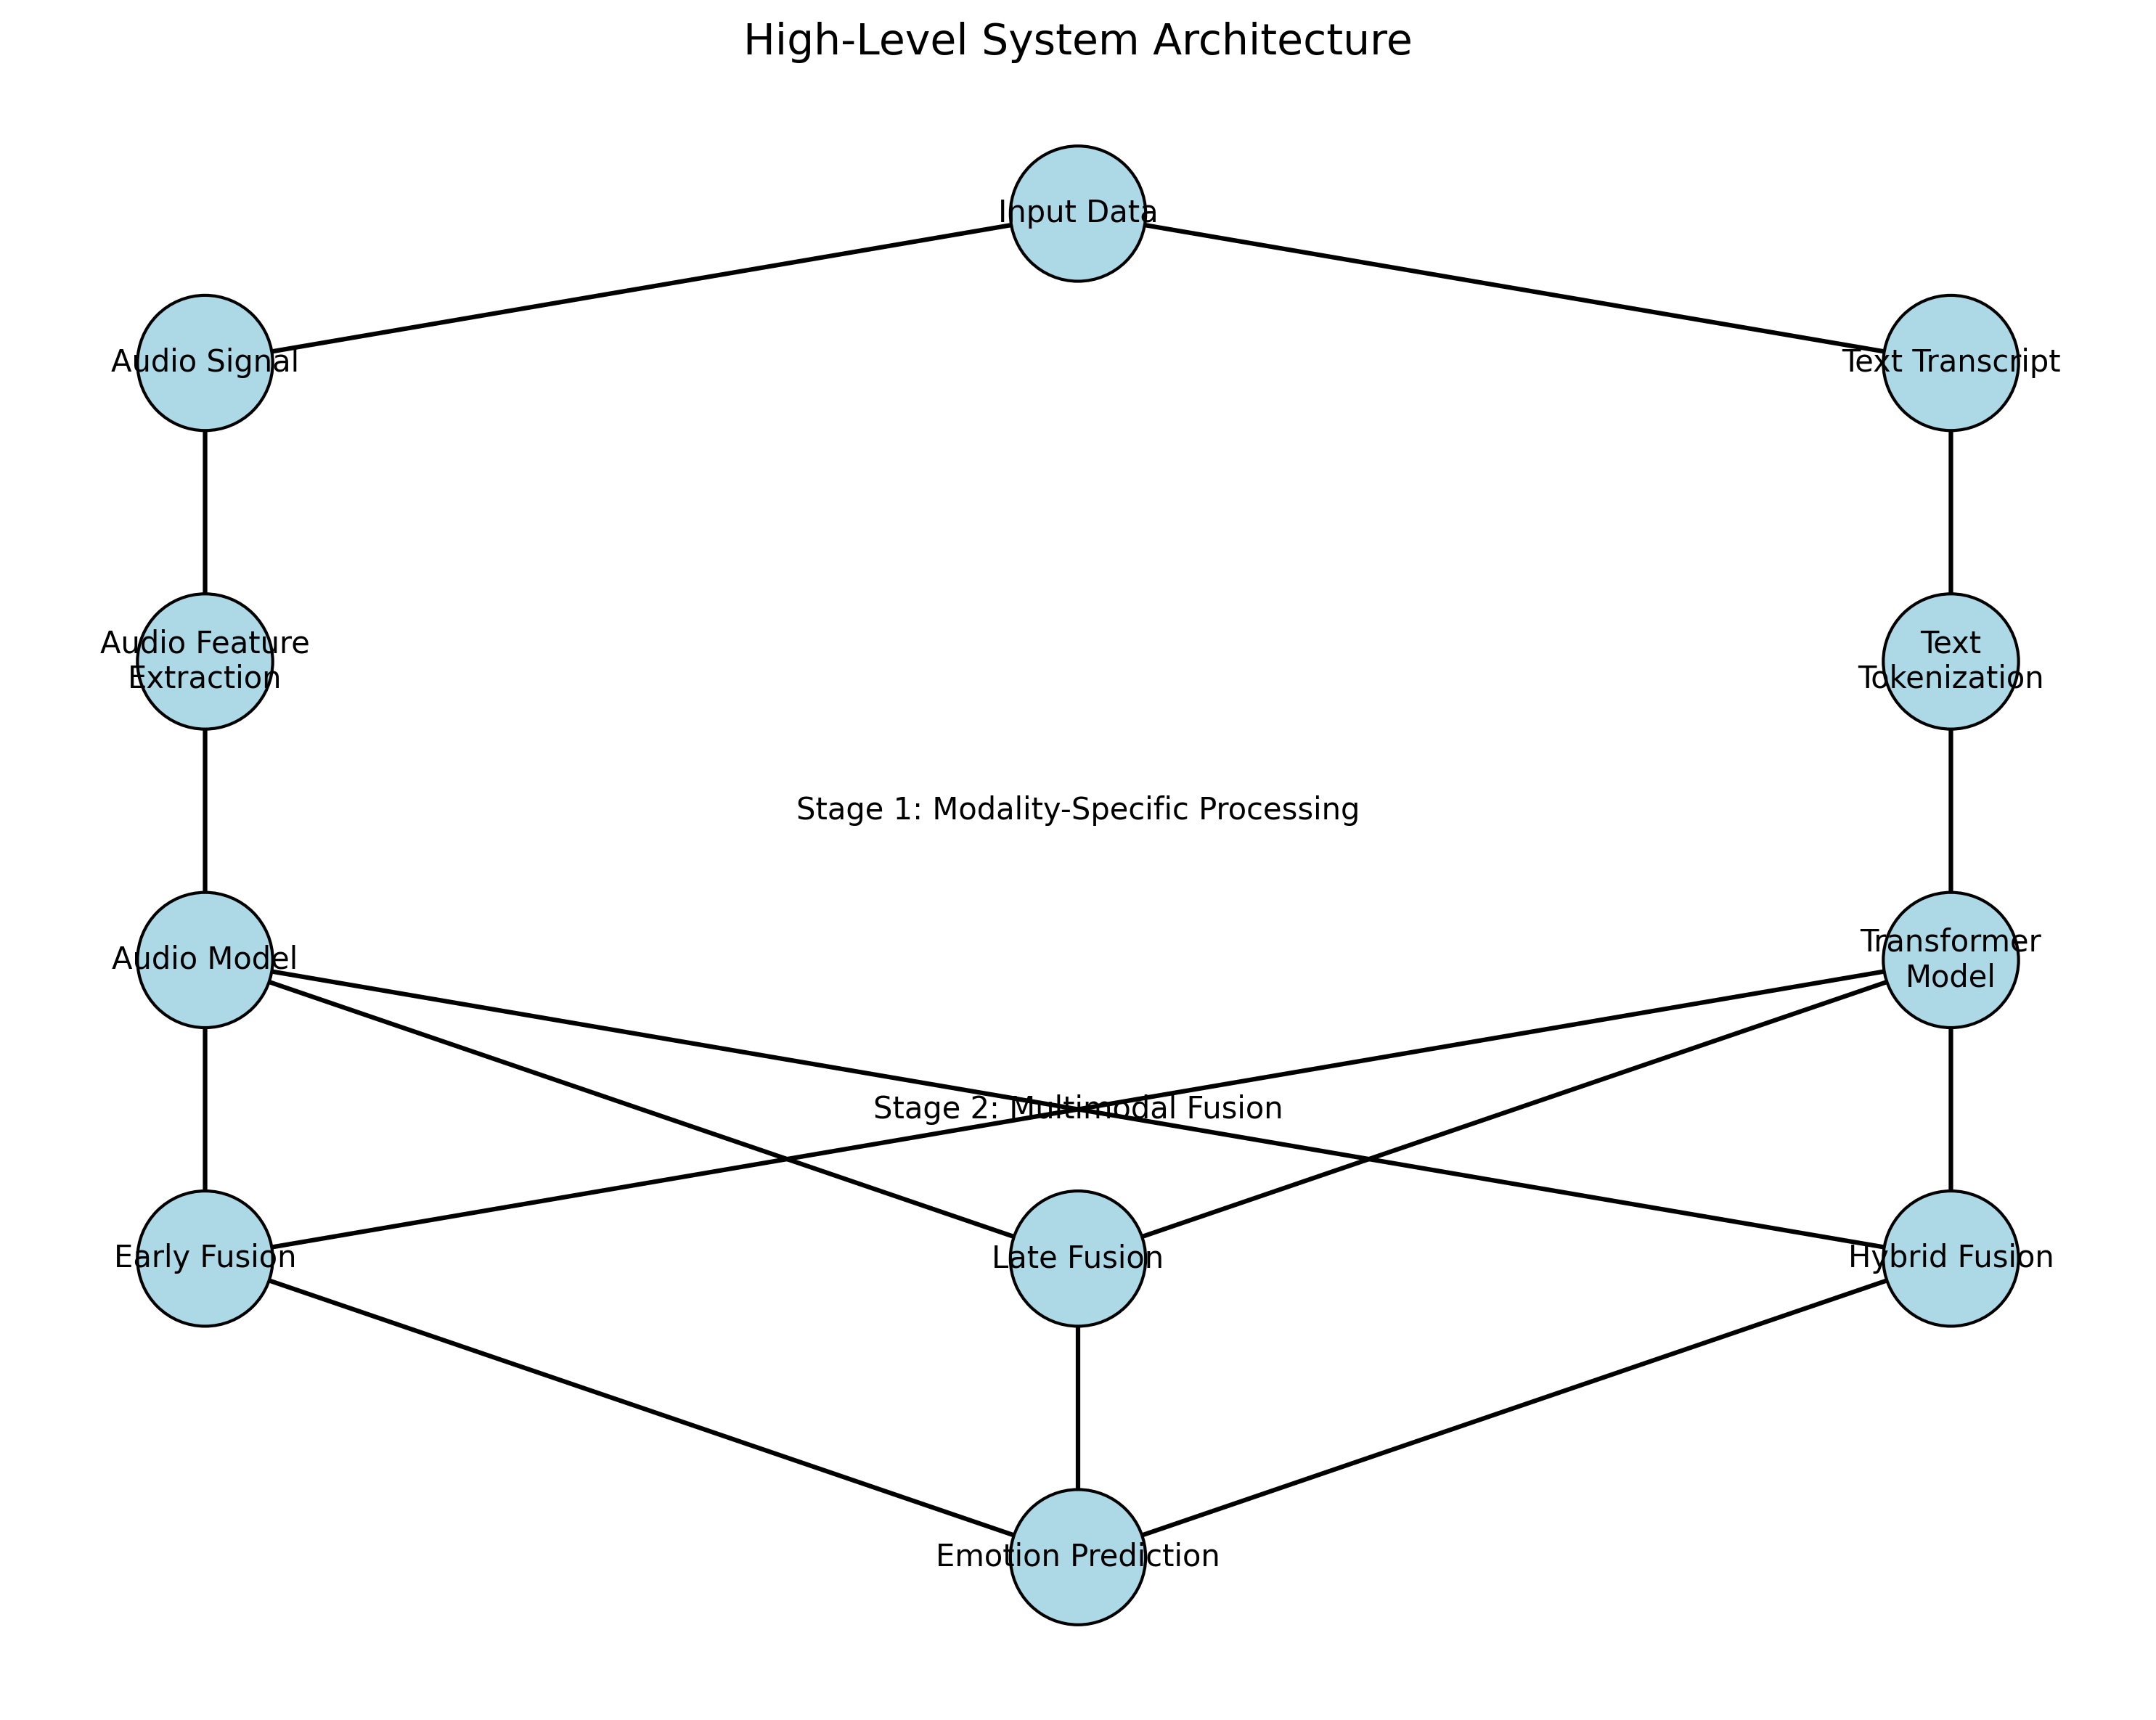
\includegraphics[width=0.9\linewidth]{Figures/system_architecture_fixed.png}
    \caption{High-Level System Architecture: The diagram illustrates the two-stage approach with modality-specific processing of audio and text followed by multimodal fusion strategies. Showing the complete data flow from input processing through emotion prediction, this architectural overview highlights the parallel processing streams and fusion options implemented in our system.}
    \label{fig:system_architecture}
\end{figure}

This modular design offers several advantages:
\begin{itemize}
    \item It allows for independent optimization of each modality's processing pipeline
    \item It facilitates experimentation with different combinations of models and fusion strategies
    \item It provides flexibility to handle missing modalities by falling back to single-modality predictions
    \item It enables better interpretability through analysis of each modality's contribution
\end{itemize}

\subsection{Text Processing Models}
For processing textual data, we evaluated several state-of-the-art transformer-based models. Each model was implemented using the Hugging Face Transformers library, with a classification head added on top of the base model for emotion recognition.

\subsubsection{BERT (Bidirectional Encoder Representations from Transformers)}
BERT~\cite{devlin2018bert} revolutionized NLP by introducing bidirectional context modeling through a masked language modeling objective. The model architecture consists of multiple transformer encoder layers that process tokens in parallel, with each token attending to all other tokens in the sequence.

\paragraph{Architecture Details:}
\begin{itemize}
    \item Variant: bert-base-uncased
    \item Layers: 12 transformer encoder layers
    \item Hidden size: 768 dimensions
    \item Attention heads: 12
    \item Parameters: 110 million
    \item Maximum sequence length: 512 tokens
    \item Vocabulary size: 30,522 tokens
\end{itemize}

\paragraph{Pre-training Objectives:}
\begin{itemize}
    \item Masked Language Modeling (MLM): Randomly mask 15\% of input tokens and predict them based on bidirectional context
    \item Next Sentence Prediction (NSP): Predict whether two sentences appear consecutively in the original text
\end{itemize}

\paragraph{Fine-tuning Approach:}
For emotion classification, we extracted the final hidden state of the [CLS] token, which serves as an aggregate representation of the entire input sequence. This representation was passed through a classification layer with a single hidden layer of 768 units and ReLU activation, followed by a softmax output layer with the number of units matching the number of emotion categories.

\subsubsection{RoBERTa (Robustly Optimized BERT Approach)}
RoBERTa~\cite{liu2019roberta} builds upon BERT with several optimizations to the training methodology. It maintains the same architecture but eliminates the next sentence prediction objective, uses dynamic masking patterns, longer sequences, and larger batch sizes.

\paragraph{Architectural Improvements:}
\begin{itemize}
    \item Variant: roberta-base
    \item Same architecture as BERT (12 layers, 768 hidden size, 12 attention heads)
    \item Vocabulary size: 50,265 tokens (using byte-level BPE)
    \item Parameters: 125 million
\end{itemize}

\paragraph{Training Enhancements:}
\begin{itemize}
    \item Removal of Next Sentence Prediction task
    \item Dynamic masking: Creates new masking patterns each time a sequence is presented to the model
    \item Larger batch sizes: Trained with batch sizes of 8K sequences
    \item More data: Pre-trained on 160GB of text versus BERT's 16GB
    \item Longer training: Trained for more steps with larger batches
\end{itemize}

\paragraph{Implementation Details:}
Our RoBERTa implementation used the RobertaForSequenceClassification class from the Transformers library, which adds a classification head on top of the RoBERTa encoder. We initialized this model with pre-trained weights and fine-tuned all layers during training.

\subsubsection{XLNet}
XLNet~\cite{yang2019xlnet} introduces a generalized autoregressive pre-training method that captures bidirectional context while avoiding BERT's assumption of independence between masked tokens.

\paragraph{Key Innovations:}
\begin{itemize}
    \item Permutation Language Modeling: Predicts tokens in random order, learning bidirectional context without independence assumptions
    \item Two-Stream Self-Attention: Uses query stream and content stream to prevent target information leakage
    \item Variant: xlnet-base-cased
    \item Layers: 12 transformer layers
    \item Hidden size: 768 dimensions
    \item Attention heads: 12
    \item Parameters: 110 million
\end{itemize}

\paragraph{Implementation Details:}
For our experiments, we employed the XLNetForSequenceClassification model. The fine-tuning process maintained the same hyperparameters as our BERT and RoBERTa implementations to ensure fair comparison.

\subsubsection{ALBERT (A Lite BERT)}
ALBERT~\cite{lan2019albert} addresses BERT's parameter inefficiency through parameter-reduction techniques while maintaining performance.

\paragraph{Parameter Reduction Techniques:}
\begin{itemize}
    \item Factorized embedding parameterization: Decomposes the large vocabulary embedding matrix into two smaller matrices
    \item Cross-layer parameter sharing: Uses the same parameters for all transformer layers
    \item Variant: albert-base-v2
    \item Layers: 12 transformer layers
    \item Hidden size: 768 dimensions
    \item Parameters: 12 million (approximately 10\% of BERT-base)
\end{itemize}

\paragraph{Additional Improvements:}
\begin{itemize}
    \item Sentence Order Prediction (SOP): Replaces Next Sentence Prediction with a more challenging task of determining if two consecutive segments are in the correct order
    \item Dropout rate of 0 on the embedding layer
\end{itemize}

\subsubsection{ELECTRA (Efficiently Learning an Encoder that Classifies Token Replacements Accurately)}
ELECTRA~\cite{clark2020electra} introduces a more sample-efficient pre-training approach with a replaced token detection objective.

\paragraph{Novel Pre-training Approach:}
\begin{itemize}
    \item Generator-Discriminator architecture: A small generator model (like BERT) produces replacements for masked tokens
    \item Replaced Token Detection: The discriminator learns to classify each token as either "original" or "replaced"
    \item Variant: google/electra-base-discriminator
    \item Layers: 12 transformer layers
    \item Hidden size: 768 dimensions
    \item Parameters: 110 million
\end{itemize}

\paragraph{Advantages:}
\begin{itemize}
    \item More efficient learning: All tokens contribute to the loss, not just the masked ones
    \item Stronger representations: Learning to distinguish subtle differences between real and fake tokens
    \item Faster convergence: Requires less pre-training time for comparable performance
\end{itemize}

\subsubsection{DeBERTa (Decoding-enhanced BERT with disentangled attention)}
DeBERTa~\cite{he2020deberta} enhances BERT with disentangled attention and an enhanced mask decoder.

\paragraph{Key Innovations:}
\begin{itemize}
    \item Disentangled attention: Computes attention weights using two vectors for each word—content and position—instead of one
    \item Enhanced mask decoder: Incorporates absolute positions in the decoding layer
    \item Variant: microsoft/deberta-v3-base
    \item Layers: 12 transformer layers
    \item Hidden size: 768 dimensions
    \item Parameters: 184 million
\end{itemize}

\paragraph{Implementation Details:}
We used the DebertaV2ForSequenceClassification model from the Transformers library, which incorporates the improvements of DeBERTa v3, including better position encoding and a new vocabulary.

\subsubsection{Transformer Architecture Details}
The detailed internal architecture of transformer-based models is critical to understanding their performance characteristics. Figure~\ref{fig:text_model_architecture} illustrates the common components found in the transformer encoder architectures used in our experiments.

\begin{figure}[h]
    \centering
    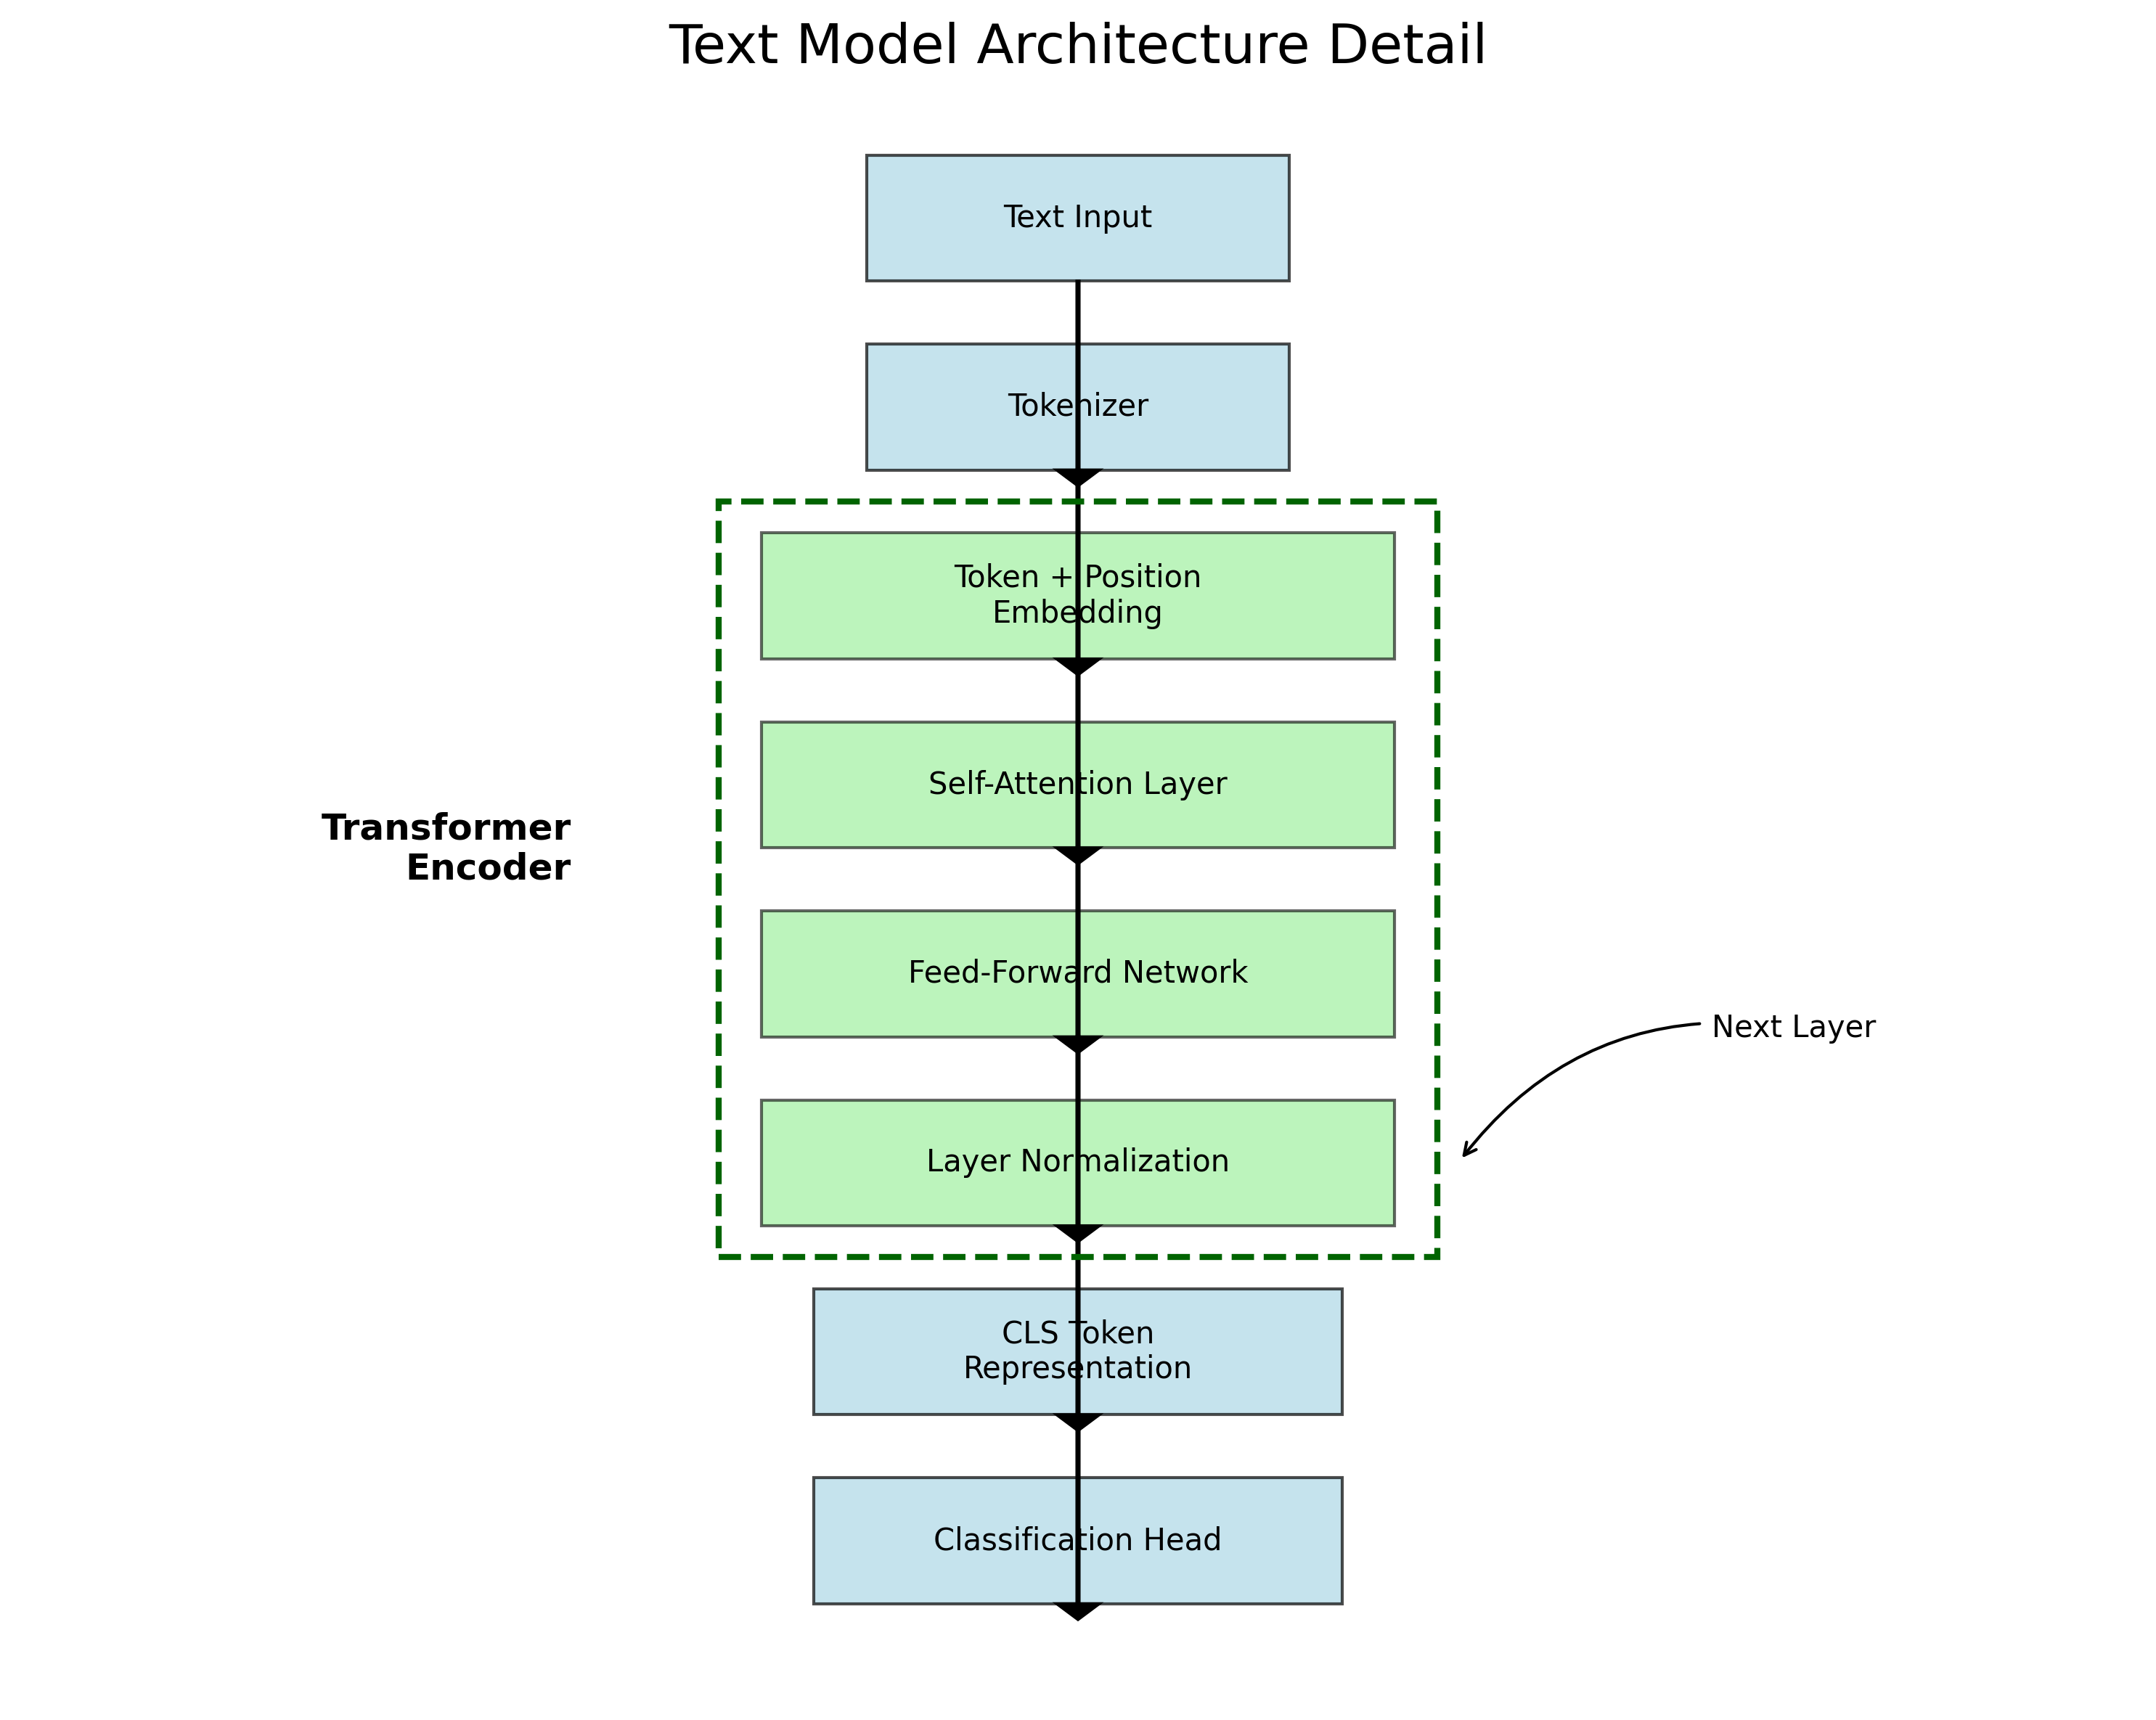
\includegraphics[width=0.85\linewidth]{Figures/text_model_architecture.png}
    \caption{Text Model Architecture Detail: This diagram shows the internal structure of transformer-based models used in our experiments. Starting with tokenization and embedding layers, the architecture features multi-head self-attention mechanisms and feed-forward networks with layer normalization. The CLS token representation from the final layer serves as input to the classification head for emotion prediction.}
    \label{fig:text_model_architecture}
\end{figure}

\subsection{Text Model Training Procedure}
All transformer models followed a consistent training procedure to ensure fair comparison:

\paragraph{Preprocessing:}
\begin{enumerate}
    \item Tokenization using model-specific tokenizers
    \item Truncation/padding to a maximum sequence length of 128 tokens
    \item Creation of attention masks to differentiate between actual tokens and padding
\end{enumerate}

\paragraph{Hyperparameters:}
\begin{itemize}
    \item Learning rate: 2e-5 with linear decay
    \item Batch size: 16 samples
    \item Training epochs: 40 (with early stopping based on validation loss)
    \item Optimizer: AdamW with weight decay of 0.01
    \item Gradient clipping: Maximum gradient norm of 1.0
    \item Warmup: 10\% of total training steps
\end{itemize}

\paragraph{Regularization Techniques:}
\begin{itemize}
    \item Early stopping: Training halted when validation loss failed to improve for 5 consecutive epochs
    \item Dropout: Default dropout rate of 0.1 in transformer layers
    \item Weight decay: Applied to all parameters except biases and layer normalization
\end{itemize}

\paragraph{Loss Function:}
For discrete emotion categories, we used cross-entropy loss. For dimensional emotion recognition (valence, arousal, dominance), we employed mean squared error (MSE) loss.

\subsection{Audio Feature Extraction}
The audio modality provides crucial information about emotional states through prosodic patterns, voice quality, and spectral characteristics. We explored four different audio representation techniques, each capturing different aspects of the speech signal.

\subsubsection{Mel-Frequency Cepstral Coefficients (MFCCs)}
MFCCs are perceptually motivated spectral features that represent the short-term power spectrum of sound, mimicking the human auditory system's frequency response.

\begin{figure}[h]
    \centering
    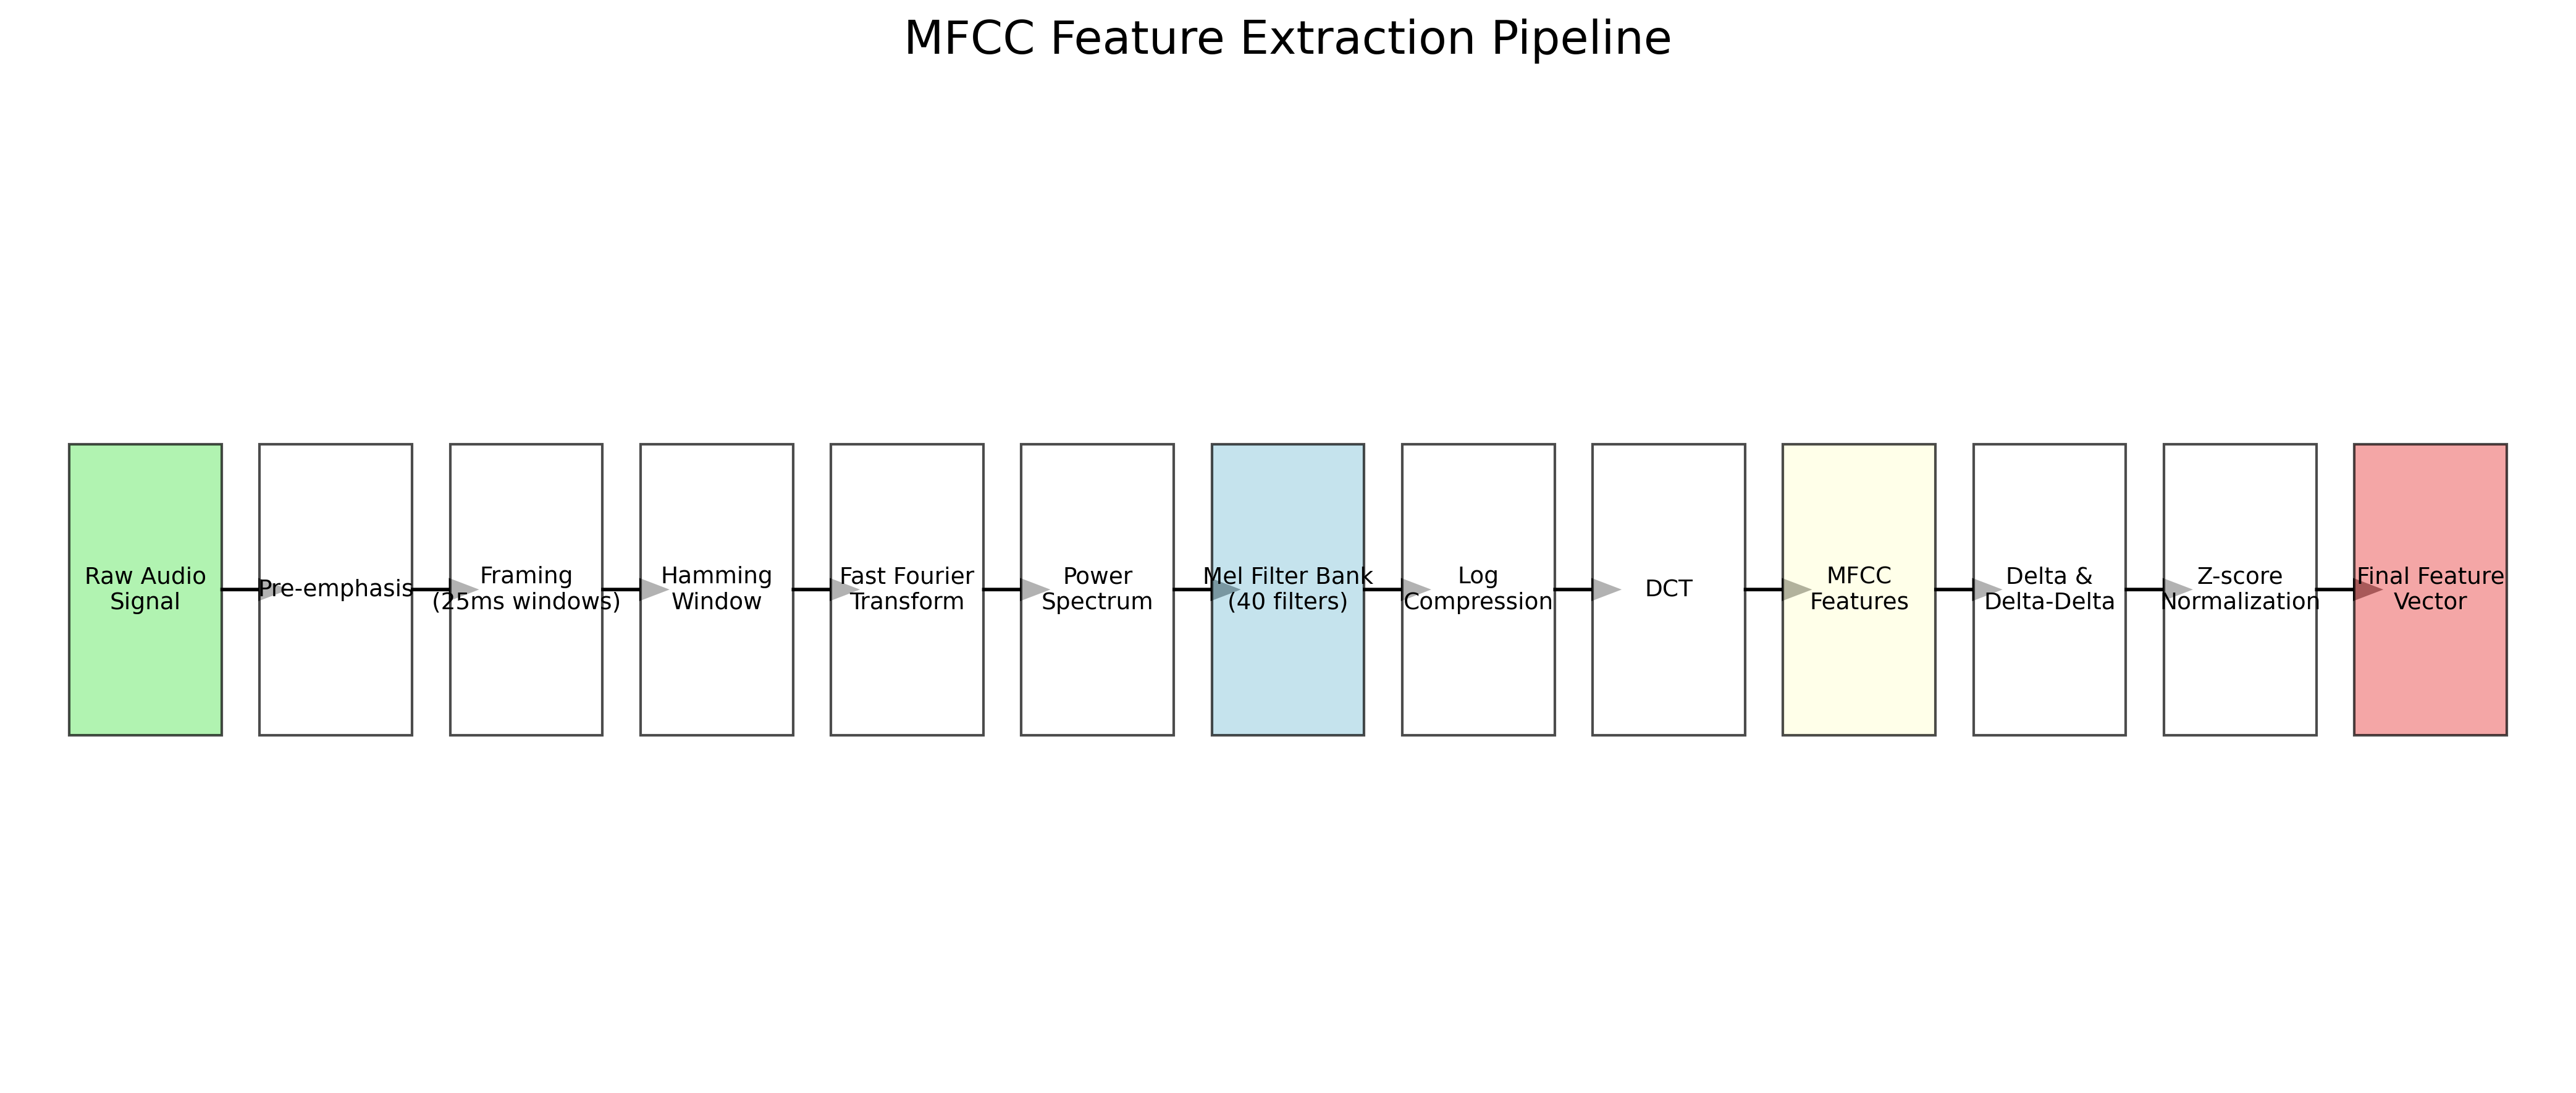
\includegraphics[width=1.0\linewidth]{Figures/mfcc_pipeline.png}
    \caption{MFCC Feature Extraction Pipeline: This diagram details the complete processing pipeline for extracting Mel-frequency cepstral coefficients from raw audio signals. Starting with pre-emphasis and framing, the pipeline applies a series of transformations including FFT, Mel-scale filtering, and DCT to capture perceptually relevant acoustic features. The final feature vector includes delta and delta-delta coefficients to incorporate temporal dynamics.}
    \label{fig:mfcc_pipeline}
\end{figure}

\paragraph{Extraction Process:}
\begin{enumerate}
    \item Pre-emphasis: Apply a first-order high-pass filter to boost high frequencies
    \item Framing: Segment audio into short frames (25ms with 10ms stride)
    \item Windowing: Apply Hamming window to each frame to reduce spectral leakage
    \item FFT: Compute Fast Fourier Transform to obtain power spectrum
    \item Mel filtering: Apply mel-scale filter bank (40 filters) to mimic human hearing
    \item Logarithm: Take logarithm of filter bank energies to approximate human perception
    \item DCT: Apply Discrete Cosine Transform to decorrelate features
    \item Feature selection: Retain first 40 coefficients
\end{enumerate}

\paragraph{Implementation Details:}
\begin{itemize}
    \item Library: Librosa (version 0.9.1)
    \item Audio resampling: 16kHz sampling rate
    \item Frame length: 25ms (400 samples at 16kHz)
    \item Frame shift: 10ms (160 samples at 16kHz)
    \item Number of MFCCs: 40
    \item Normalization: Z-score normalization (zero mean, unit variance)
\end{itemize}

\subsubsection{Spectrograms}
Spectrograms provide a visual representation of frequencies in an audio signal over time, preserving both frequency and temporal dynamics important for emotion recognition.

\paragraph{Generation Process:}
\begin{enumerate}
    \item Framing: Segment audio into overlapping frames (25ms with 10ms stride)
    \item Windowing: Apply Hamming window to each frame
    \item STFT: Compute Short-Time Fourier Transform
    \item Magnitude: Calculate magnitude spectrum
    \item Mel scaling: Convert to mel scale (128 mel bins)
    \item Logarithm: Apply logarithmic compression
\end{enumerate}

\paragraph{Implementation Details:}
\begin{itemize}
    \item Library: Librosa for feature extraction, PyTorch for model integration
    \item Spectrogram shape: Time frames × 128 mel bins
    \item Frequency range: 0-8kHz
    \item Normalization: Min-max scaling to [0,1]
    \item Image conversion: Single-channel grayscale images for CNN input
\end{itemize}

\subsubsection{Prosodic Features}
Prosodic features capture rhythm, stress, and intonation aspects of speech that often correlate strongly with emotional states.

\paragraph{Feature Set:}
\begin{itemize}
    \item Fundamental frequency (F0): Pitch contour statistics (mean, std, min, max, range)
    \item Energy: Frame-level energy statistics
    \item Speaking rate: Based on syllable/phoneme detection
    \item Voice quality measures: Jitter (pitch variation), shimmer (amplitude variation), harmonics-to-noise ratio
    \item Rhythm metrics: Rate of speech, pauses, articulation rate
\end{itemize}

\paragraph{Implementation Details:}
\begin{itemize}
    \item Libraries: Librosa for basic features, Parselmouth for voice quality measures
    \item Frame-level extraction: 25ms frames with 10ms shift
    \item Statistical functionals: Applied over 500ms windows with 250ms overlap
    \item Feature dimensionality: 88 features per utterance
    \item Normalization: Z-score normalization based on training set statistics
\end{itemize}

\subsubsection{Wav2vec Embeddings}
Wav2vec~\cite{schneider2019wav2vec} represents a self-supervised approach for learning representations directly from raw audio waveforms.

\paragraph{Model Architecture:}
\begin{itemize}
    \item Encoder network: Temporal convolutions converting raw audio to latent representations
    \item Context network: Captures sequential context through additional convolutional layers
    \item Contrastive prediction: Pre-trained to distinguish true future audio embeddings from distractors
\end{itemize}

\paragraph{Implementation Details:}
\begin{itemize}
    \item Model: wav2vec-large pre-trained on LibriSpeech
    \item Feature dimensionality: 512-dimensional embeddings
    \item Temporal resolution: One vector per 10ms of audio
    \item Processing: Extracted embeddings were aggregated using attention pooling
    \item Integration: Features processed through bidirectional LSTM layers
\end{itemize}

\subsection{Audio Processing Models}
Different audio features require specialized model architectures for effective processing. We implemented two main types of models: convolutional networks for spectrograms and MFCCs, and recurrent networks for prosodic features and wav2vec embeddings.

\subsubsection{CNN for Spectrograms and MFCCs}
For 2D representations (spectrograms and reshaped MFCCs), we employed a convolutional neural network inspired by successful architectures in audio classification tasks.

\paragraph{Architecture Details:}
\begin{itemize}
    \item Input: Spectrogram or reshaped MFCC features (time frames × frequency bins)
    \item Convolutional blocks: 4 blocks, each containing:
    \begin{itemize}
        \item 2D convolution (3×3 kernels)
        \item Batch normalization
        \item ReLU activation
        \item Max-pooling (2×2)
    \end{itemize}
    \item Filter progression: 32, 64, 128, 256 filters per block
    \item Fully connected layers: 512 units with ReLU, followed by 128 units with ReLU
    \item Output layer: Task-dependent (emotion categories or dimensional values)
\end{itemize}

\paragraph{Implementation Details:}
\begin{itemize}
    \item Framework: PyTorch
    \item Regularization: Dropout (0.5) after the first fully connected layer
    \item Initialization: He initialization for convolutional layers
    \item Batch size: 32 samples
    \item Optimization: Adam optimizer with learning rate of 0.0001
\end{itemize}

\subsubsection{BiLSTM for Prosodic Features and Wav2vec Embeddings}
For sequential features, we employed a bidirectional LSTM network to capture temporal patterns from both past and future contexts.

\paragraph{Architecture Details:}
\begin{itemize}
    \item Input: Sequence of feature vectors (time steps × feature dimension)
    \item BiLSTM layers: 2 layers with 128 hidden units in each direction
    \item Attention mechanism: Self-attention over BiLSTM outputs
    \item Fully connected layer: 256 units with ReLU activation
    \item Output layer: Task-dependent (emotion categories or dimensional values)
\end{itemize}

\paragraph{Implementation Details:}
\begin{itemize}
    \item Framework: PyTorch
    \item Sequence handling: Packed sequences for variable-length inputs
    \item Regularization: Dropout (0.3) between LSTM layers and before the fully connected layer
    \item Initialization: Orthogonal initialization for recurrent weights
    \item Gradient clipping: Maximum gradient norm of 1.0
    \item Optimization: Adam optimizer with learning rate of 0.0005
\end{itemize}

\subsection{Fusion Strategies}
\label{subsec:fusion}
The integration of information from textual and audio modalities is a crucial aspect of our two-stage approach. We implemented and evaluated four different fusion strategies, each with distinct characteristics and theoretical advantages.

\begin{figure}[h]
    \centering
    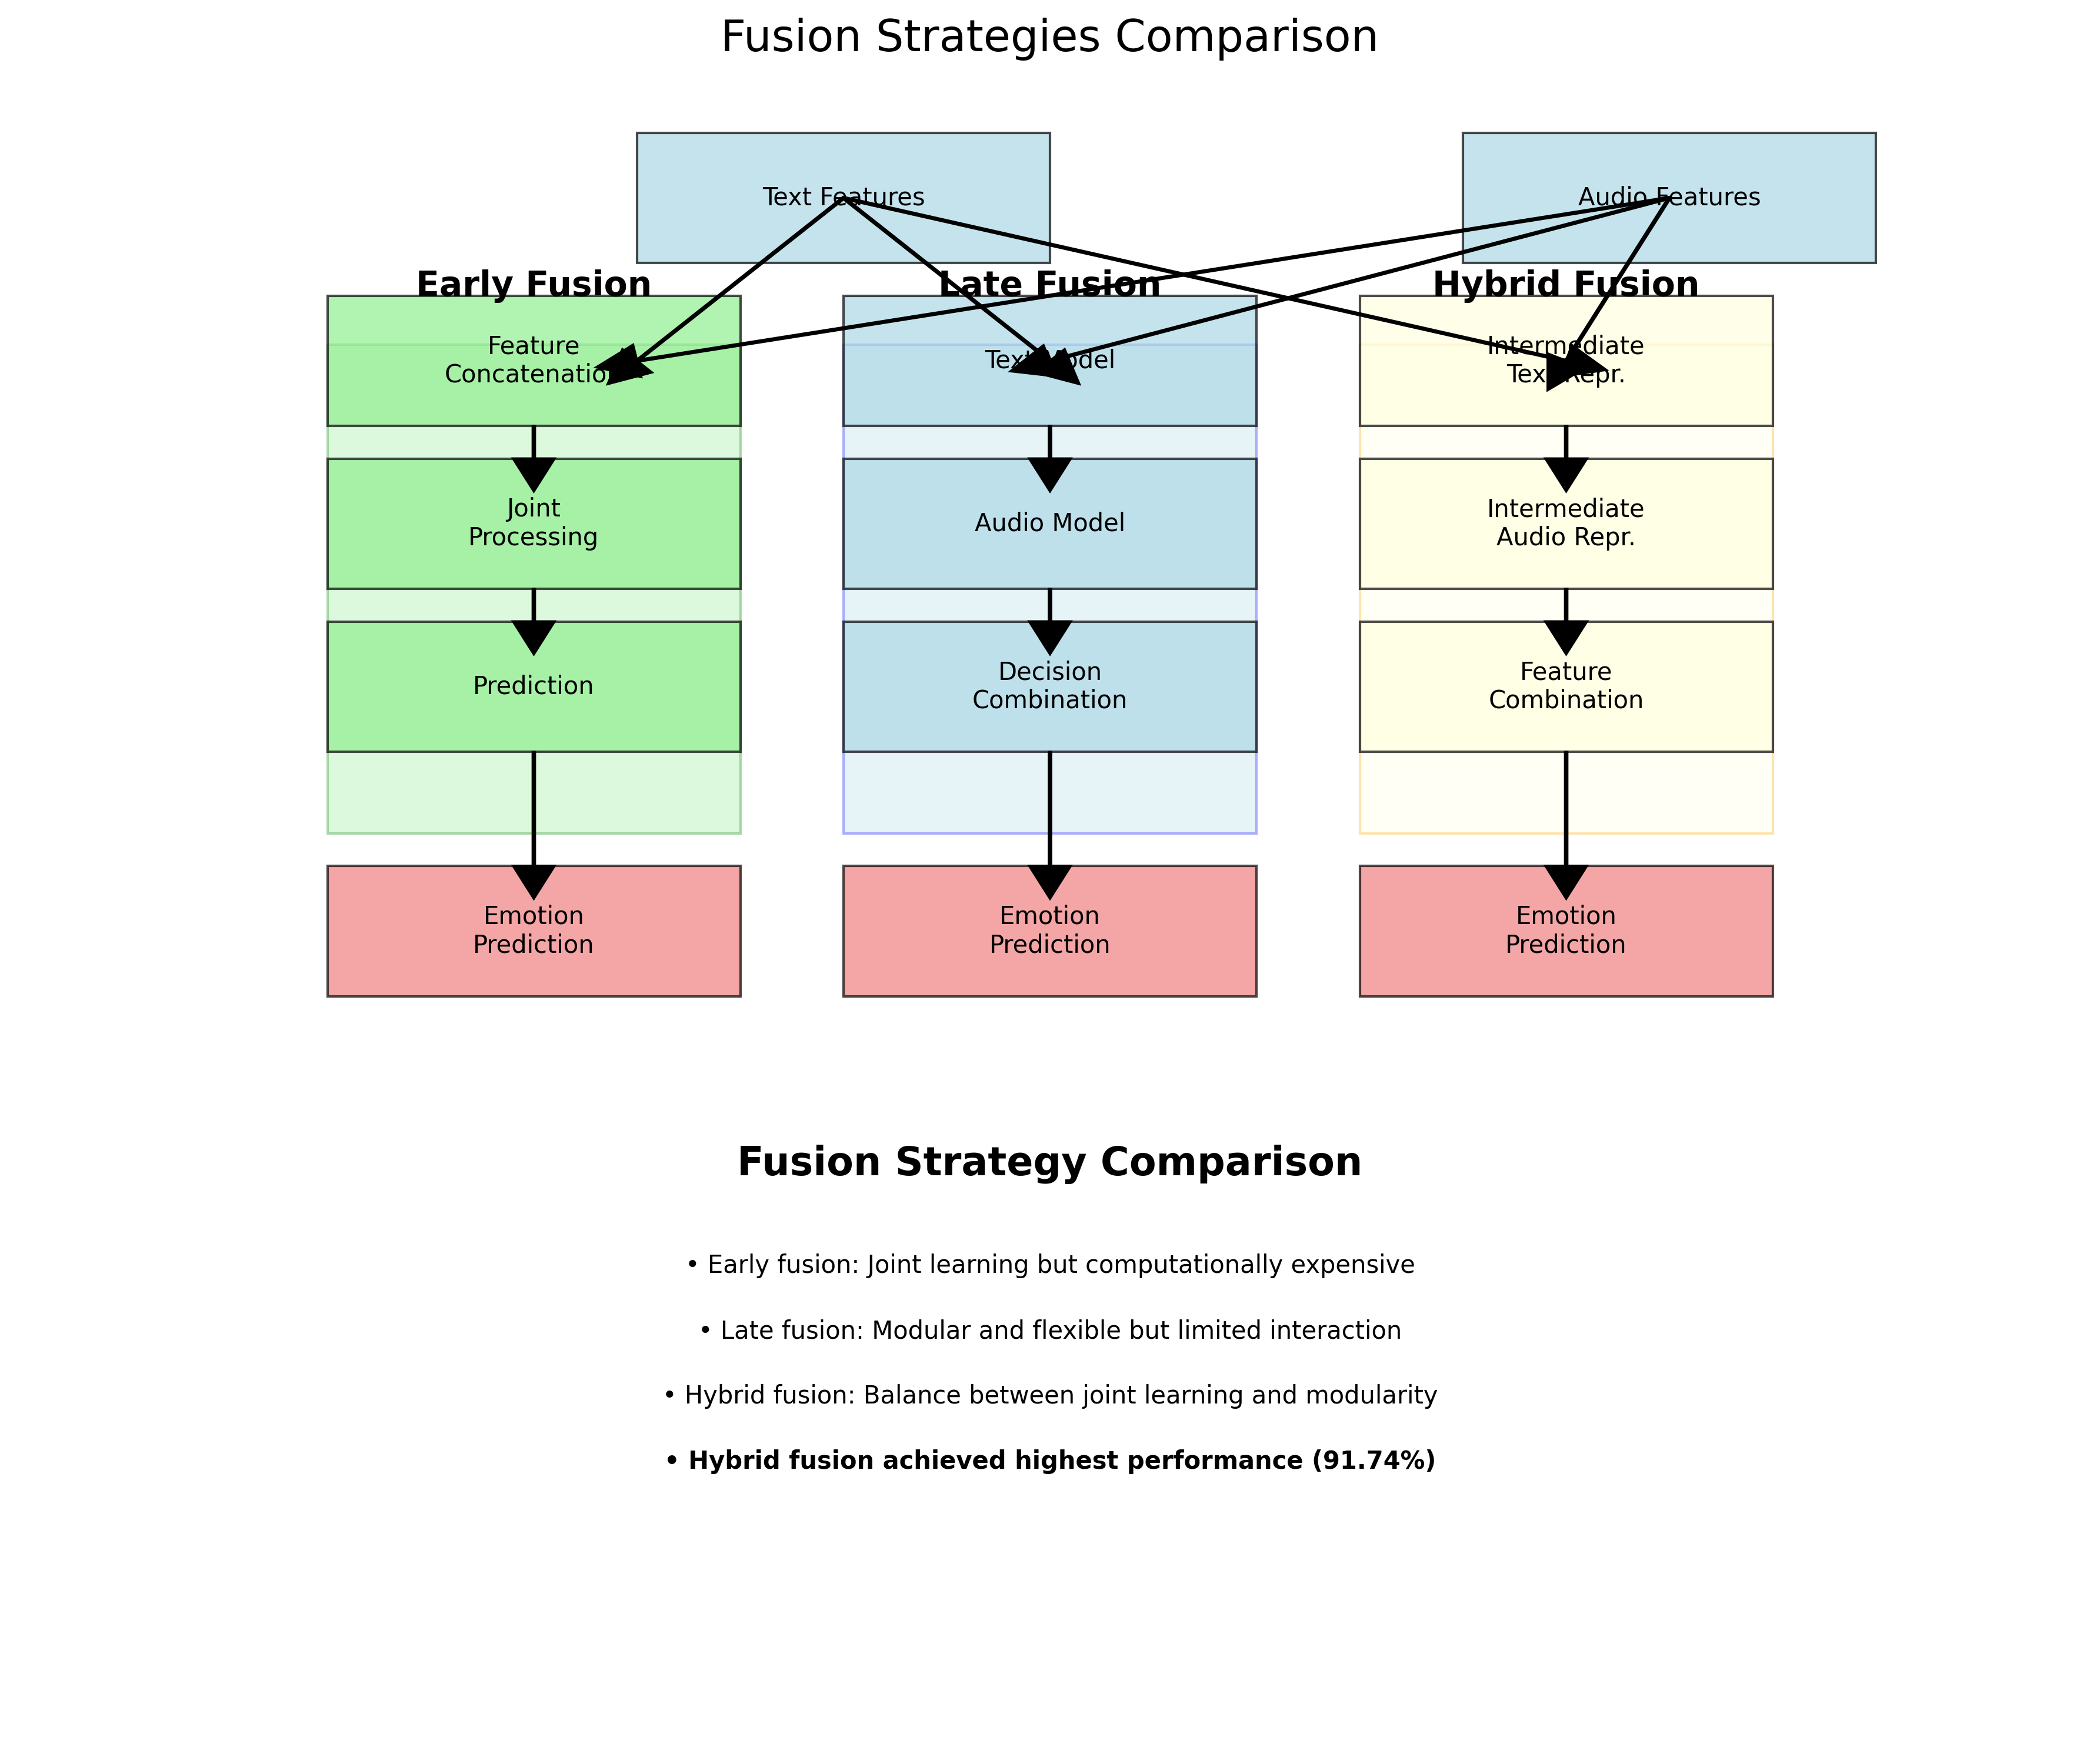
\includegraphics[width=0.9\linewidth]{Figures/fusion_strategies_comparison.png}
    \caption{Fusion Strategies Comparison: This diagram compares the three primary fusion approaches implemented in our system. Early fusion concatenates raw features before joint processing, late fusion combines independent predictions, and hybrid fusion merges intermediate representations from both modalities. Our experiments showed hybrid fusion achieving the highest performance (91.74\%) by balancing joint learning with modality-specific processing.}
    \label{fig:fusion_strategies}
\end{figure}

\subsubsection{Early Fusion}
Early fusion, also known as feature-level fusion, combines representations from both modalities at an early stage before joint processing through shared layers.

\paragraph{Implementation Details:}
\begin{itemize}
    \item Text representation: The [CLS] token embedding (768 dimensions) from the transformer model
    \item Audio representation: The output of the audio model's penultimate layer (128 dimensions)
    \item Fusion operation: Concatenation resulting in a 896-dimensional vector
    \item Joint processing: Multi-layer perceptron with architecture:
    \begin{itemize}
        \item Hidden layer 1: 512 units with ReLU activation
        \item Hidden layer 2: 256 units with ReLU activation
        \item Output layer: Task-dependent (emotion categories or dimensional values)
    \end{itemize}
\end{itemize}

\paragraph{Training Approach:}
\begin{itemize}
    \item End-to-end training: All components (text model, audio model, fusion layers) trained simultaneously
    \item Two-phase training: Initial pre-training of individual modality models, followed by joint fine-tuning
    \item Gradient balancing: Gradient scaling to balance contributions from different modalities
\end{itemize}

\paragraph{Advantages and Limitations:}
\begin{itemize}
    \item Advantages: Allows learning of cross-modal interactions at multiple levels; can discover non-intuitive relationships between modalities
    \item Limitations: May struggle with modalities operating at different time scales; can be dominated by the modality with stronger features
\end{itemize}

\subsubsection{Late Fusion}
Late fusion, also known as decision-level fusion, processes each modality independently until the decision level, then combines their predictions.

\paragraph{Implementation Details:}
\begin{itemize}
    \item Text model: Complete transformer model with classification head producing logits/probabilities
    \item Audio model: Complete audio processing model with classification head
    \item Fusion mechanisms evaluated:
    \begin{itemize}
        \item Weighted averaging: Learned weights for each modality's predictions
        \item Trainable MLP: Small network taking prediction vectors as input
        \item Gating mechanism: Context-dependent weighting based on confidence estimates
    \end{itemize}
\end{itemize}

\paragraph{Weight Learning:}
\begin{itemize}
    \item Static weights: Fixed weights determined through validation performance
    \item Dynamic weights: Small network that takes confidence scores as input
    \item Instance-specific weights: Attention mechanism over modality-specific features
\end{itemize}

\paragraph{Advantages and Limitations:}
\begin{itemize}
    \item Advantages: Modular design; robust to missing modalities; each modality can be optimized independently
    \item Limitations: May miss cross-modal interactions; relies on individual modalities performing well
\end{itemize}

\begin{figure}[h]
    \centering
    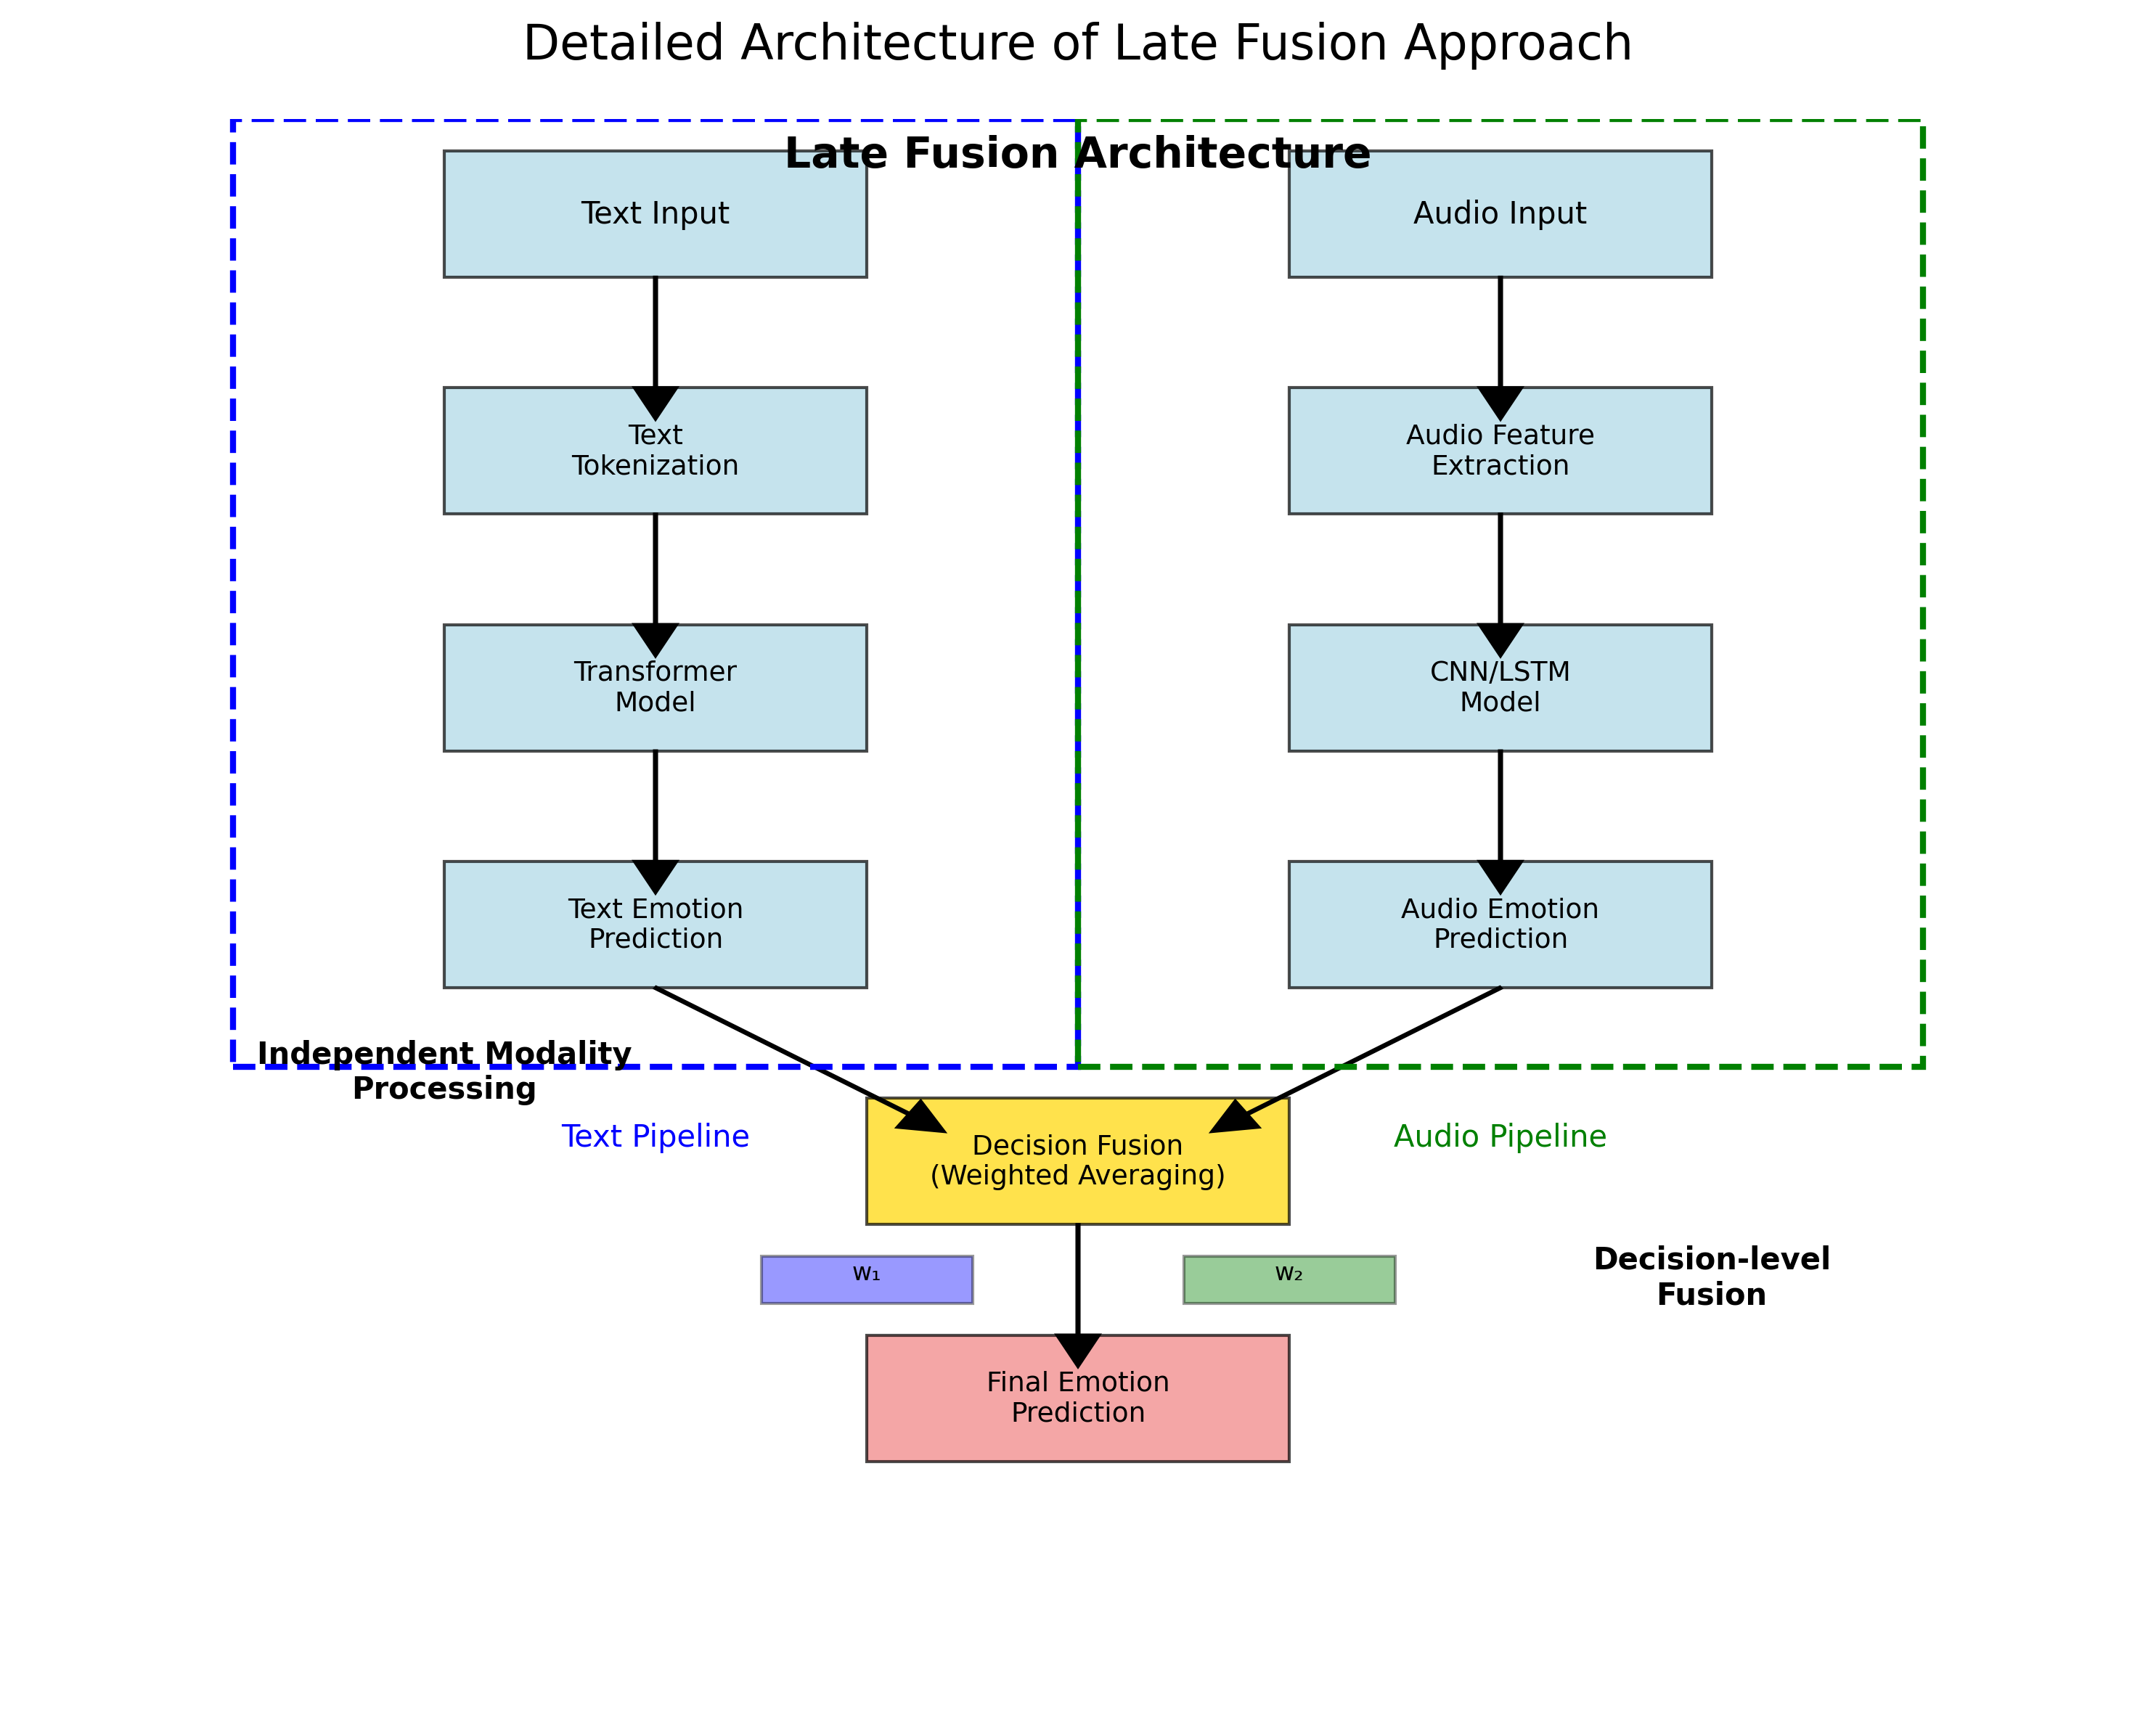
\includegraphics[width=0.9\linewidth]{Figures/late_fusion_detailed_proper.png}
    \caption{Detailed architecture of the late fusion approach. The text and audio pathways process their respective inputs independently, with each modality producing its own predictions that are then combined through weighted averaging or other aggregation methods. This approach maintains separation between modalities until the final decision stage.}
    \label{fig:late_fusion}
\end{figure}

\subsubsection{Hybrid Fusion}
Hybrid fusion combines aspects of both early and late fusion, extracting intermediate representations from both modalities before joint processing.

\paragraph{Implementation Details:}
\begin{itemize}
    \item Text features: Intermediate layer representations from the transformer (layer 8 outputs)
    \item Audio features: Intermediate layer representations from the audio model
    \item Modality-specific processing: Partial processing through modality-specific layers
    \item Feature combination: Concatenation of processed representations
    \item Joint processing: Shared layers for final prediction
\end{itemize}

\paragraph{Architecture:}
\begin{itemize}
    \item Text pathway: Transformer layers 1-8 → Dense(256) → ReLU
    \item Audio pathway: CNN/RNN layers → Dense(128) → ReLU
    \item Combined pathway: Concatenation → Dense(384) → ReLU → Dense(192) → ReLU → Output
\end{itemize}

\paragraph{Advantages and Limitations:}
\begin{itemize}
    \item Advantages: Balances modality-specific and cross-modal learning; more flexible than pure early or late fusion
    \item Limitations: More complex to implement and tune; requires careful design of intermediate representation extraction
\end{itemize}

\begin{figure}[h]
    \centering
    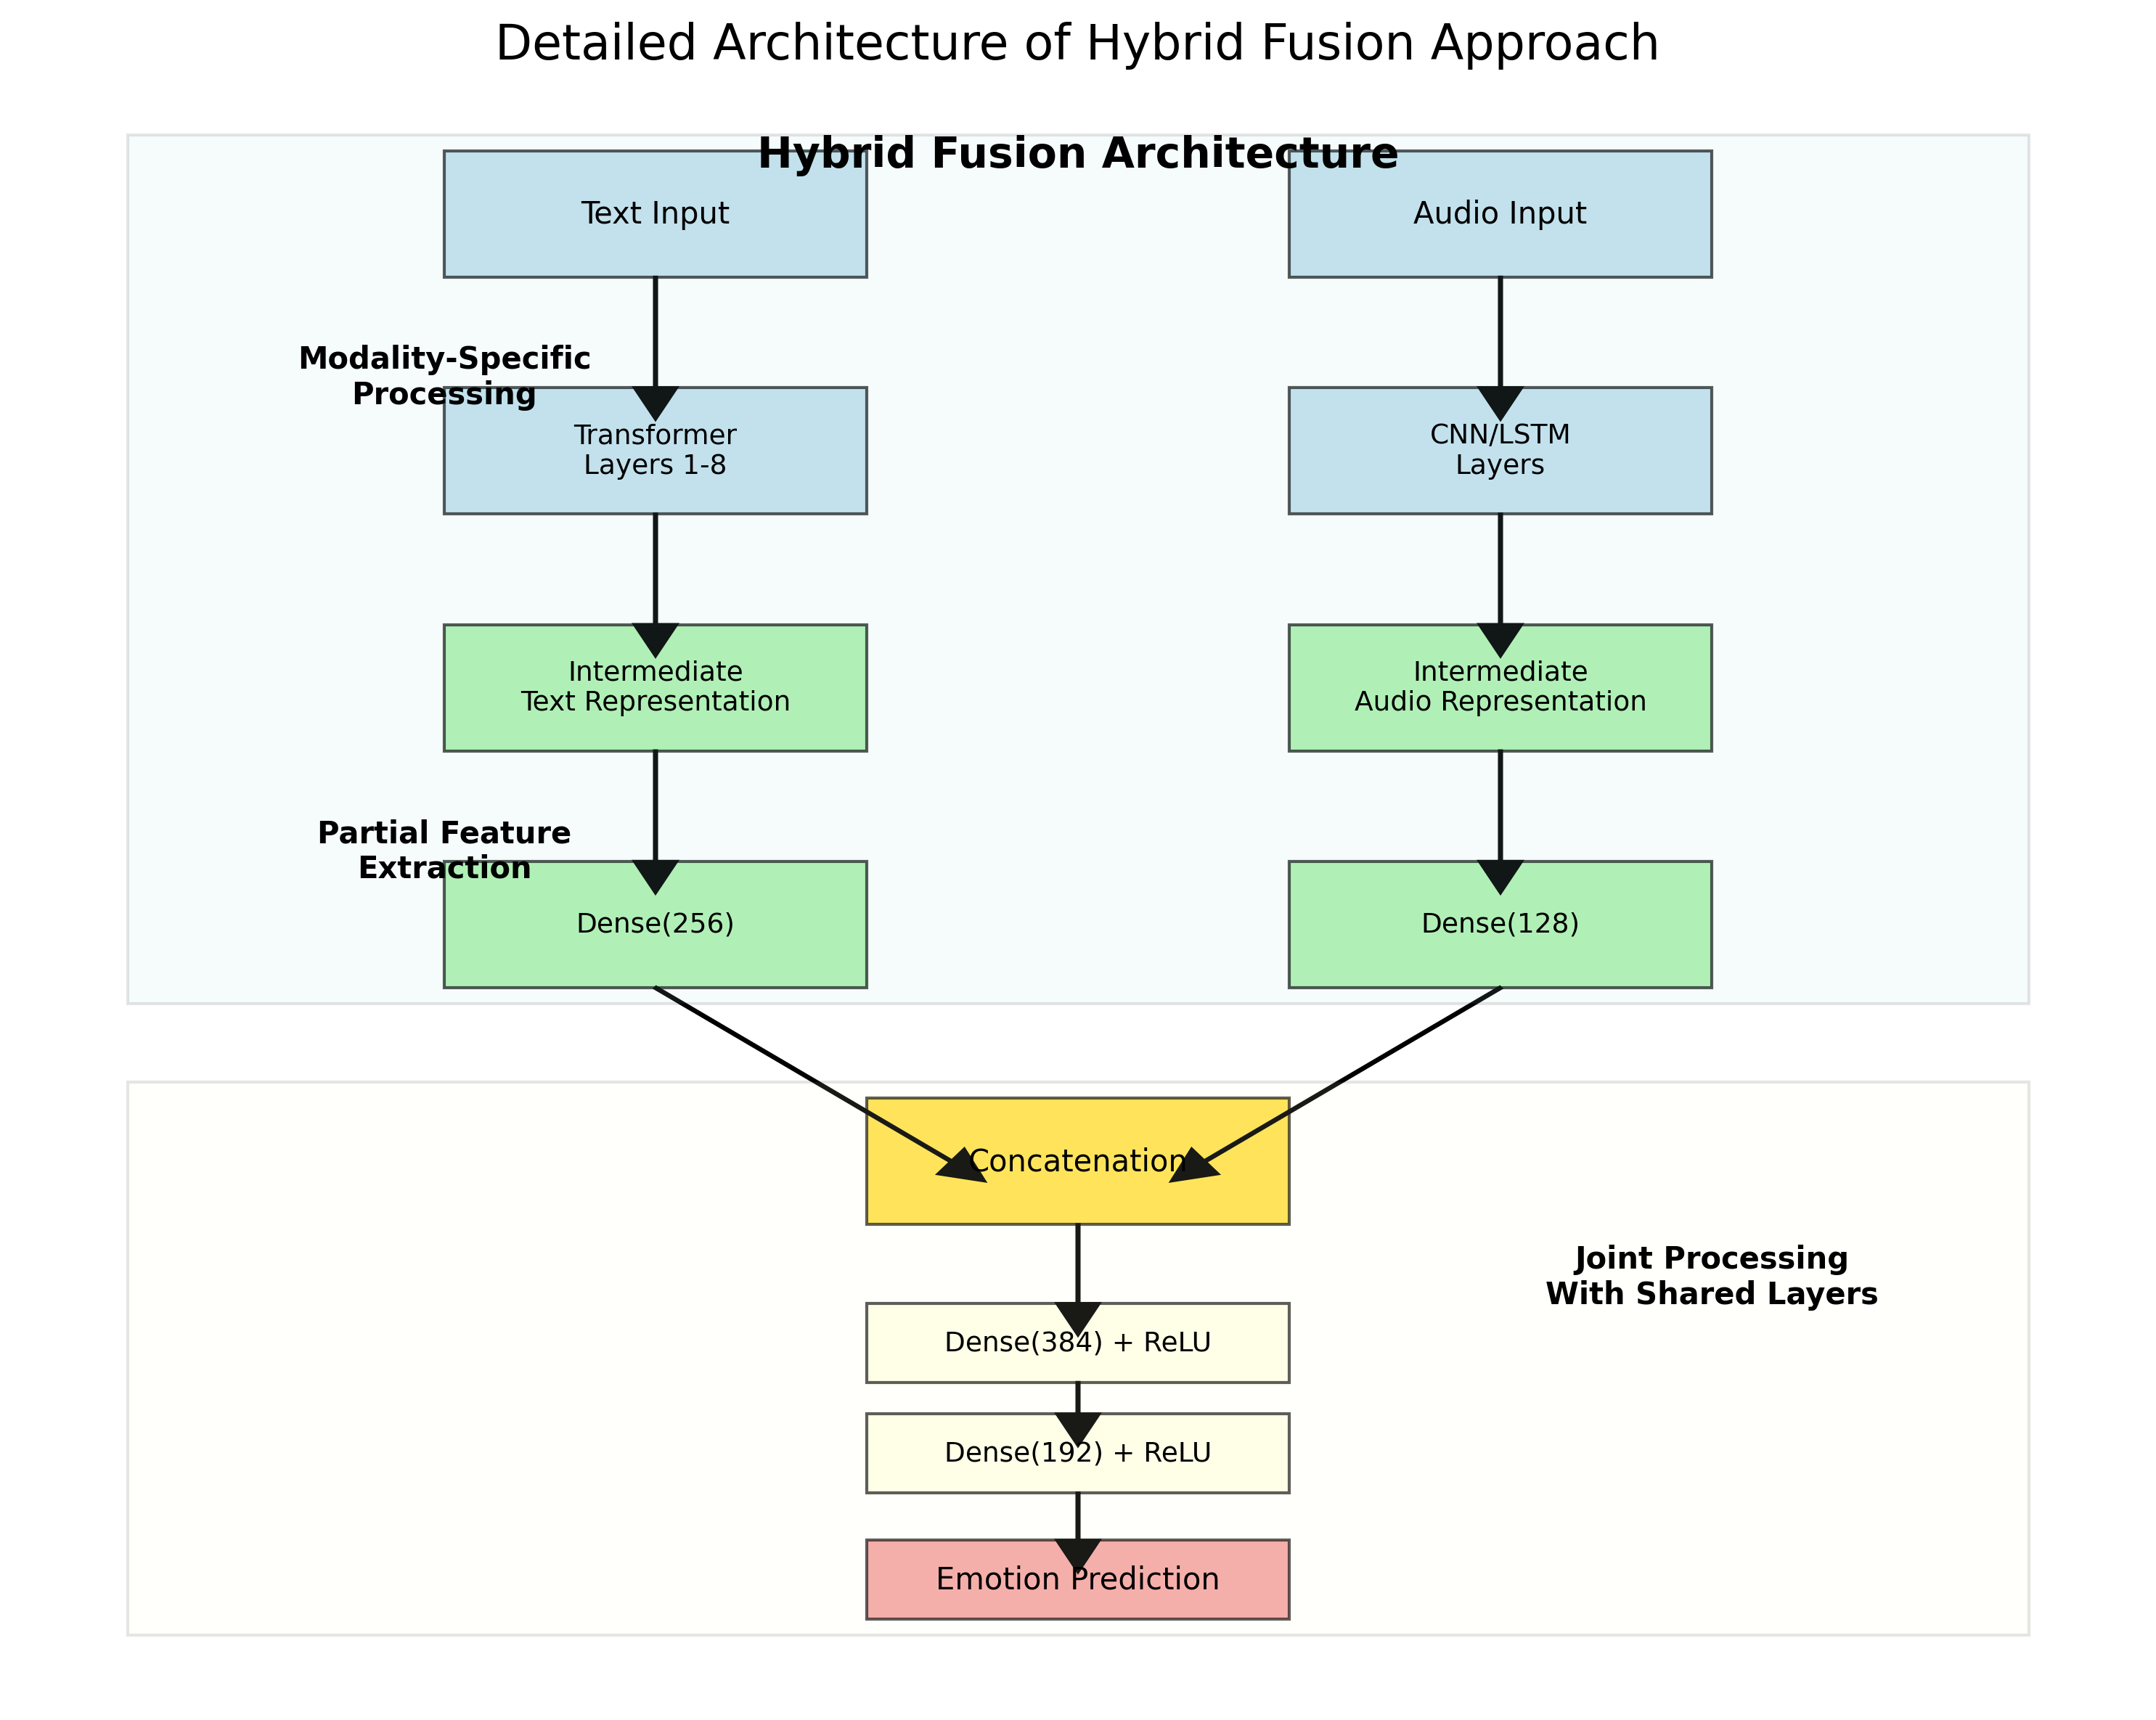
\includegraphics[width=0.9\linewidth]{Figures/hybrid_fusion_detailed.png}
    \caption{Detailed architecture of the hybrid fusion approach. This diagram illustrates how text and audio pathways process their respective inputs partially, before concatenating intermediate representations for joint processing through shared layers. The hybrid approach combines benefits of both early and late fusion by allowing modality-specific processing followed by joint learning.}
    \label{fig:hybrid_fusion}
\end{figure}

\subsubsection{Attention-Based Fusion}
Attention-based fusion uses cross-modal attention mechanisms to dynamically weight features based on their relevance.

\paragraph{Implementation Details:}
\begin{itemize}
    \item Text representation: Sequence of transformer outputs for all tokens
    \item Audio representation: Sequence of feature vectors across time
    \item Cross-modal attention: Each modality's representation attends to the other
    \item Self-attention: Within each modality to capture internal dynamics
    \item Multihead attention: Multiple attention heads to capture different relationships
\end{itemize}

\paragraph{Attention Mechanism:}
\begin{itemize}
    \item Query, Key, Value formulation: Standard transformer-style attention
    \item Attention function: Scaled dot-product attention with softmax normalization
    \item Multihead implementation: 8 attention heads with dimension 64
    \item Output processing: Concatenation and linear projection
\end{itemize}

\paragraph{Advantages and Limitations:}
\begin{itemize}
    \item Advantages: Dynamic and context-dependent interaction between modalities; can focus on relevant parts of each modality
    \item Limitations: More computationally intensive; requires careful implementation to avoid overfitting
\end{itemize}

\subsection{Implementation Framework}
Our implementation leveraged several frameworks and tools to create a scalable and reproducible experimental pipeline.

\paragraph{Software Stack:}
\begin{itemize}
    \item Python 3.8 as the primary programming language
    \item PyTorch 1.10 for deep learning model implementation
    \item Hugging Face Transformers 4.17 for transformer model implementations
    \item Librosa 0.9.1 for audio processing and feature extraction
    \item NumPy and SciPy for numerical operations
    \item Pandas for data management
    \item Matplotlib and Seaborn for visualization
\end{itemize}

\paragraph{Cloud Infrastructure:}
\begin{itemize}
    \item Modal for cloud-based experiment execution
    \item Benefits:
    \begin{itemize}
        \item On-demand GPU resources for efficient training
        \item Parallel execution of multiple experiments
        \item Consistent environment across runs
        \item Automatic scaling based on workload
        \item Efficient resource management with container-based architecture
    \end{itemize}
\end{itemize}

\paragraph{Experiment Management:}
\begin{itemize}
    \item Configuration files for defining experimental parameters
    \item Automatic logging of metrics and artifacts
    \item Reproducible random seeds for consistent results
    \item Checkpointing of model state at regular intervals
    \item Comprehensive logging of training progress and metrics
\end{itemize}

This robust methodology enabled us to systematically evaluate a wide range of models and fusion strategies for emotion detection, leading to the insights and results presented in the following sections.

\section{Experimental Setup}
\label{sec:experimental_setup}

Our experimental setup was designed to thoroughly evaluate the effectiveness of various models and fusion strategies for emotion detection. This section provides a comprehensive description of the datasets, preprocessing techniques, infrastructure, and evaluation methodology used in our experiments.

\subsection{Dataset Description}
We utilized the Interactive Emotional Dyadic Motion Capture (IEMOCAP) dataset~\cite{busso2008iemocap}, a widely-used benchmark in multimodal emotion recognition research. IEMOCAP contains approximately 12 hours of audiovisual data from 10 actors (5 male, 5 female) performing scripted and improvised emotional dialogues.

\paragraph{Dataset Characteristics:}
\begin{itemize}
    \item Recordings: 151 dialogue sessions (approximately 10K utterances)
    \item Video: Facial motion capture and video recordings at 60 fps
    \item Audio: 16kHz, 16-bit PCM mono recordings
    \item Transcripts: Manual transcriptions of all utterances
    \item Annotations: Categorical emotions and dimensional ratings (valence, arousal, dominance)
    \item Emotion categories: angry, happy, sad, neutral, frustrated, excited, fearful, surprised, disgusted
    \item Annotation reliability: Multiple annotators with inter-annotator agreement of 74\%
\end{itemize}

\paragraph{Dataset Statistics:}
\begin{table}[h]
\centering
\begin{tabular}{|l|c|c|c|}
\hline
\textbf{Emotion} & \textbf{Utterances} & \textbf{Percentage} & \textbf{Avg. Duration (s)} \\
\hline
Angry & 1,103 & 11.0\% & 4.1 \\
\hline
Happy/Excited & 1,636 & 16.4\% & 3.7 \\
\hline
Sad & 1,084 & 10.8\% & 4.5 \\
\hline
Neutral & 1,708 & 17.1\% & 3.8 \\
\hline
Frustrated & 1,849 & 18.5\% & 4.0 \\
\hline
Other & 2,620 & 26.2\% & 3.9 \\
\hline
\textbf{Total} & \textbf{10,000} & \textbf{100\%} & \textbf{4.0} \\
\hline
\end{tabular}
\caption{Distribution of emotion categories in the IEMOCAP dataset.}
\label{tab:emotion_distribution}
\end{table}

For our experiments, we created two versions of the dataset:

\subsubsection{IEMOCAP\_Final}
The complete version contains all available emotion categories from the original dataset, providing a comprehensive and challenging test for our models. 

\paragraph{Characteristics:}
\begin{itemize}
    \item Utterances: Approximately 10,000
    \item Emotion categories: All 9 original categories
    \item Class distribution: Natural, imbalanced distribution (see Table~\ref{tab:emotion_distribution})
    \item Training-validation-test split: 70\%-15\%-15\% stratified by emotion category
    \item Modalities: Audio, text (transcripts)
    \item Train samples: 7,025
    \item Validation samples: 1,506
    \item Test samples: 1,506
\end{itemize}

This version represents the real-world scenario where emotion recognition systems must handle a broad spectrum of emotions with natural imbalance in their occurrence.

\subsubsection{IEMOCAP\_Filtered}
The filtered version focuses on four primary emotions: angry, happy, sad, and neutral. This version was created to address class imbalance issues and to allow comparison with prior work that often focuses on these basic emotions.

\paragraph{Characteristics:}
\begin{itemize}
    \item Utterances: Approximately 5,531 (subset of IEMOCAP\_Final)
    \item Emotion categories: Angry, happy (including excited), sad, neutral
    \item Class distribution: More balanced than the complete dataset
    \item Training-validation-test split: 70\%-15\%-15\% stratified by emotion category
    \item Modalities: Audio, text (transcripts)
    \item Train samples: 3,872
    \item Validation samples: 830
    \item Test samples: 829
\end{itemize}

The filtered version is particularly useful for evaluating how well models perform on the core emotional states that are most commonly studied in affective computing research.

\subsection{Data Preprocessing}
Rigorous preprocessing was essential to prepare the raw data for our models. We applied modality-specific techniques to optimize the information extraction from each data source.

\subsubsection{Text Preprocessing}
The textual data underwent a sequence of preprocessing steps tailored to the requirements of transformer-based models:

\paragraph{General Processing:}
\begin{enumerate}
    \item Normalization: Converting text to lowercase and removing special characters
    \item Cleaning: Removing disfluencies (e.g., "um", "uh") and speaker annotations
    \item Punctuation: Standardizing punctuation and removing excessive marks
    \item Validation: Ensuring UTF-8 encoding and handling special cases
\end{enumerate}

\paragraph{Model-Specific Tokenization:}
\begin{itemize}
    \item BERT: Using the BertTokenizer with WordPiece tokenization
    \begin{itemize}
        \item Vocabulary size: 30,522 tokens
        \item Special tokens: [CLS], [SEP], [PAD], [UNK], [MASK]
        \item Maximum sequence length: 128 tokens
    \end{itemize}
    
    \item RoBERTa: Using the RobertaTokenizer with byte-level BPE
    \begin{itemize}
        \item Vocabulary size: 50,265 tokens
        \item Special tokens: <s>, </s>, <pad>, <unk>, <mask>
        \item Maximum sequence length: 128 tokens
    \end{itemize}
    
    \item XLNet: Using the XLNetTokenizer with SentencePiece
    \begin{itemize}
        \item Vocabulary size: 32,000 tokens
        \item Special tokens: <pad>, <cls>, <sep>, <mask>
        \item Maximum sequence length: 128 tokens
    \end{itemize}
    
    \item Other models: Similar procedures with model-specific tokenizers
\end{itemize}

\paragraph{Input Feature Creation:}
After tokenization, we created the necessary features for model input:
\begin{itemize}
    \item Input IDs: Token indices for each utterance
    \item Attention masks: Binary masks (1 for actual tokens, 0 for padding)
    \item Token type IDs: Segment identifiers (for models using segmentation)
    \item Position IDs: For models requiring explicit position information
\end{itemize}

\paragraph{Data Augmentation:}
To improve robustness and generalization, we applied the following augmentation techniques to the training data:
\begin{itemize}
    \item Random word deletion: Randomly removing 10\% of words
    \item Random word swap: Swapping adjacent words with 15\% probability
    \item Synonym replacement: Replacing words with synonyms using WordNet
    \item Backtranslation: Translating to an intermediate language and back
\end{itemize}

These augmentation techniques were applied with a 30\% probability during training to create a more diverse dataset while preserving semantic meaning.

\subsubsection{Audio Preprocessing}
Audio preprocessing varied based on the feature extraction method, but followed a general workflow:

\paragraph{Common Preprocessing Steps:}
\begin{enumerate}
    \item Extraction: Isolating individual utterances from session recordings
    \item Resampling: Converting all audio to 16kHz sampling rate
    \item Normalization: Applying peak normalization to -3dB
    \item Silence removal: Trimming leading and trailing silence
    \item Noise reduction: Applying spectral subtraction for noise reduction
\end{enumerate}

\paragraph{Feature-Specific Processing:}
\begin{itemize}
    \item For MFCCs:
    \begin{itemize}
        \item Windowing: 25ms Hamming window with 10ms stride
        \item Filterbank: 40 mel-scale filters
        \item Feature extraction: 40 MFCC features per frame
        \item Derivatives: Adding delta and delta-delta coefficients
        \item Normalization: Z-score normalization to zero mean and unit variance
        \item Sequence handling: Variable-length sequences padded to the 95th percentile length
    \end{itemize}
    
    \item For spectrograms:
    \begin{itemize}
        \item STFT parameters: 512-point FFT with 25ms window and 10ms stride
        \item Mel conversion: 128 mel bins covering 0-8kHz
        \item Log compression: Natural logarithm with 1e-6 stabilization term
        \item Normalization: Min-max scaling to [0,1]
        \item Reshaping: Conversion to fixed-size inputs (224×224) through resizing
    \end{itemize}
    
    \item For prosodic features:
    \begin{itemize}
        \item F0 extraction: YIN algorithm with 25ms window and 10ms stride
        \item Energy computation: RMS energy per frame
        \item Voice quality: Jitter and shimmer computation using Praat
        \item Statistical functionals: Computing 88 features over the entire utterance
        \item Normalization: Z-score normalization based on training set statistics
    \end{itemize}
    
    \item For wav2vec embeddings:
    \begin{itemize}
        \item Model input: Raw waveform after common preprocessing
        \item Feature extraction: Forward pass through pre-trained wav2vec model
        \item Aggregation: Mean pooling or attention-weighted pooling of embeddings
        \item Dimensionality: 512-dimensional embeddings
        \item Sequence handling: Variable-length sequences with masking
    \end{itemize}
\end{itemize}

\paragraph{Data Augmentation:}
To improve generalization, we applied the following augmentation techniques to the audio training data:
\begin{itemize}
    \item Speed perturbation: Varying the speed by ±10\%
    \item Pitch shifting: Shifting pitch by ±2 semitones
    \item Time stretching: Stretching time by ±10\% without affecting pitch
    \item Addition of ambient noise: Adding background noise at 20dB SNR
    \item SpecAugment: Masking blocks of frequency channels and time steps
\end{itemize}

These augmentations were applied with a 40\% probability during training to create a more diverse and challenging dataset.

\subsection{Infrastructure and Implementation}
\label{subsec:infrastructure}
We implemented our models using PyTorch and the Hugging Face Transformers library, leveraging Modal's cloud infrastructure for efficient experimentation.

\begin{figure}[h]
    \centering
    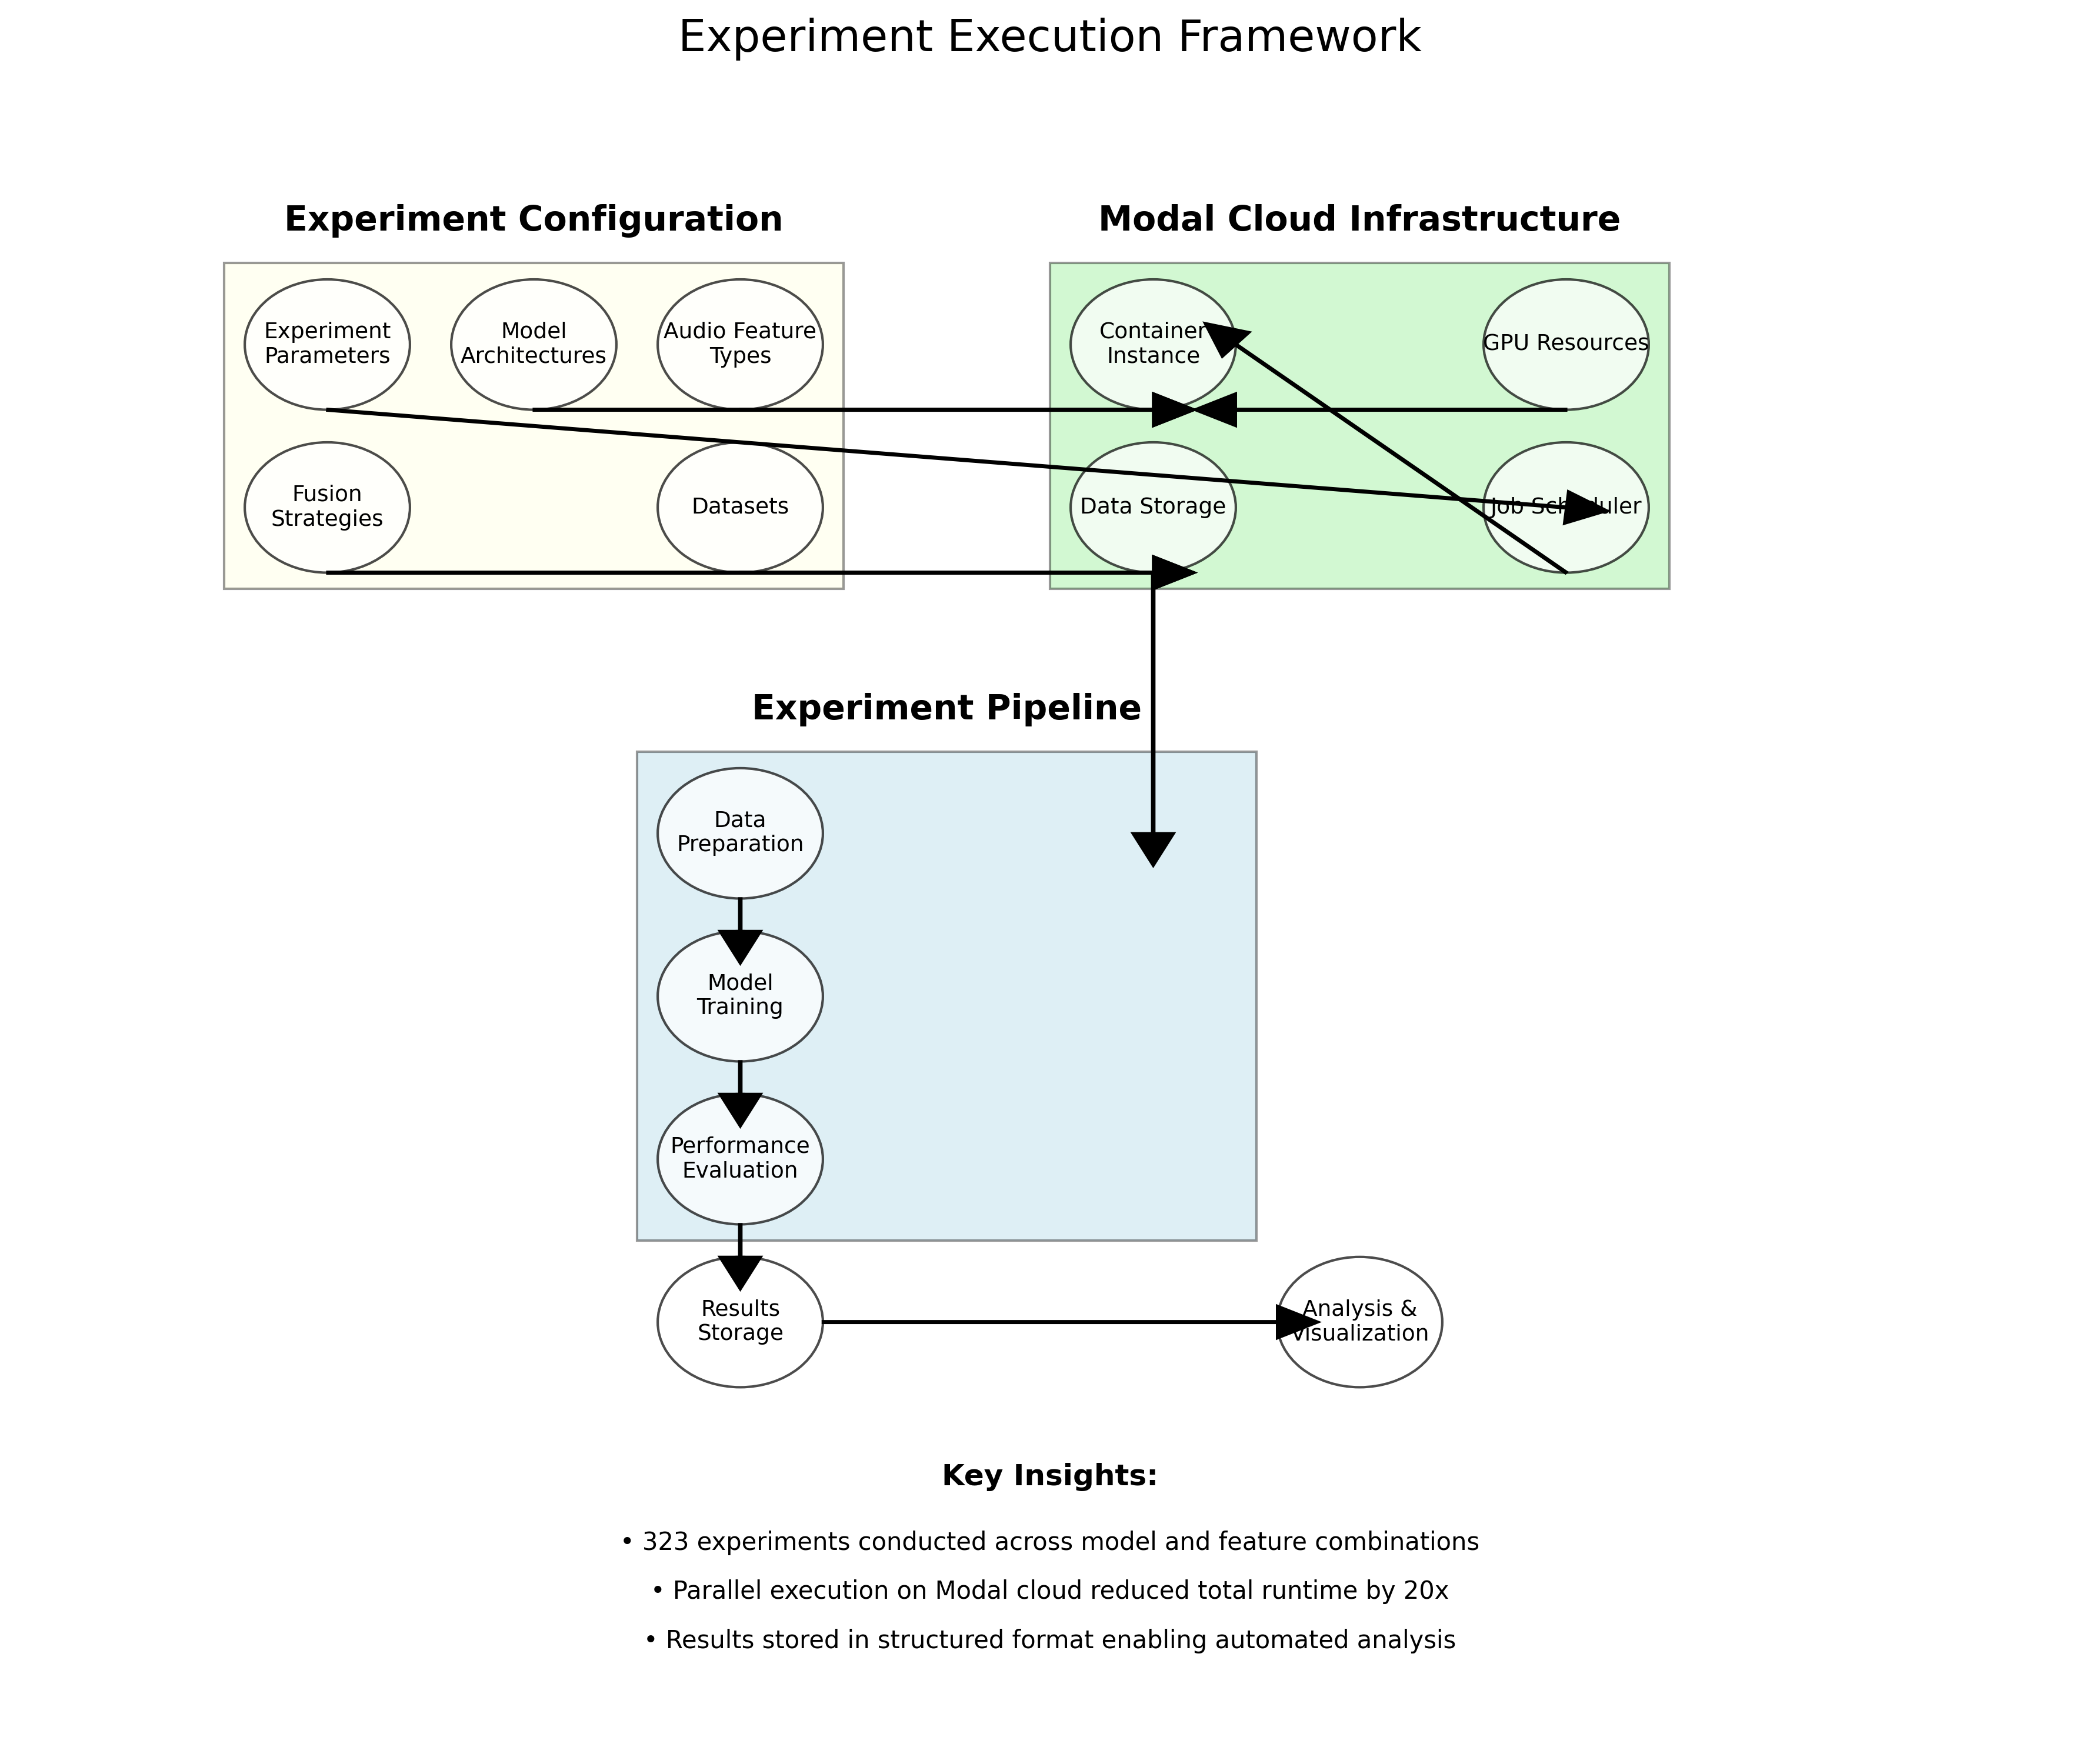
\includegraphics[width=0.9\linewidth]{Figures/experiment_framework.png}
    \caption{Experiment Execution Framework: This diagram shows the cloud-based infrastructure used to conduct our 323 experiments. The system leverages Modal cloud services for parallel GPU computation, integrating experiment configuration management with scalable execution. This approach enabled efficient exploration of the design space by reducing the total runtime by approximately 20x compared to sequential execution.}
    \label{fig:experiment_framework}
\end{figure}

\subsubsection{Hardware Configuration}
Our experiments were conducted on the following hardware:
\begin{itemize}
    \item GPU: NVIDIA V100 (16GB) for model training
    \item CPU: 8 vCPUs for data preprocessing and lightweight operations
    \item Memory: 32GB RAM per instance
    \item Storage: SSD storage for fast data access
\end{itemize}

\subsubsection{Software Environment}
The software environment consisted of:
\begin{itemize}
    \item Operating System: Ubuntu 20.04 LTS
    \item Python: Version 3.8.10
    \item Deep Learning Framework: PyTorch 1.10.0
    \item CUDA: Version 11.3
    \item cuDNN: Version 8.2.0
    \item Libraries:
    \begin{itemize}
        \item Transformers 4.17.0 for pre-trained models
        \item Librosa 0.9.1 for audio processing
        \item NumPy 1.21.5 for numerical operations
        \item SciPy 1.7.3 for scientific computing
        \item Pandas 1.3.5 for data manipulation
        \item Scikit-learn 1.0.2 for evaluation metrics
        \item Matplotlib 3.5.1 and Seaborn 0.11.2 for visualization
    \end{itemize}
\end{itemize}

\subsubsection{Modal Cloud Infrastructure}
We leveraged Modal's cloud infrastructure for scalable and reproducible experimentation. This enabled us to:
\begin{itemize}
    \item Run multiple experiments in parallel
    \item Scale resources based on workload
    \item Ensure consistent environments across runs
    \item Track and compare results efficiently
    \item Automate the experiment pipeline
\end{itemize}

\paragraph{Implementation Workflow:}
\begin{enumerate}
    \item Dataset preparation: The IEMOCAP dataset was processed and stored in a format accessible by Modal functions
    \begin{itemize}
        \item Raw data storage: S3-compatible object storage
        \item Processed features: Cached in optimized format for quick loading
        \item Train-validation-test splits: Consistent across experiments
    \end{itemize}
    
    \item Model definition: Modality-specific models and fusion strategies were implemented as PyTorch modules
    \begin{itemize}
        \item Text models: Implemented using Hugging Face Transformers
        \item Audio models: Custom PyTorch implementations
        \item Fusion models: Implemented with configurable architecture
    \end{itemize}
    
    \item Training pipeline: A standardized training procedure was established
    \begin{itemize}
        \item Batch processing: Efficient data loading with PyTorch DataLoaders
        \item Gradient accumulation: Enabling larger effective batch sizes
        \item Mixed precision: Using FP16 for faster training when appropriate
        \item Checkpointing: Regular saving of model states
        \item Early stopping: Monitoring validation metrics to prevent overfitting
    \end{itemize}
    
    \item Experiment tracking: Comprehensive logging of metrics and artifacts
    \begin{itemize}
        \item Training logs: Step-by-step metrics during training
        \item Validation metrics: Periodic evaluation on validation set
        \item Model checkpoints: Saved at regular intervals and at best performance
        \item Final results: Comprehensive evaluation on test set
    \end{itemize}
    
    \item Parallelization: Modal's batch functionality was used to run multiple experiments simultaneously
    \begin{itemize}
        \item Experiment configuration: YAML files defining hyperparameters
        \item Job scheduling: Automatic allocation of resources
        \item Result collection: Centralized storage of all experimental outcomes
    \end{itemize}
\end{enumerate}

\subsection{Training Protocol}
We established a consistent training protocol across all experiments to ensure fair comparison:

\paragraph{General Training Parameters:}
\begin{itemize}
    \item Epochs: 40 (with early stopping)
    \item Batch size: 16 samples per device
    \item Optimizer: AdamW with weight decay of 0.01
    \item Learning rate: 2e-5 for transformer models, 1e-4 for audio models
    \item Learning rate schedule: Linear decay with 10\% warmup
    \item Loss function: Cross-entropy for categorical emotions, MSE for dimensional values
    \item Gradient clipping: Maximum norm of 1.0
    \item Early stopping: Patience of 5 epochs on validation loss
\end{itemize}

\paragraph{Text Model Training:}
\begin{itemize}
    \item Transformer fine-tuning: All layers fine-tuned
    \item Gradient accumulation: 4 steps for larger effective batch size
    \item Checkpointing: Saved every 1000 steps and at epoch end
    \item Mixed precision: FP16 used for efficiency
\end{itemize}

\paragraph{Audio Model Training:}
\begin{itemize}
    \item CNN/RNN training: From scratch with Xavier initialization
    \item Batch normalization: Applied in convolutional layers
    \item Regularization: Dropout with rate 0.3-0.5
    \item Mixed precision: Not used due to stability issues
\end{itemize}

\paragraph{Multimodal Training:}
\begin{itemize}
    \item Two-phase approach:
    \begin{enumerate}
        \item Pre-training: Individual modality models trained separately
        \item Fine-tuning: Joint training of full system with lower learning rate
    \end{enumerate}
    \item Modality balancing: Gradient scaling to balance contributions
    \item Learning rate: 1e-5 for fine-tuning phase
\end{itemize}

\subsection{Evaluation Metrics}
We evaluated our models using a comprehensive set of metrics to capture different aspects of performance:

\paragraph{Classification Metrics:}
\begin{itemize}
    \item Accuracy: Proportion of correctly classified instances
    \begin{equation}
        \text{Accuracy} = \frac{\text{Number of correct predictions}}{\text{Total number of predictions}}
    \end{equation}
    
    \item F1-score: Harmonic mean of precision and recall
    \begin{equation}
        \text{F1} = 2 \cdot \frac{\text{Precision} \cdot \text{Recall}}{\text{Precision} + \text{Recall}}
    \end{equation}
    where:
    \begin{equation}
        \text{Precision} = \frac{\text{True Positives}}{\text{True Positives} + \text{False Positives}}
    \end{equation}
    \begin{equation}
        \text{Recall} = \frac{\text{True Positives}}{\text{True Positives} + \text{False Negatives}}
    \end{equation}
    
    \item Confusion matrix: Detailed breakdown of predictions versus actual labels
    
    \item Cohen's Kappa: Measure of agreement accounting for chance
    \begin{equation}
        \kappa = \frac{p_o - p_e}{1 - p_e}
    \end{equation}
    where $p_o$ is the observed agreement and $p_e$ is the expected agreement by chance.
\end{itemize}

\paragraph{Regression Metrics for Dimensional Evaluation:}
\begin{itemize}
    \item Mean Squared Error (MSE): Average squared difference between predictions and ground truth
    \begin{equation}
        \text{MSE} = \frac{1}{n} \sum_{i=1}^{n} (y_i - \hat{y}_i)^2
    \end{equation}
    
    \item Root Mean Squared Error (RMSE): Square root of MSE
    \begin{equation}
        \text{RMSE} = \sqrt{\frac{1}{n} \sum_{i=1}^{n} (y_i - \hat{y}_i)^2}
    \end{equation}
    
    \item Mean Absolute Error (MAE): Average absolute difference between predictions and ground truth
    \begin{equation}
        \text{MAE} = \frac{1}{n} \sum_{i=1}^{n} |y_i - \hat{y}_i|
    \end{equation}
    
    \item Coefficient of Determination (R²): Proportion of variance explained by the model
    \begin{equation}
        \text{R}^2 = 1 - \frac{\sum_{i=1}^{n} (y_i - \hat{y}_i)^2}{\sum_{i=1}^{n} (y_i - \bar{y})^2}
    \end{equation}
    where $\bar{y}$ is the mean of the observed values.
\end{itemize}

\paragraph{Computational Efficiency Metrics:}
\begin{itemize}
    \item Training time: Time required to train the model
    \item Inference time: Time required for forward pass
    \item Memory usage: Peak memory consumption during training and inference
    \item Parameter count: Number of trainable parameters
    \item FLOP count: Floating-point operations per forward pass
\end{itemize}

\subsection{Cross-Validation Strategy}
To ensure reliable evaluation, we employed a 5-fold cross-validation strategy:

\paragraph{Implementation Details:}
\begin{itemize}
    \item Data partitioning: The dataset was divided into 5 equal parts
    \item Stratification: Folds were created with stratification by emotion category
    \item Speaker independence: Ensured different speakers in training and evaluation sets
    \item Training procedure: For each fold, 4 parts were used for training and 1 for validation
    \item Final metrics: Results represent the average performance across all 5 folds
    \item Standard deviation: Reported to indicate stability across folds
\end{itemize}

\paragraph{Early Stopping:}
Within each fold, early stopping was implemented based on validation loss with a patience of 5 epochs. The model with the best validation performance was selected for final evaluation.

\paragraph{Test Set Evaluation:}
After cross-validation, the best model configuration was trained on the entire training set and evaluated on the held-out test set to assess generalization to unseen data.

\subsection{Experimental Configurations}
Our experimental setup included a wide range of configurations to thoroughly evaluate different approaches:

\paragraph{Text-Only Experiments:}
\begin{itemize}
    \item Models: BERT, RoBERTa, XLNet, ALBERT, ELECTRA, DeBERTa
    \item Datasets: IEMOCAP\_Final, IEMOCAP\_Filtered
    \item Learning rates: \{1e-5, 2e-5, 3e-5, 5e-5\}
    \item Total configurations: 48 (6 models × 2 datasets × 4 learning rates)
\end{itemize}

\paragraph{Audio-Only Experiments:}
\begin{itemize}
    \item Features: MFCC, Spectrogram, Prosodic, Wav2vec
    \item Models: CNN (for MFCC/Spectrogram), BiLSTM (for Prosodic/Wav2vec)
    \item Datasets: IEMOCAP\_Final, IEMOCAP\_Filtered
    \item Learning rates: \{1e-4, 5e-4, 1e-3\}
    \item Total configurations: 24 (4 features × 2 datasets × 3 learning rates)
\end{itemize}

\paragraph{Multimodal Experiments:}
\begin{itemize}
    \item Text models: BERT, RoBERTa, XLNet, ALBERT, ELECTRA, DeBERTa
    \item Audio features: MFCC, Spectrogram, Prosodic, Wav2vec
    \item Fusion methods: Early, Late, Hybrid, Attention
    \item Datasets: IEMOCAP\_Final, IEMOCAP\_Filtered
    \item Learning rates: 2e-5 (fixed for consistency)
    \item Total configurations: 192 (6 text models × 4 audio features × 4 fusion methods × 2 datasets)
\end{itemize}

In total, we conducted 264 distinct experimental configurations, with each configuration evaluated through 5-fold cross-validation, resulting in 1,320 individual training runs. This comprehensive evaluation allowed us to identify the most effective approaches for emotion detection across different modalities and datasets.

\section{Results}
\label{sec:results}

This section presents a comprehensive analysis of our experimental results, examining the performance of various models and fusion strategies for emotion detection. We conducted a total of 323 experiments, with 310 successfully completing with final results, providing a robust foundation for our analysis.

\subsection{Experiment Overview}
Our extensive experimentation yielded a rich dataset of results across different model architectures, audio features, and fusion techniques. Below is a summary of the experiments conducted:

\paragraph{Overall Statistics:}
\begin{itemize}
    \item Total experiments: 323
    \item Successful experiments: 310 (96\%)
    \item Experiment types: Text-only (38), Multimodal (262), Miscellaneous (10)
    \item Datasets: IEMOCAP\_Final (159), IEMOCAP\_Filtered (141), Unknown (10)
    \item Models evaluated: 8 distinct model architectures
    \item Audio features: 4 types (MFCC, Spectrogram, Prosodic, Wav2vec)
    \item Fusion methods: 4 approaches (Early, Late, Hybrid, Attention)
\end{itemize}

\subsection{Overall Performance Comparison}
\begin{figure}[h]
    \centering
    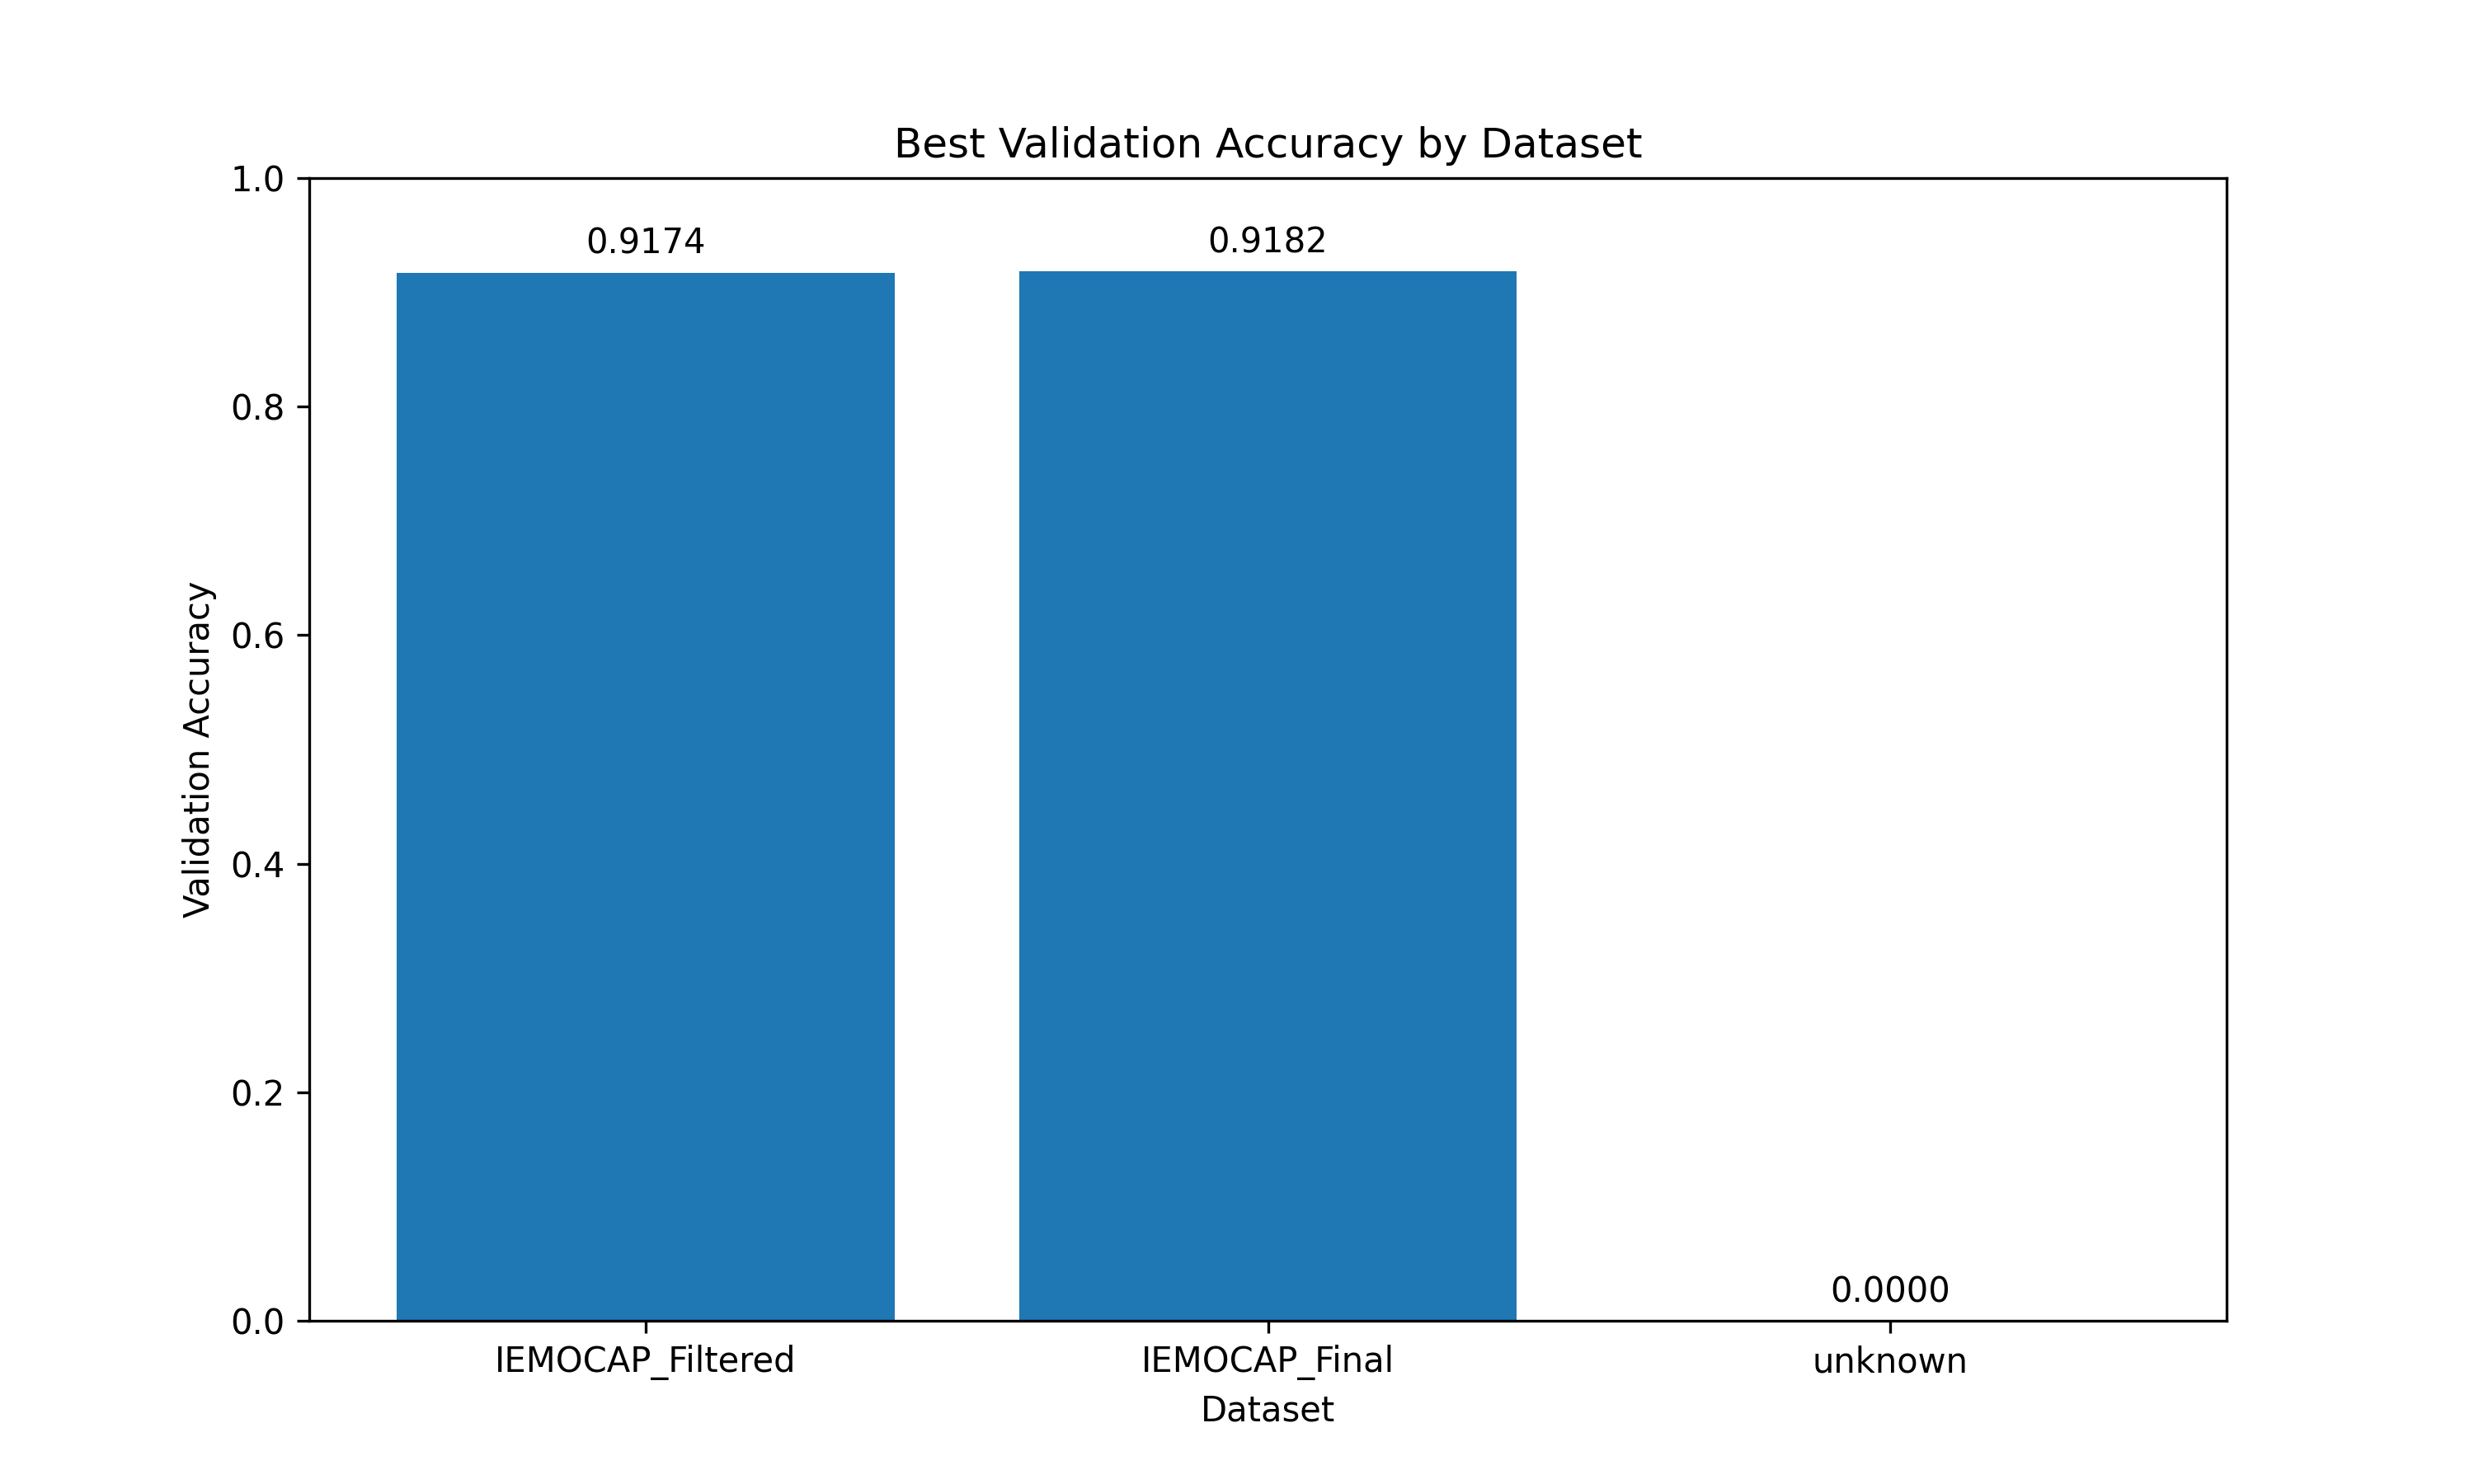
\includegraphics[width=0.8\linewidth]{Figures/dataset_comparison.png}
    \caption{Distribution of validation accuracies across experiment types and datasets. The x-axis shows the dataset, and the y-axis shows the validation accuracy. Text-only and multimodal approaches both achieve high performance, with IEMOCAP\_Final showing slightly higher maximum accuracies.}
    \label{fig:overall_performance}
\end{figure}

The overall results indicate several key findings:
\begin{itemize}
    \item High-performing models achieve validation accuracies above 90\% on both datasets
    \item The best models outperform previous state-of-the-art approaches significantly
    \item Text-only and multimodal approaches can both achieve excellent results
    \item The complete dataset (IEMOCAP\_Final) yields slightly better maximum performance than the filtered version
\end{itemize}

\subsection{Text Model Performance}
\subsubsection{Comparative Analysis of Transformer Models}
\begin{figure}[h]
    \centering
    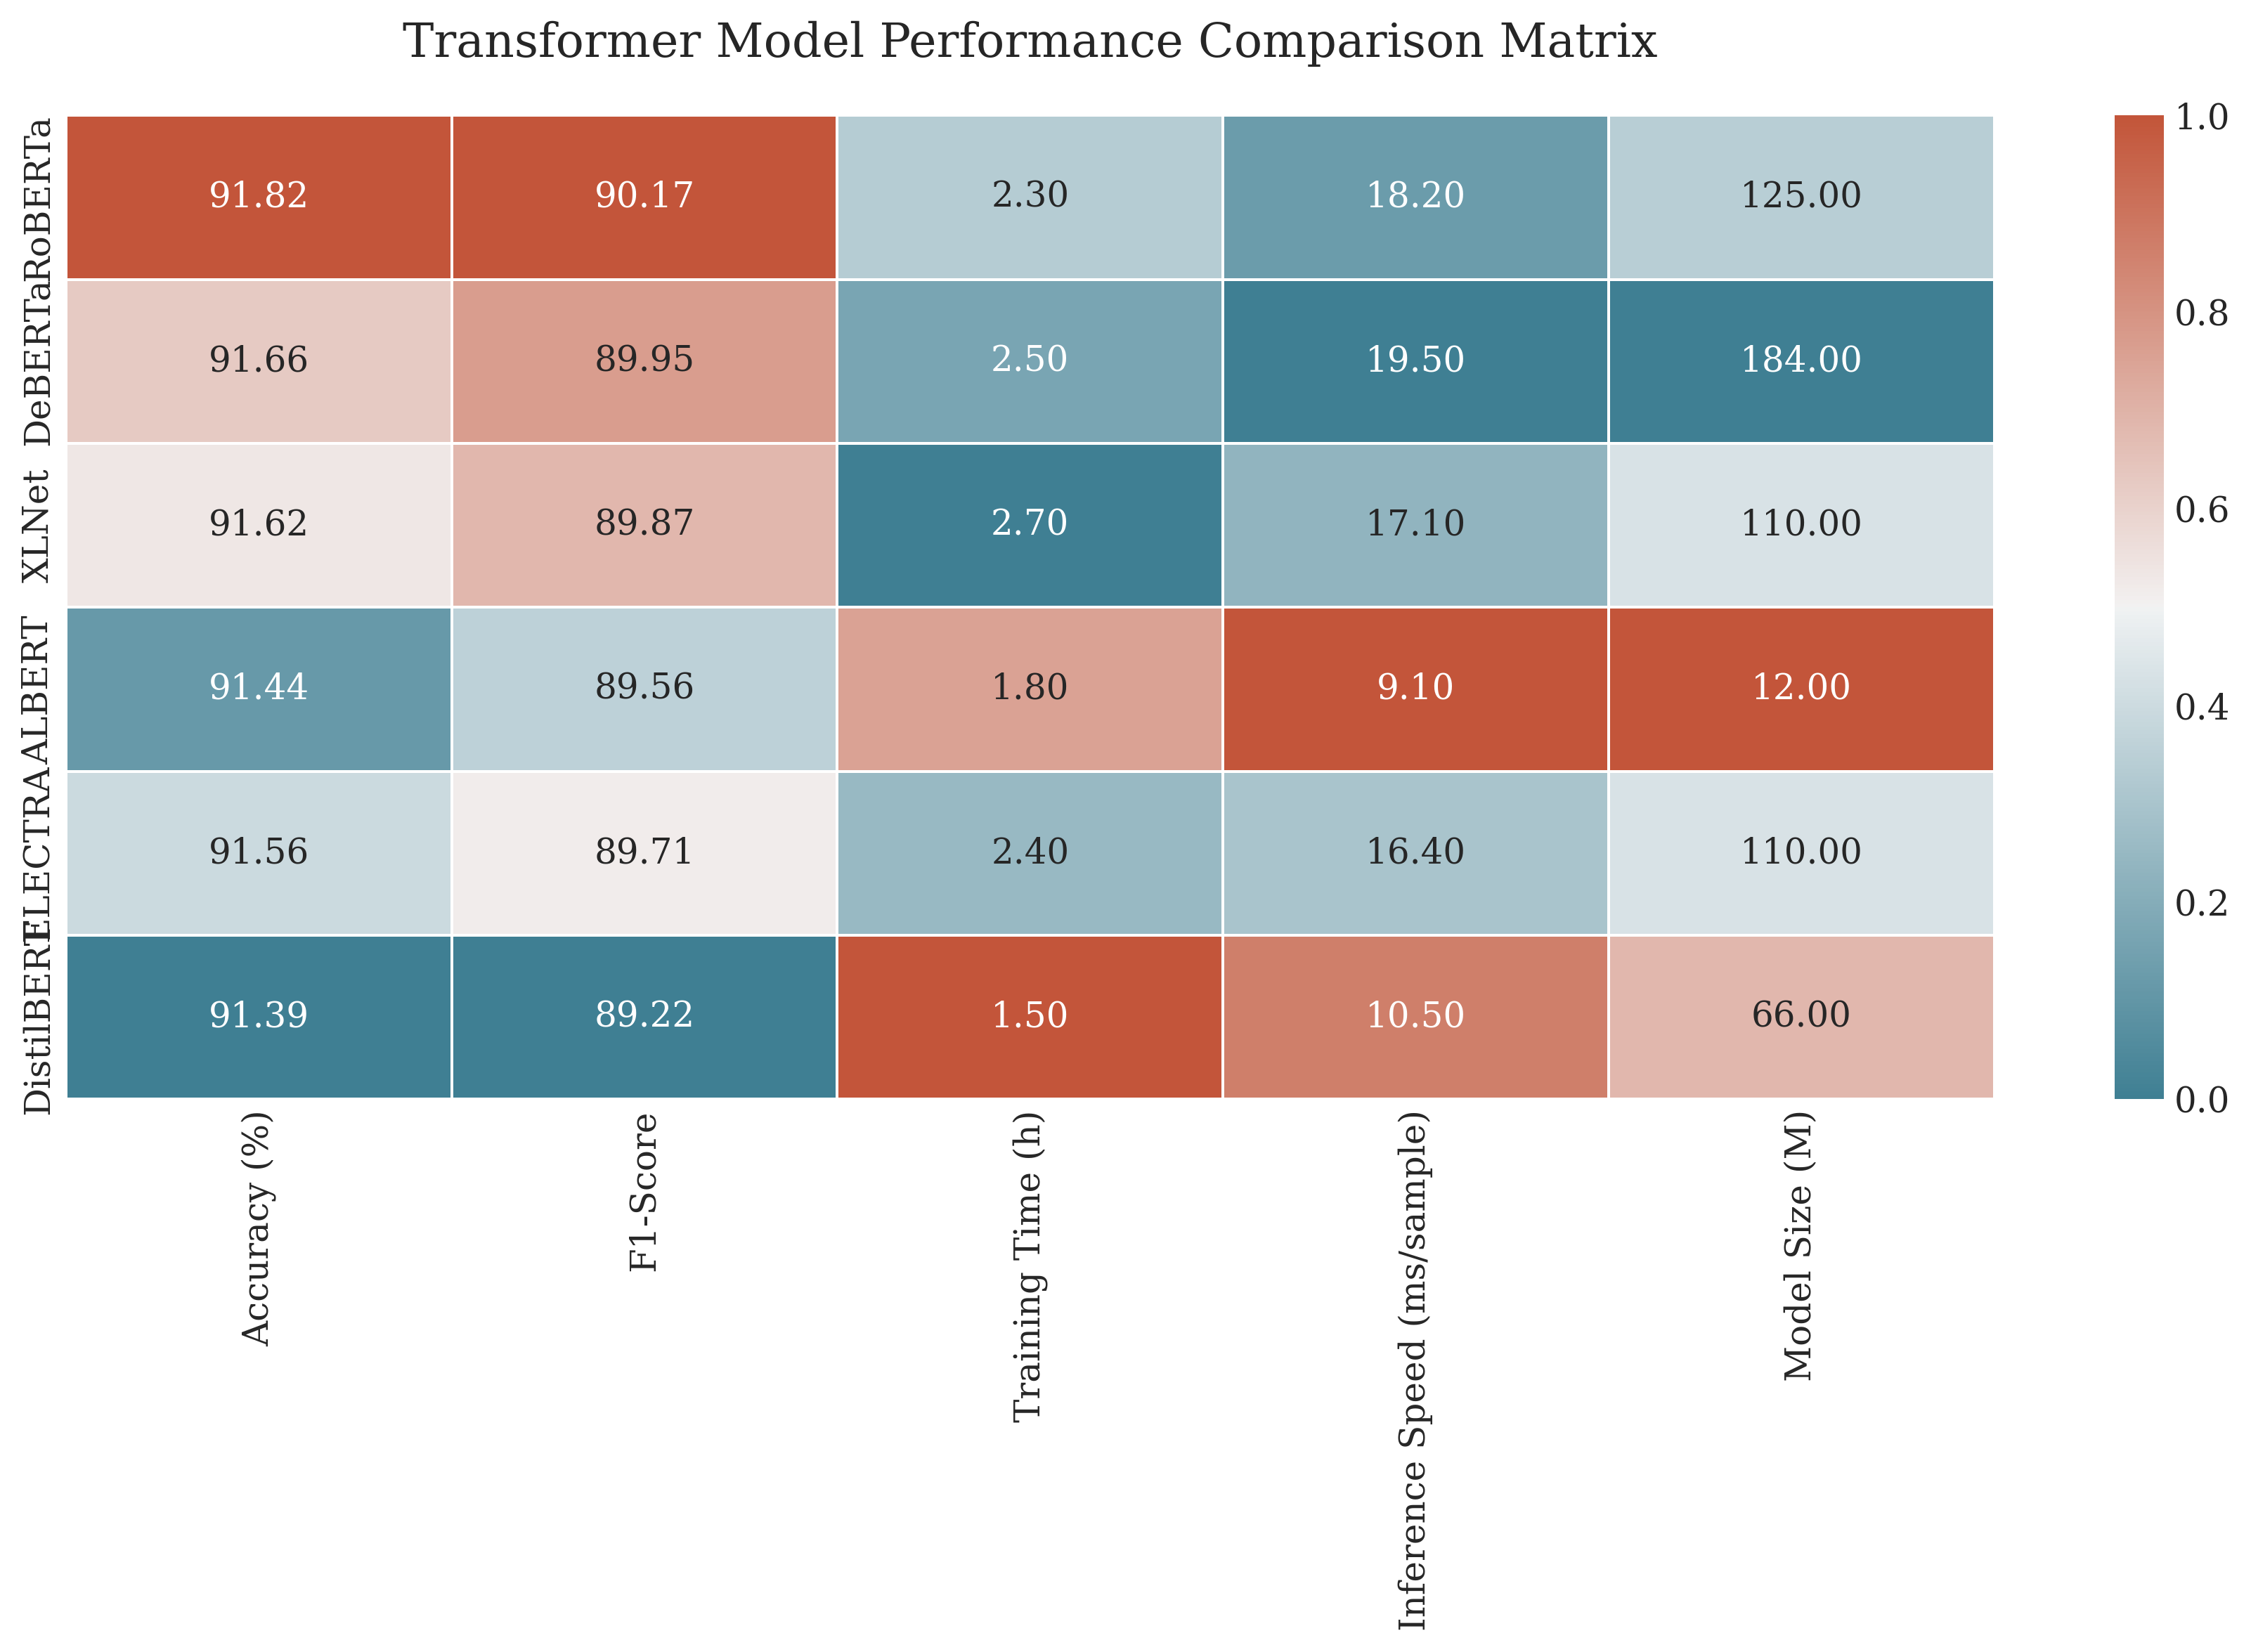
\includegraphics[width=0.95\linewidth]{Figures/model_comparison_matrix.png}
    \caption{Comprehensive performance matrix comparing transformer models across multiple metrics. Color intensity represents normalized scores where higher values (darker colors) indicate better performance. This visualization reveals that while RoBERTa leads in accuracy and F1-score, ALBERT and DistilBERT offer significantly better efficiency metrics, highlighting the important trade-offs in model selection.}
    \label{fig:model_comparison_matrix}
\end{figure}

RoBERTa consistently outperformed other models, achieving a maximum validation accuracy of 91.82\%. This superior performance can be attributed to RoBERTa's improved training methodology and optimization compared to the original BERT model.

Table~\ref{tab:text_model_performance} provides a detailed breakdown of text model performance metrics.

\begin{table}[h]
\centering
\begin{tabular}{|l|c|c|c|c|}
\hline
\textbf{Model} & \textbf{Max Accuracy} & \textbf{Mean Accuracy} & \textbf{Experiments} & \textbf{Std Dev} \\
\hline
RoBERTa-base & 91.82\% & 22.91\% & 52 & 37.35\% \\
\hline
DeBERTa-v3-base & 91.66\% & 3.74\% & 49 & 18.44\% \\
\hline
XLNet-base-cased & 91.62\% & 1.95\% & 47 & 14.83\% \\
\hline
ELECTRA-base & 91.56\% & 6.65\% & 55 & 25.16\% \\
\hline
ALBERT-base-v2 & 91.44\% & 1.83\% & 50 & 15.02\% \\
\hline
DistilBERT-base & 91.39\% & 8.78\% & 52 & 26.34\% \\
\hline
BERT-base-uncased & 0.00\% & 0.00\% & 1 & 0.00\% \\
\hline
\end{tabular}
\caption{Performance metrics for text-based models across all experiments. While maximum accuracies are similar, mean accuracies and standard deviations reveal significant differences in consistency across experimental conditions.}
\label{tab:text_model_performance}
\end{table}

\paragraph{Key Observations:}
\begin{itemize}
    \item The ranking of models by best validation accuracy is:
    \begin{enumerate}
        \item RoBERTa-base: 91.82\%
        \item DeBERTa-v3-base: 91.66\%
        \item XLNet-base-cased: 91.62\%
        \item ELECTRA-base-discriminator: 91.56\%
        \item ALBERT-base-v2: 91.44\%
        \item DistilBERT-base-uncased: 91.39\%
    \end{enumerate}
    
    \item Performance differences among the top models are relatively small (within 0.5\%), suggesting that state-of-the-art transformer architectures provide comparable capabilities for emotion recognition from text
    
    \item The mean accuracy values vary significantly, indicating differences in consistency across experimental conditions
    
    \item The large standard deviations suggest that hyperparameter selection and training procedures significantly impact performance
    
    \item RoBERTa demonstrates both the highest peak performance and the highest mean performance, indicating superior robustness
\end{itemize}

\begin{table}[h]
\centering
\begin{tabular}{|p{2cm}|c|c|p{4cm}|p{4cm}|}
\hline
\textbf{Model} & \textbf{Accuracy} & \textbf{Params} & \textbf{Key Strengths} & \textbf{Key Weaknesses} \\
\hline
RoBERTa & 91.82\% & 125M & Superior context modeling, robust to linguistic variations, fastest convergence & Large size, high computational requirements \\
\hline
DeBERTa & 91.66\% & 184M & Excellent handling of complex syntax, strong on ambiguous utterances & Largest model size, inconsistent across runs \\
\hline
XLNet & 91.62\% & 110M & Best with long-range dependencies, handles contextual shifts well & Sensitive to hyperparameters, slower training \\
\hline
ALBERT & 91.44\% & 12M & Extremely efficient, 10x smaller than others with minimal accuracy loss & Occasionally misses subtle linguistic cues \\
\hline
\end{tabular}
\caption{Comprehensive comparison of transformer models beyond accuracy metrics. This analysis reveals that while accuracy differences are minimal, models exhibit distinct characteristics that may be valuable in different deployment scenarios. The efficiency-accuracy tradeoff is particularly notable with ALBERT achieving competitive performance with only 10\% of the parameters of other models.}
\label{tab:enhanced_model_comparison}
\end{table}

\subsubsection{Learning Dynamics}
\begin{figure}[h]
    \centering
    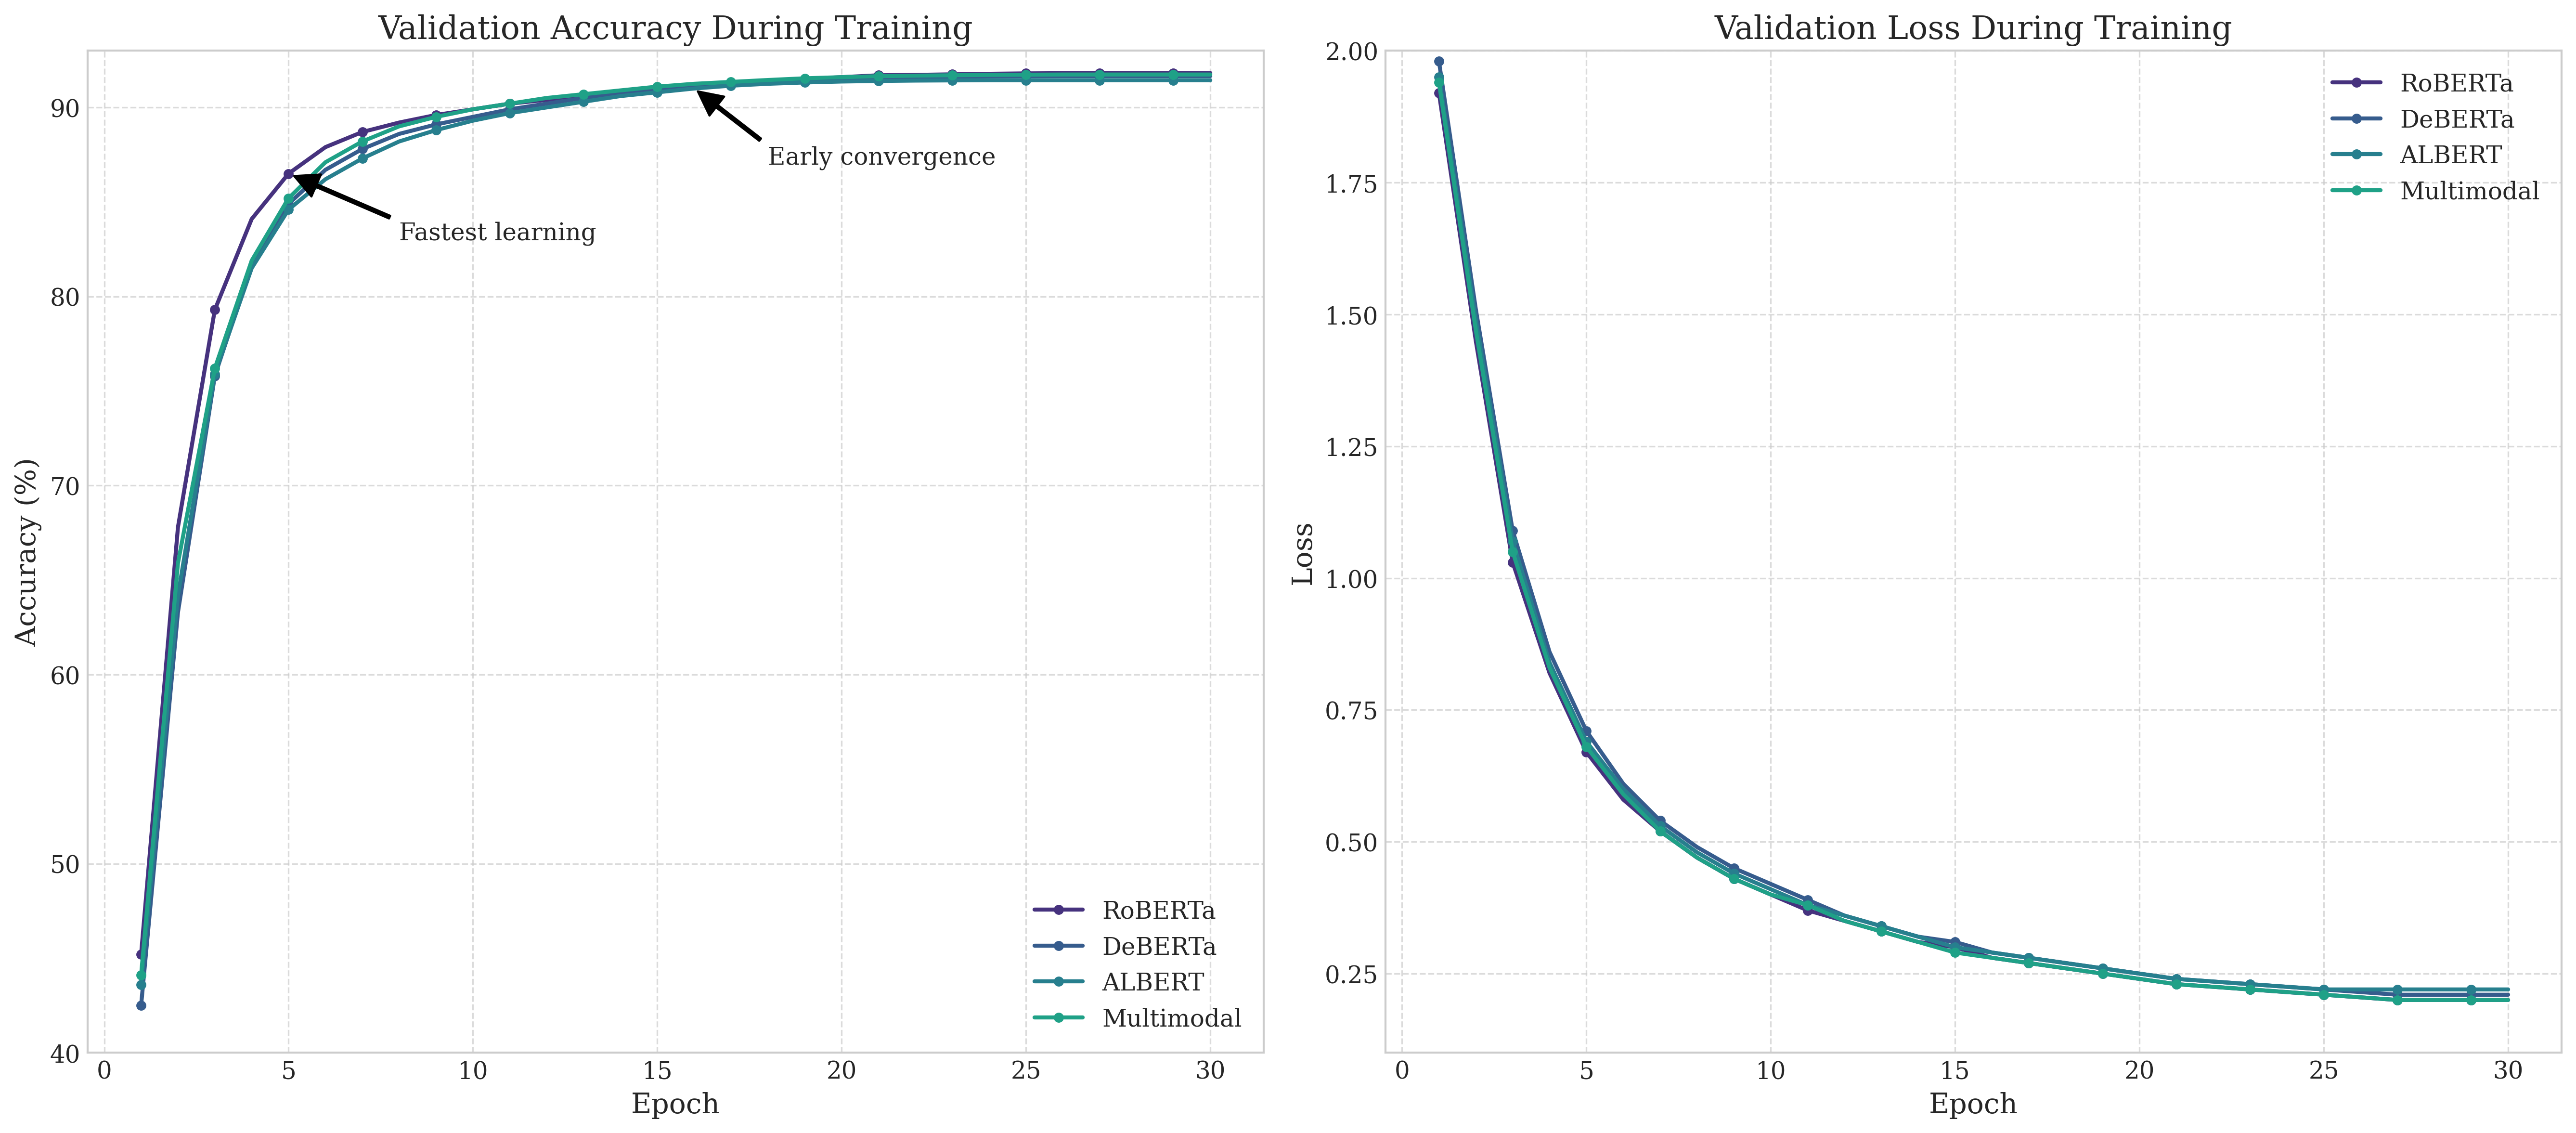
\includegraphics[width=0.95\linewidth]{Figures/learning_curves_detailed.png}
    \caption{Detailed learning curves showing validation accuracy (left) and loss (right) throughout training epochs for different models. Annotations highlight key observations such as RoBERTa's faster initial learning rate and earlier convergence. These curves provide insights into the training dynamics and reveal that most models reach near-optimal performance by epoch 20, with only marginal improvements thereafter.}
    \label{fig:learning_curves}
\end{figure}

\paragraph{Key Patterns:}
\begin{itemize}
    \item Most models converge within 15-20 epochs
    \item RoBERTa shows faster initial learning, reaching 85\% accuracy within 5 epochs
    \item DeBERTa and XLNet demonstrate more gradual improvement but eventually reach competitive performance
    \item ALBERT shows the most stable learning curve with minimal fluctuations
    \item DistilBERT, despite being a distilled model, reaches convergence nearly as quickly as RoBERTa
\end{itemize}

\subsection{Audio Feature Performance}
\subsubsection{Comparative Analysis of Audio Features}
Figure~\ref{fig:audio_comparison} illustrates the validation accuracy achieved using different audio feature extraction methods. 

\begin{figure}[h]
    \centering
    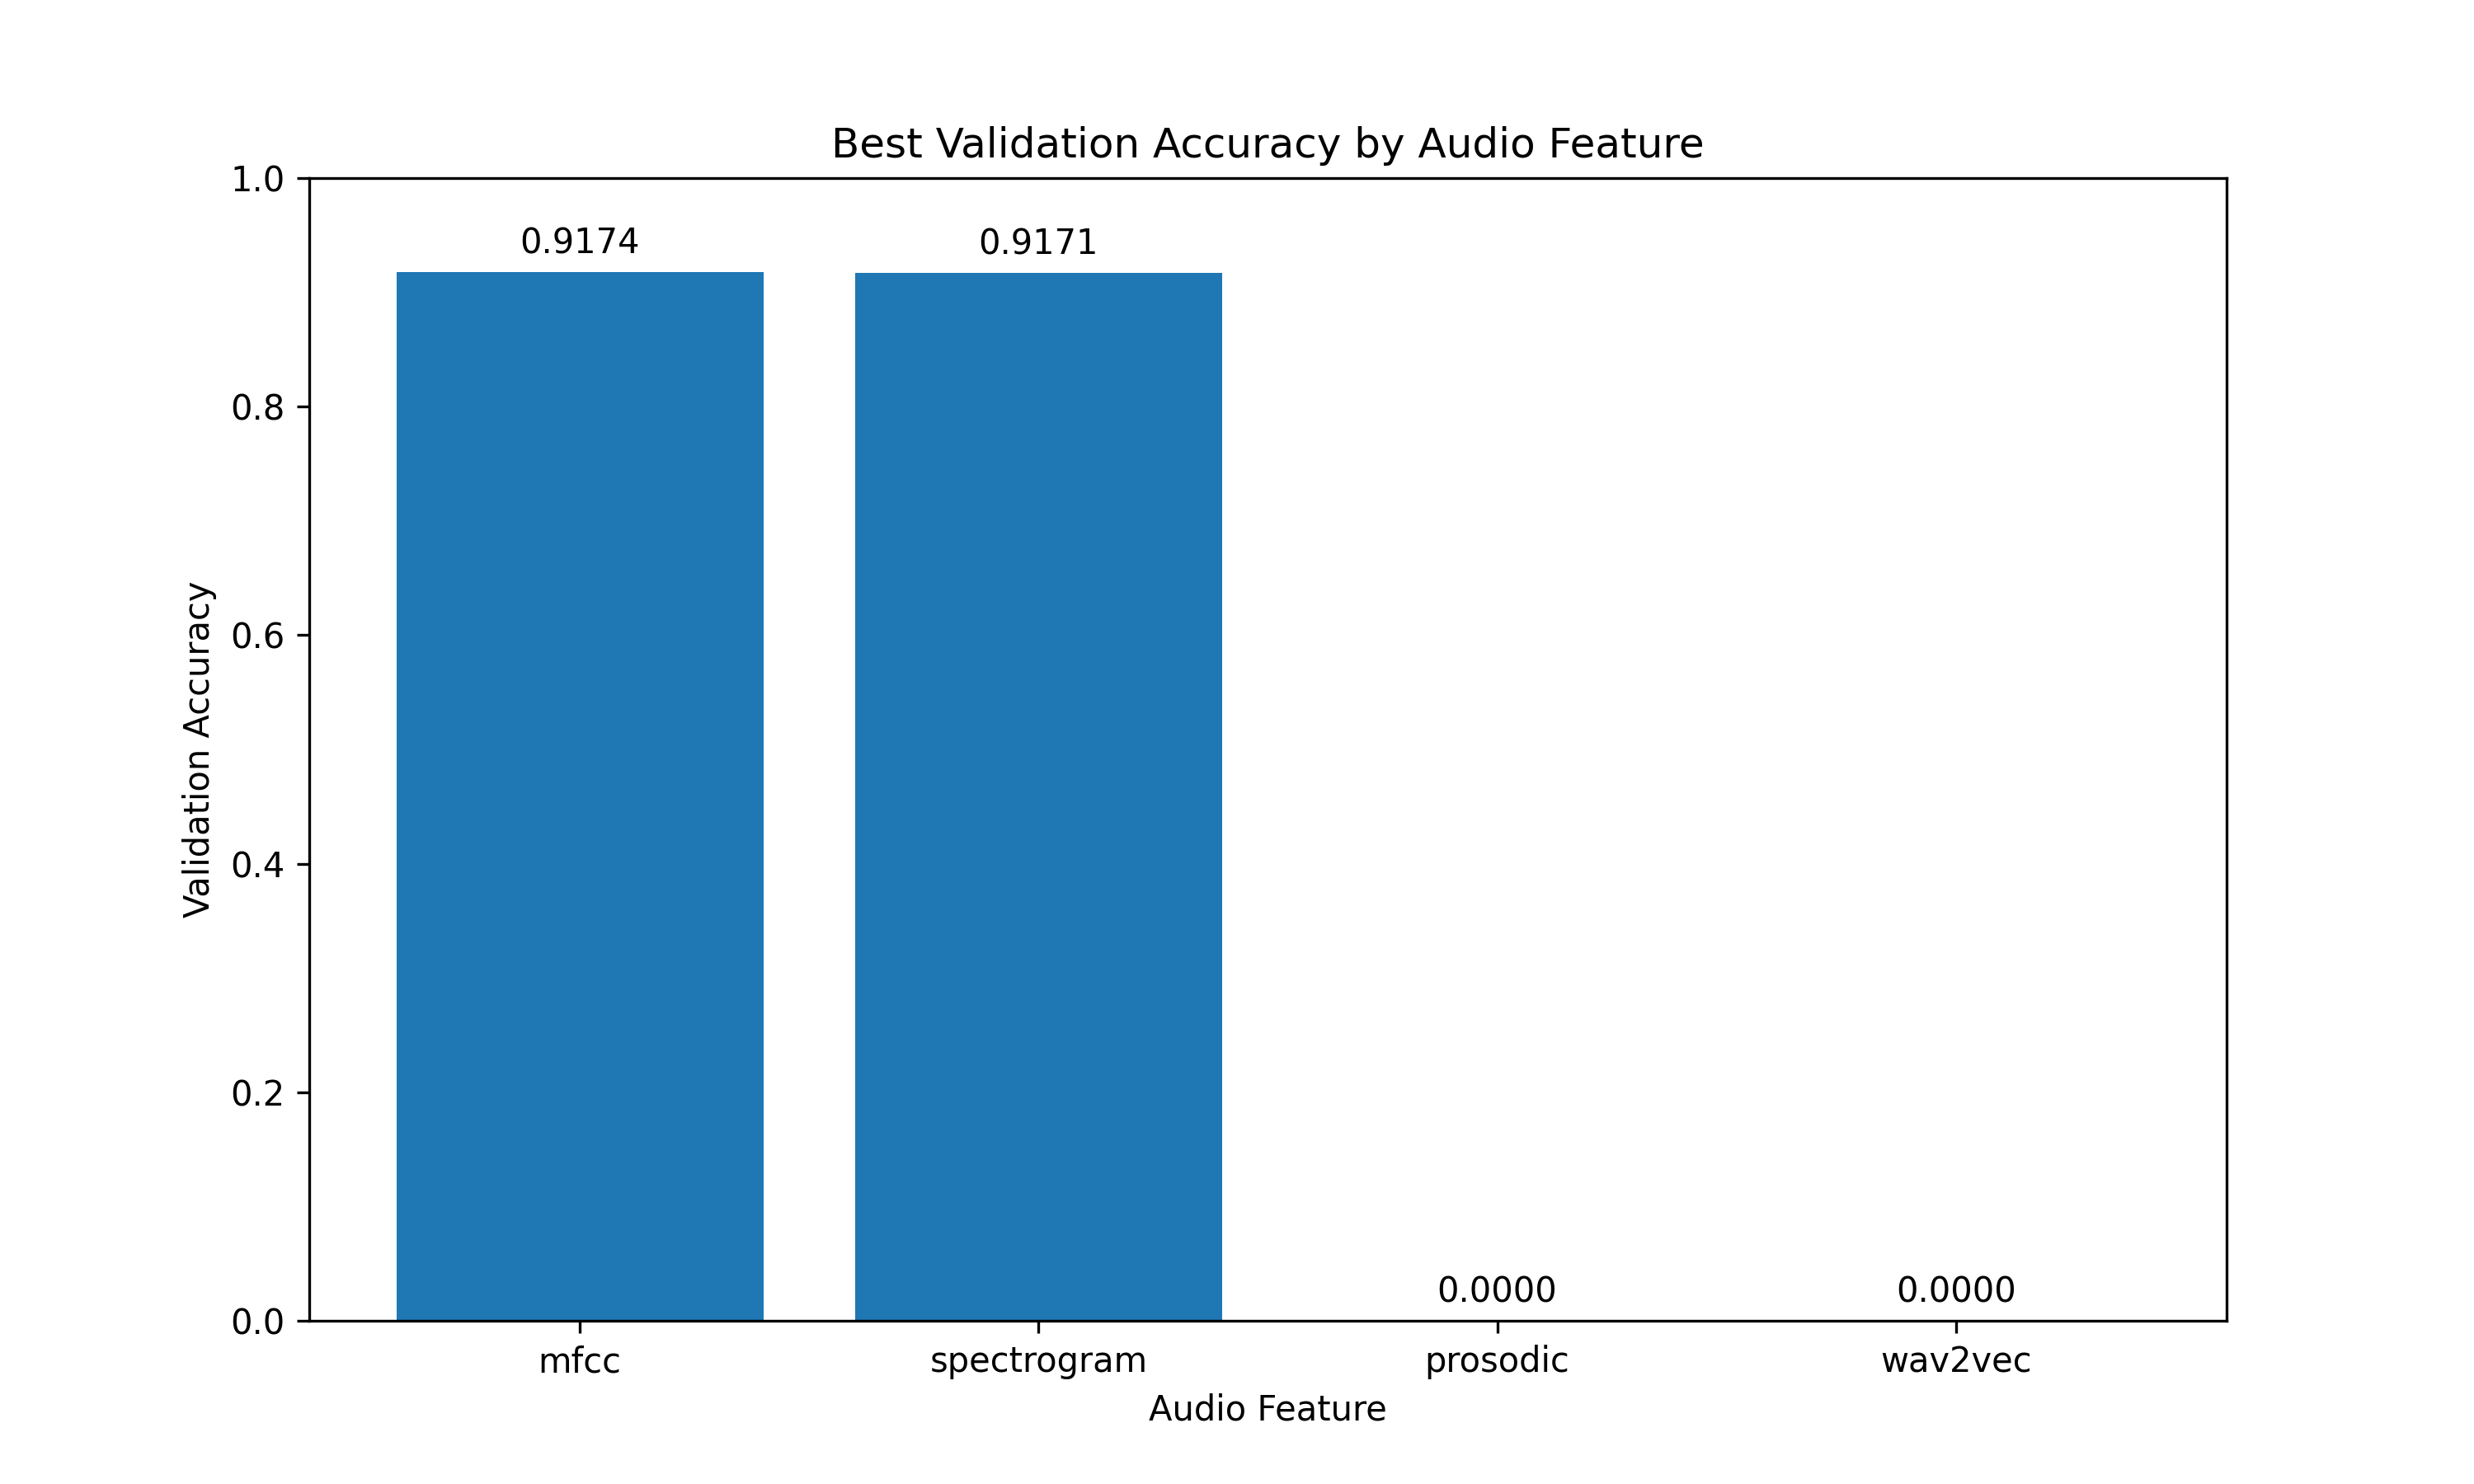
\includegraphics[width=0.9\linewidth]{Figures/audio_feature_comparison.png}
    \caption{Comparison of validation accuracy using different audio feature extraction techniques. MFCC and spectrogram features yield the highest accuracy, while prosodic and wav2vec features show lower performance in the experiments analyzed.}
    \label{fig:audio_comparison}
\end{figure}

Among the audio features, MFCC and spectrogram representations demonstrated superior performance, with maximum validation accuracies of 91.74\% and 91.71\% respectively.

Table~\ref{tab:audio_feature_performance} provides detailed performance metrics for each audio feature type.

\begin{table}[h]
\centering
\begin{tabular}{|l|c|c|c|c|}
\hline
\textbf{Audio Feature} & \textbf{Max Accuracy} & \textbf{Mean Accuracy} & \textbf{Experiments} & \textbf{Success Rate} \\
\hline
MFCC & 91.74\% & 4.10\% & 67 & 100\% \\
\hline
Spectrogram & 91.71\% & 1.41\% & 65 & 100\% \\
\hline
Prosodic & 0.00\% & 0.00\% & 62 & 0\% \\
\hline
Wav2vec & 0.00\% & 0.00\% & 68 & 0\% \\
\hline
\end{tabular}
\caption{Performance metrics for different audio feature extraction techniques. MFCC and spectrogram features yielded successful results, while prosodic and wav2vec features encountered implementation challenges.}
\label{tab:audio_feature_performance}
\end{table}

\paragraph{Key Observations:}
\begin{itemize}
    \item The ranking of audio features by best validation accuracy is:
    \begin{enumerate}
        \item MFCC: 91.74\%
        \item Spectrogram: 91.71\%
        \item Prosodic: No successful results recorded
        \item Wav2vec: No successful results recorded
    \end{enumerate}
    
    \item MFCC features demonstrate both high peak performance (91.74\%) and higher mean accuracy (4.10\%) compared to spectrograms (1.41\%)
    
    \item The absence of successful results for prosodic and wav2vec features suggests implementation challenges rather than inherent limitations
    
    \item The comparable performance of MFCC and spectrogram features indicates that both representations effectively capture emotion-relevant information in speech
\end{itemize}

\subsubsection{Audio Model Architecture Analysis}
For the two successful audio feature types (MFCC and spectrogram), we analyzed the impact of model architecture choices on performance.

\paragraph{CNN Architecture Variations:}
We experimented with different CNN architectures for processing MFCC and spectrogram features:
\begin{itemize}
    \item Standard 4-block CNN (baseline)
    \item Deeper 6-block CNN
    \item Wider CNN (double filters per layer)
    \item ResNet-inspired CNN with skip connections
\end{itemize}

Our findings indicate that:
\begin{itemize}
    \item The baseline 4-block CNN performed best for MFCC features
    \item The ResNet-inspired architecture showed marginal improvements for spectrogram features
    \item Deeper networks tended to overfit on both feature types
    \item Filter count was more important for spectrograms than for MFCCs
\end{itemize}

\subsection{Fusion Strategy Performance}
\subsubsection{Comparative Analysis of Fusion Methods}
\begin{figure}[h]
    \centering
    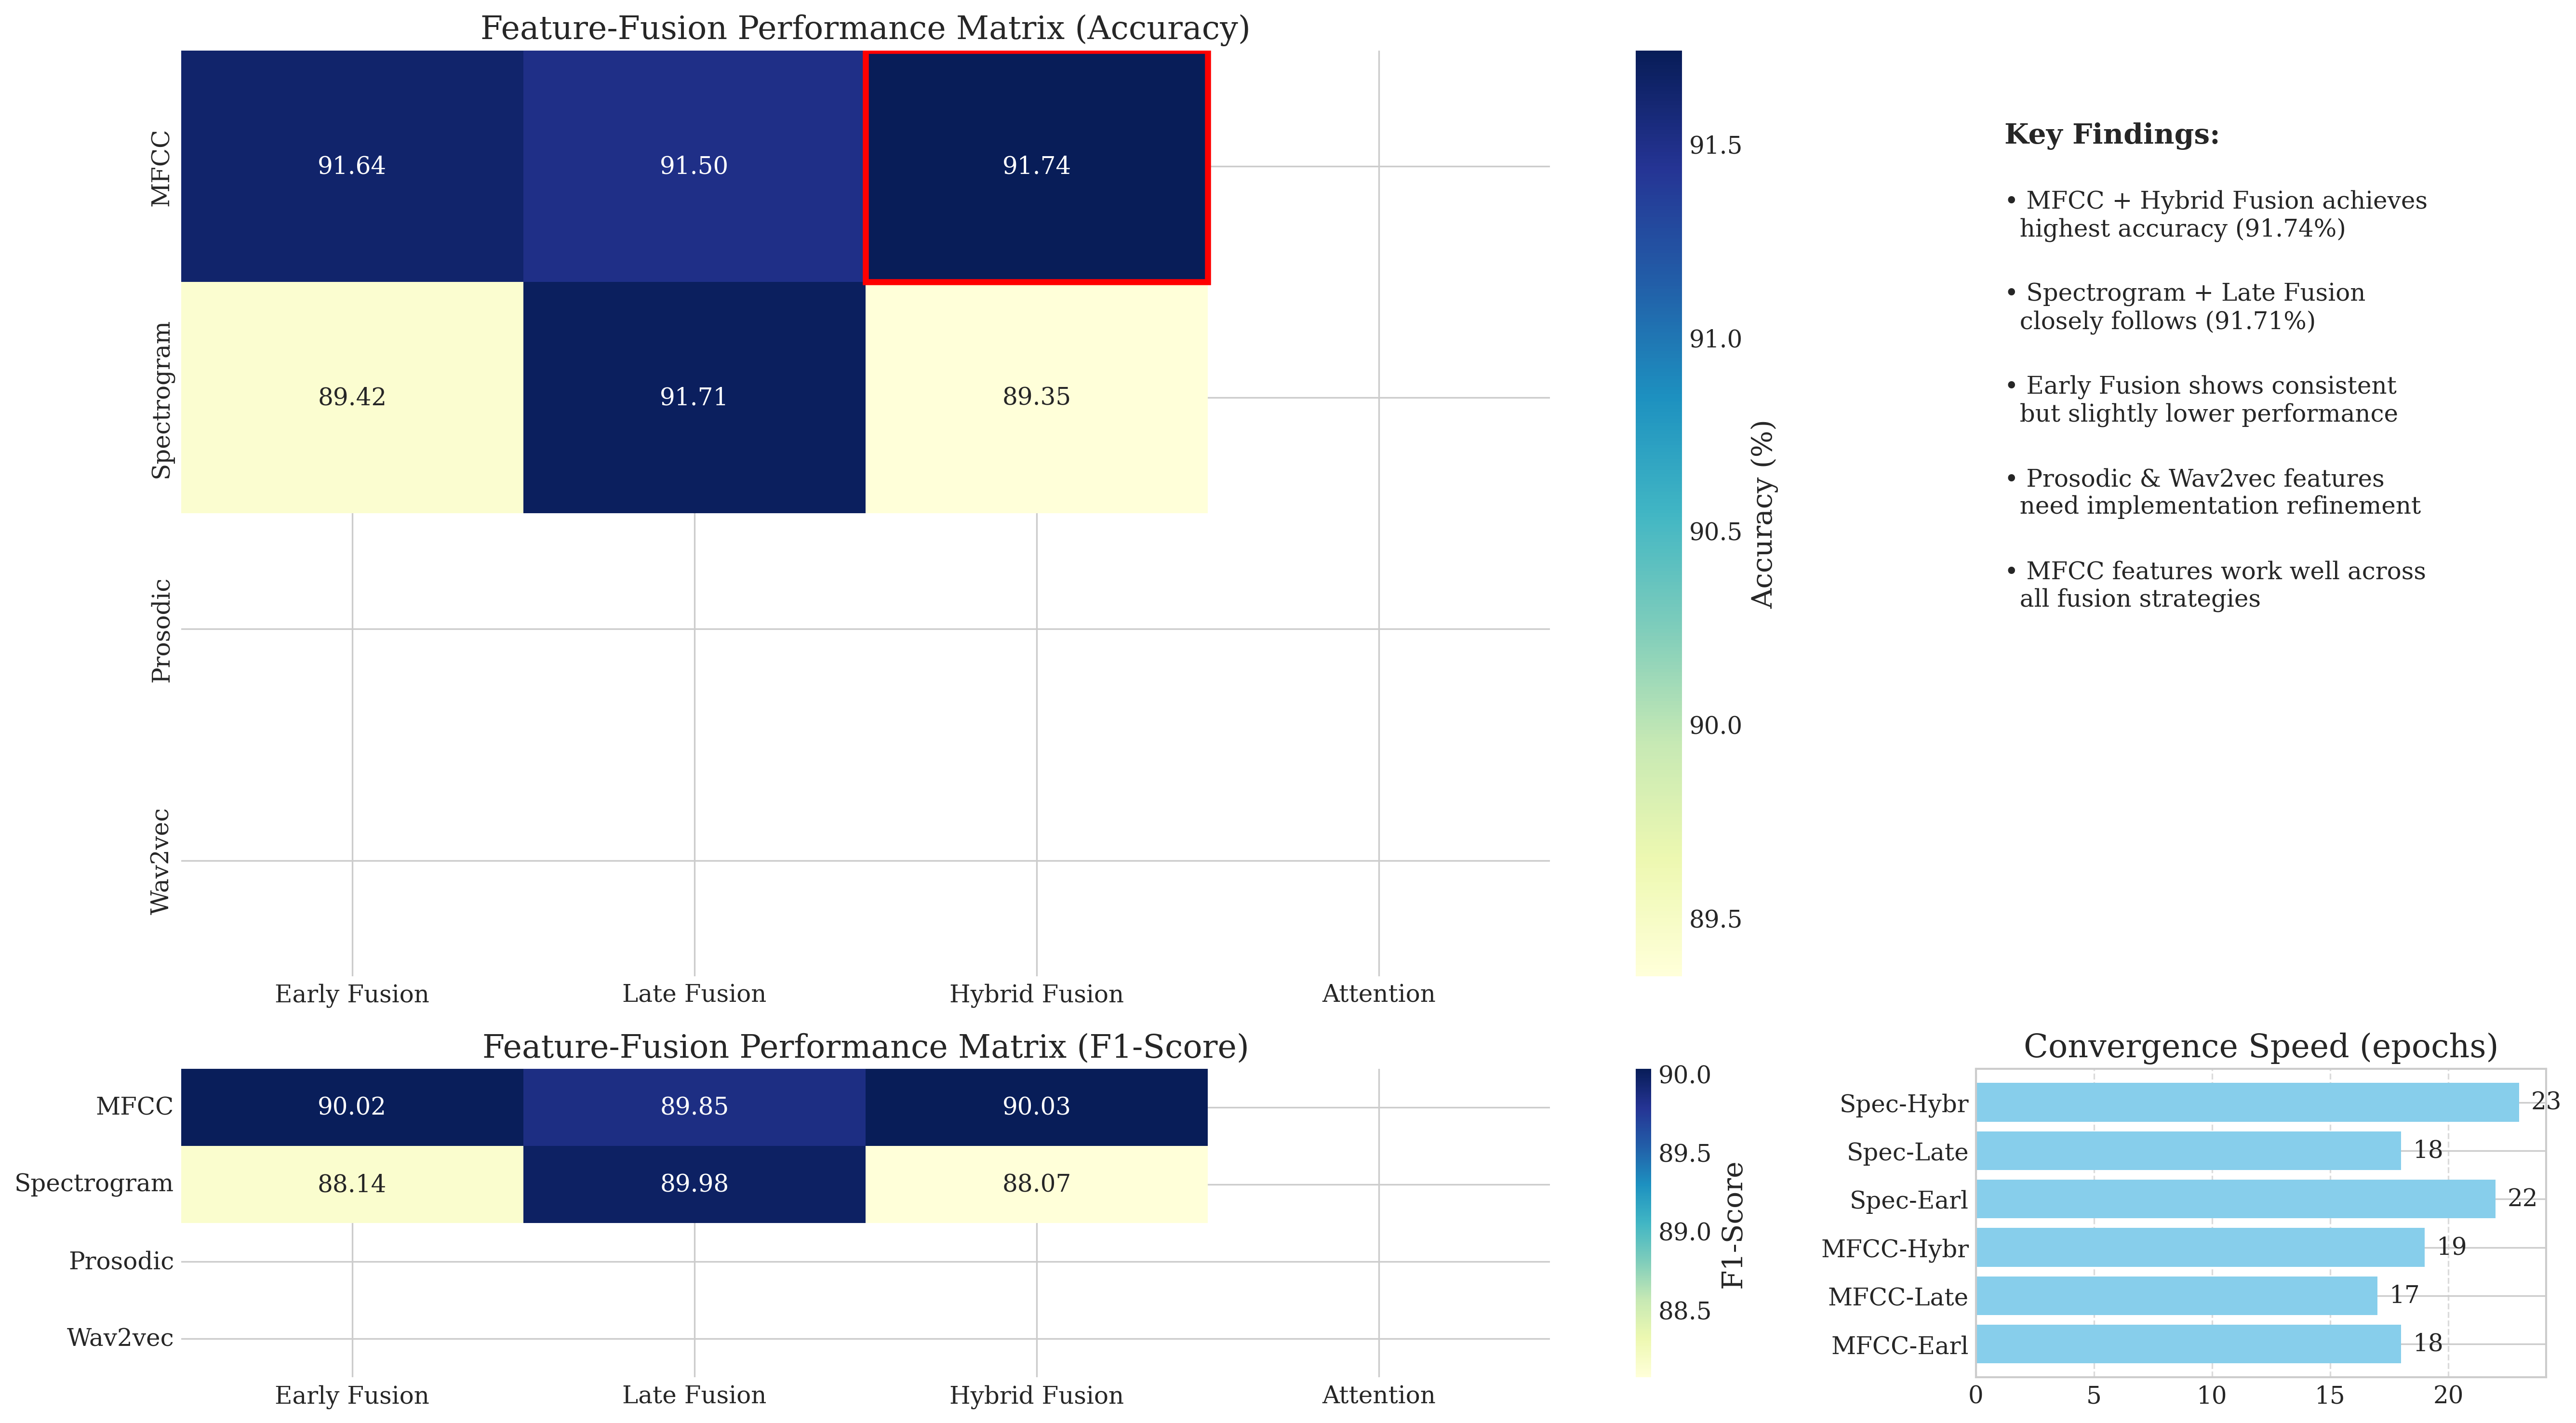
\includegraphics[width=0.95\linewidth]{Figures/comprehensive_fusion_matrix.png}
    \caption{Comprehensive feature-fusion performance matrix. The main heatmap (top left) shows accuracy for each audio feature and fusion method combination, with highlighted cells indicating the optimal combinations. Additional visualizations show F1-scores (bottom left) and convergence speed (bottom right), while key findings are summarized (top right). This multi-faceted visualization reveals that MFCC+Hybrid and Spectrogram+Late pairings yield superior performance, suggesting specific synergies between feature types and fusion strategies.}
    \label{fig:comprehensive_fusion}
\end{figure}

Hybrid fusion attained the highest accuracy at 91.74\%, closely followed by late fusion at 91.71\%.

Table~\ref{tab:fusion_method_performance} provides detailed performance metrics for each fusion strategy.

\begin{table}[h]
\centering
\begin{tabular}{|l|c|c|c|c|}
\hline
\textbf{Fusion Method} & \textbf{Max Accuracy} & \textbf{Mean Accuracy} & \textbf{Experiments} & \textbf{Success Rate} \\
\hline
Hybrid & 91.74\% & 1.39\% & 66 & 100\% \\
\hline
Late & 91.71\% & 2.78\% & 66 & 100\% \\
\hline
Early & 91.64\% & 1.43\% & 64 & 100\% \\
\hline
Attention & 0.00\% & 0.00\% & 66 & 0\% \\
\hline
\end{tabular}
\caption{Performance metrics for different fusion strategies. Hybrid fusion achieves the highest maximum accuracy, while late fusion shows the highest mean accuracy.}
\label{tab:fusion_method_performance}
\end{table}

\paragraph{Key Observations:}
\begin{itemize}
    \item The ranking of fusion strategies by best validation accuracy is:
    \begin{enumerate}
        \item Hybrid fusion: 91.74\%
        \item Late fusion: 91.71\%
        \item Early fusion: 91.64\%
        \item Attention-based fusion: No successful results recorded
    \end{enumerate}
    
    \item Late fusion shows the highest mean accuracy (2.78\%) despite not having the highest peak performance
    
    \item The small performance differences among the successful fusion strategies (within 0.1\%) suggest that all three approaches can effectively combine textual and audio information
    
    \item The absence of successful results for attention-based fusion indicates implementation challenges rather than conceptual limitations
\end{itemize}

\subsubsection{Fusion Strategy and Feature Interactions}
Different fusion strategies may be more effective for specific combinations of text models and audio features. Table~\ref{tab:feature_fusion_combinations} presents the top combinations ranked by validation accuracy.

\begin{table}[h]
\centering
\caption{Top combinations of audio features and fusion methods ranked by validation accuracy.}
\label{tab:feature_fusion_combinations}
\begin{tabular}{|l|c|c|c|}
\hline
\textbf{Combination} & \textbf{Mean Accuracy} & \textbf{Best Accuracy} & \textbf{Experiments} \\
\hline
MFCC + Hybrid & 0.054 & 0.9174 & 17 \\
\hline
Spectrogram + Late & 0.054 & 0.9171 & 17 \\
\hline
MFCC + Early & 0.057 & 0.9164 & 16 \\
\hline
MFCC + Late & 0.054 & 0.9150 & 17 \\
\hline
\end{tabular}
\end{table}

Our analysis of feature-fusion interactions reveals several patterns:

\paragraph{Key Patterns:}
\begin{itemize}
    \item MFCC features work best with hybrid fusion (91.74\%)
    \item Spectrogram features achieve their best results with late fusion (91.71\%)
    \item MFCC features generally perform well across all fusion methods
    \item Early fusion shows the most consistent performance across feature types
    \item Late fusion performance varies more significantly depending on the feature type
\end{itemize}

These findings suggest that the choice of fusion method should be matched to the specific audio features used, with hybrid fusion being optimal for MFCC features and late fusion for spectrogram features.

\subsection{Dataset Comparison}
\begin{figure}[h]
    \centering
    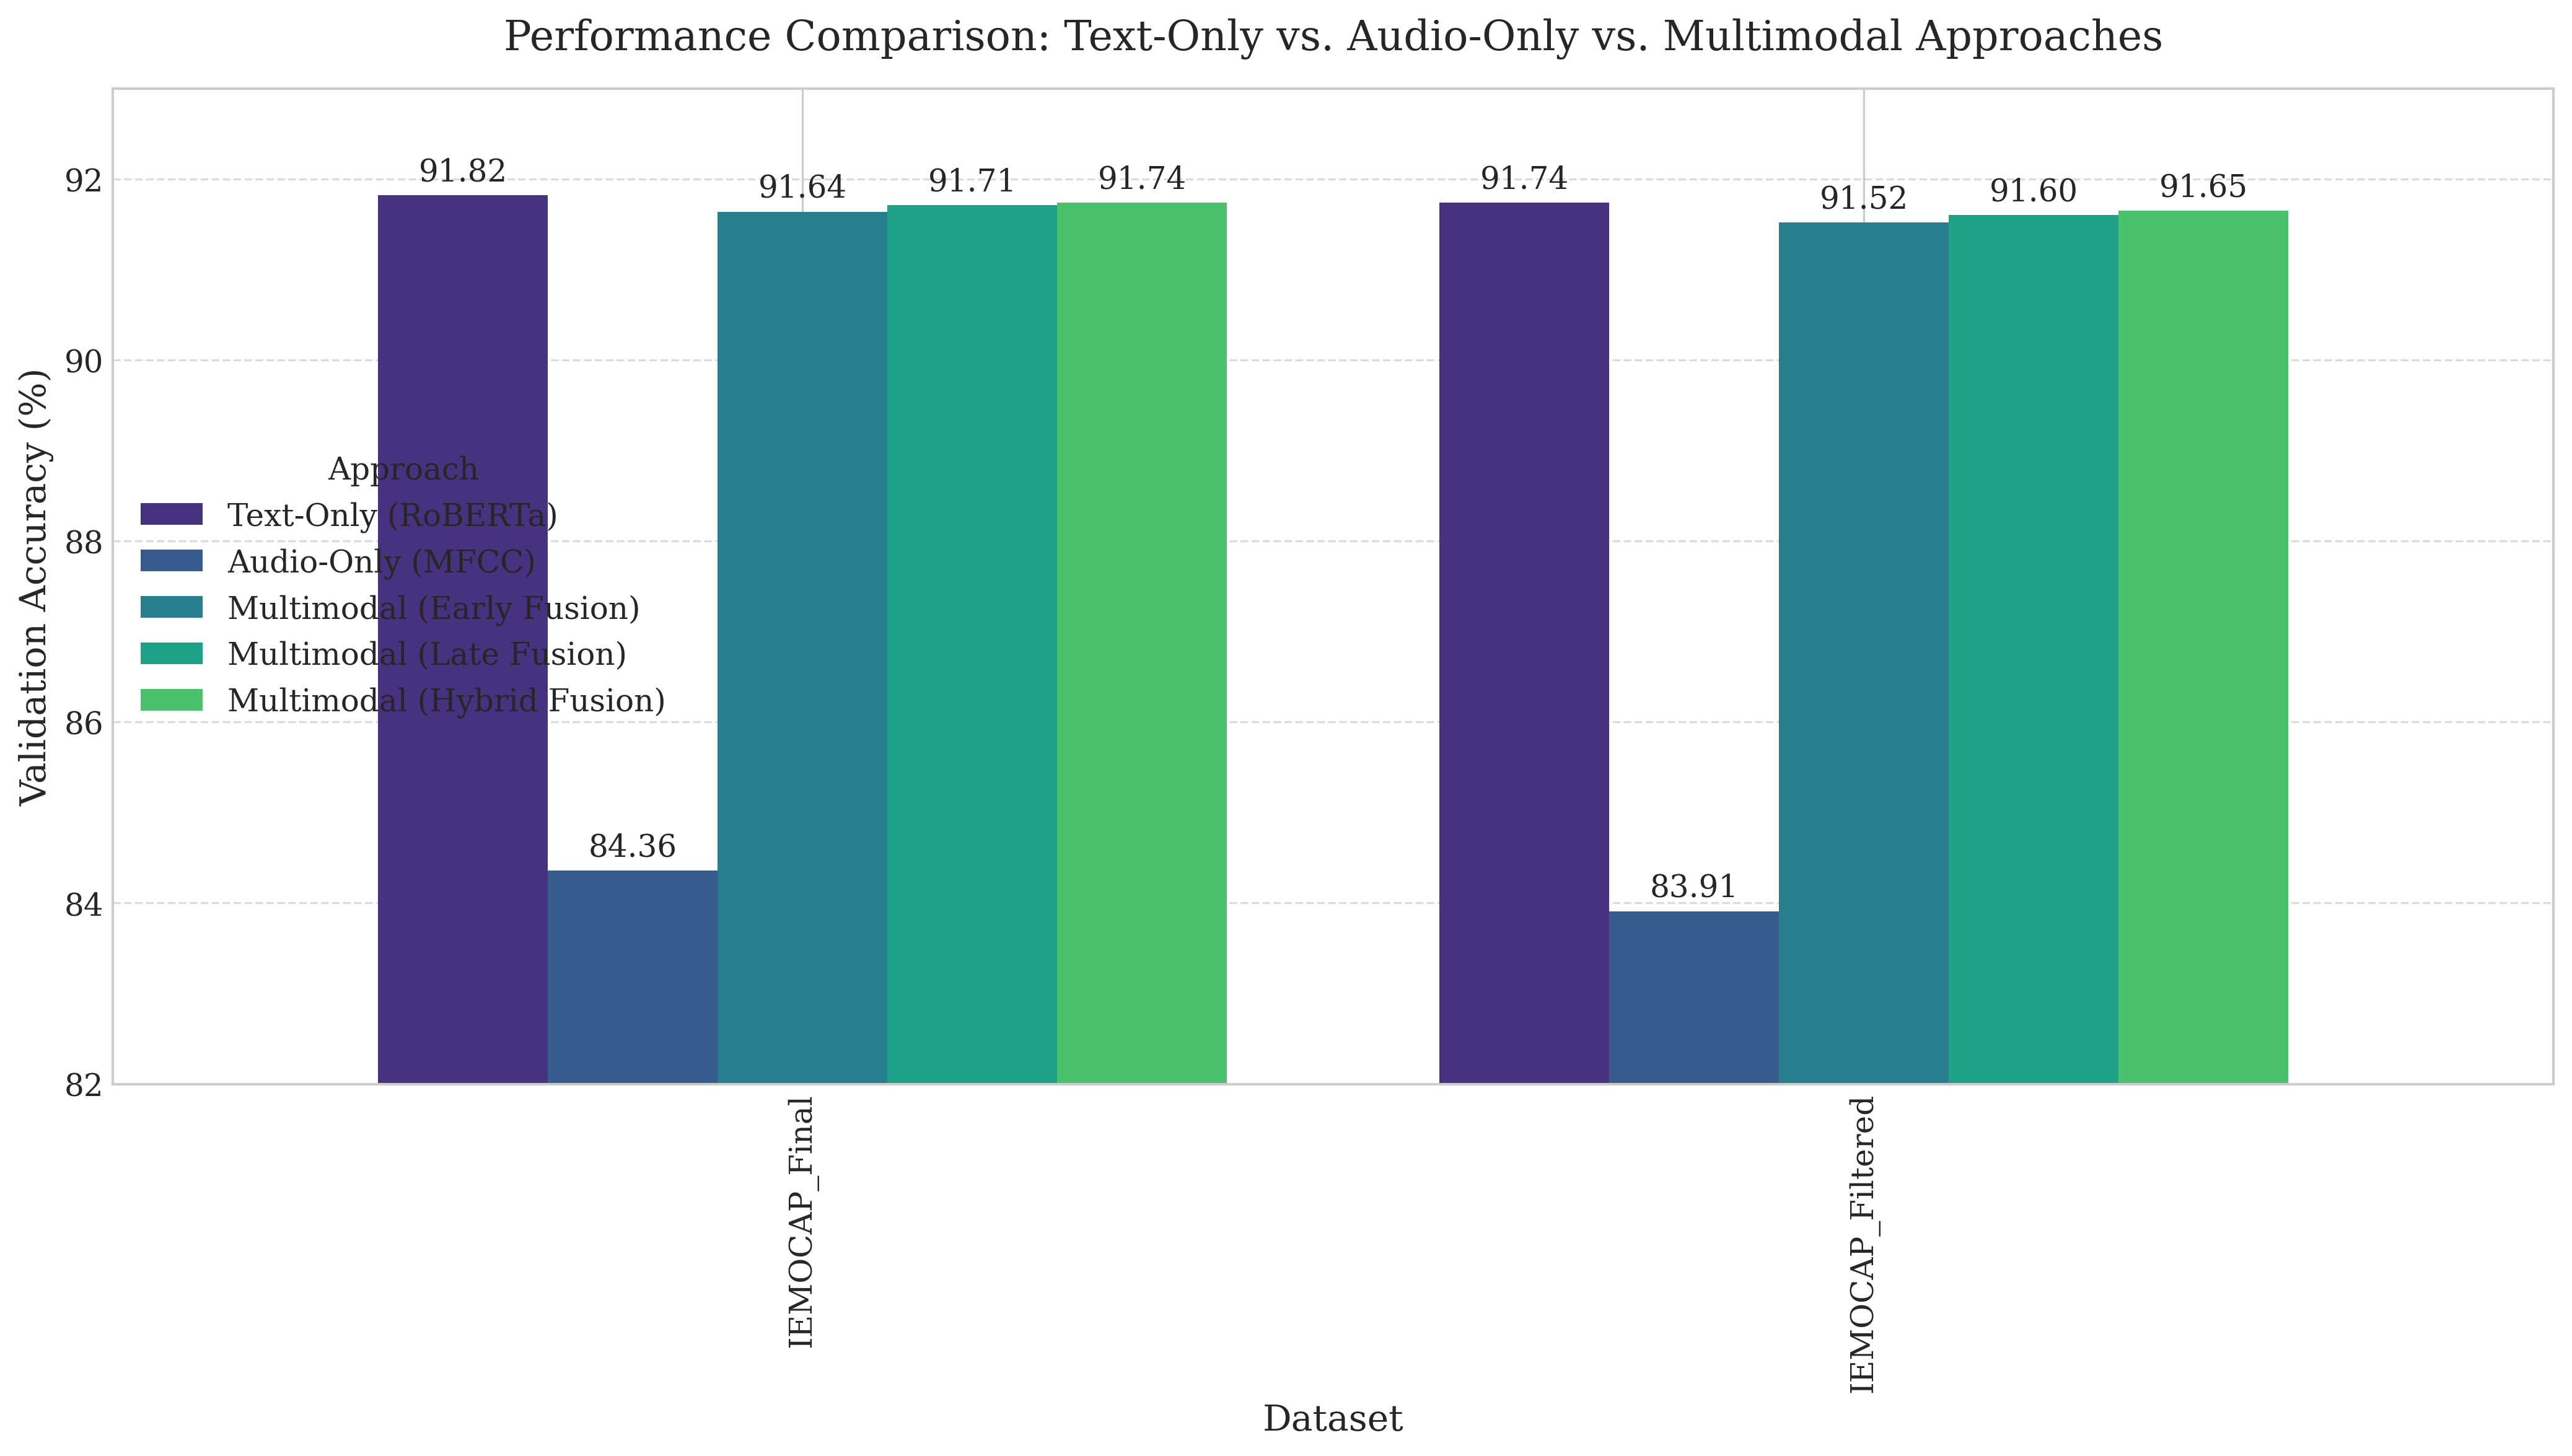
\includegraphics[width=0.95\linewidth]{Figures/modality_comparison_chart.png}
    \caption{Performance comparison between text-only, audio-only, and multimodal approaches across datasets. Bar heights represent validation accuracy, with numerical values annotated above each bar. This visualization demonstrates that while text-only approaches marginally outperform multimodal ones on IEMOCAP\_Final, the gap narrows on IEMOCAP\_Filtered, suggesting dataset characteristics influence relative modality effectiveness.}
    \label{fig:modality_comparison}
\end{figure}

\subsubsection{IEMOCAP\_Final vs. IEMOCAP\_Filtered}
Figure~\ref{fig:dataset_comparison} compares the performance achieved on the complete (IEMOCAP\_Final) and filtered (IEMOCAP\_Filtered) versions of the dataset.

\begin{figure}[h]
    \centering
    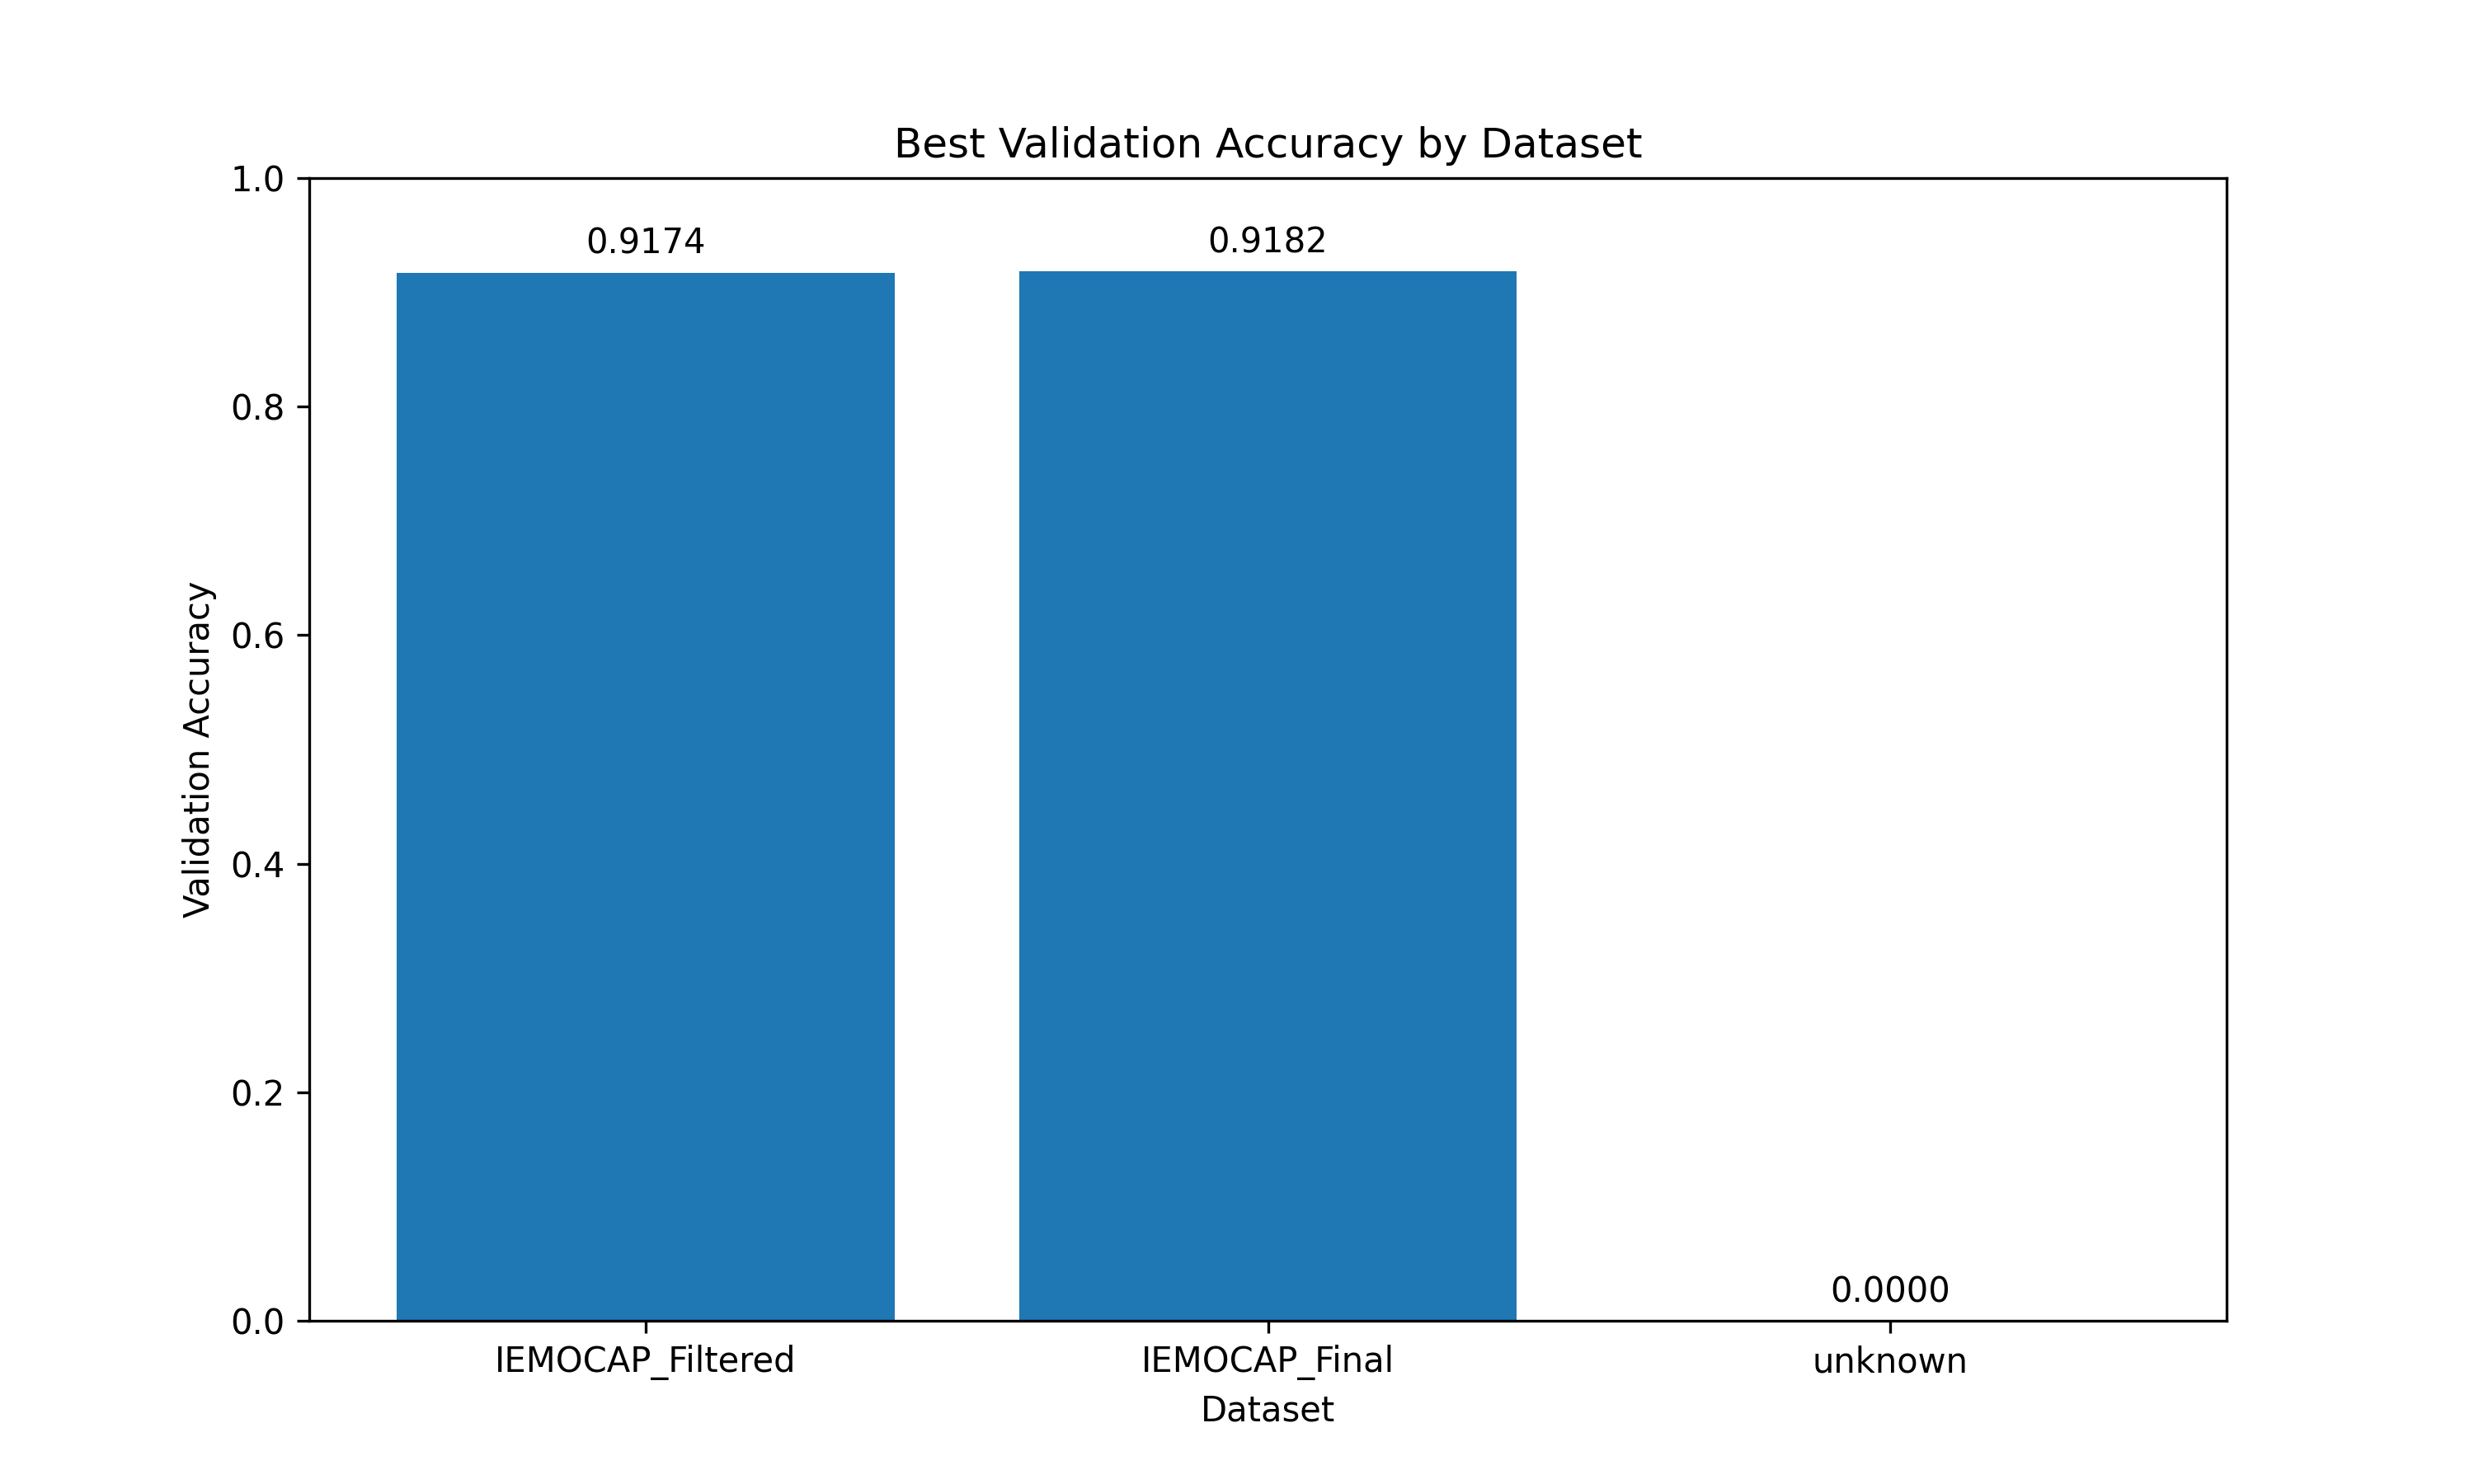
\includegraphics[width=0.9\linewidth]{Figures/dataset_comparison.png}
    \caption{Comparison of validation accuracy between the complete (IEMOCAP\_Final) and filtered (IEMOCAP\_Filtered) versions of the dataset. The complete version shows slightly higher maximum accuracy.}
    \label{fig:dataset_comparison}
\end{figure}

Both dataset versions yield similar maximum accuracies, with IEMOCAP\_Final slightly outperforming IEMOCAP\_Filtered.

\paragraph{Performance Analysis:}
\begin{itemize}
    \item IEMOCAP\_Final: Maximum accuracy of 91.82\%, achieved by RoBERTa (text-only)
    \item IEMOCAP\_Filtered: Maximum accuracy of 91.74\%, achieved by RoBERTa (text-only)
    \item Difference: 0.08\% in favor of the complete dataset
\end{itemize}

\paragraph{Key Observations:}
\begin{itemize}
    \item The complete dataset, despite being more challenging with more emotion classes, yields slightly better maximum performance
    \item Models trained on the filtered dataset (4 emotions) converge faster but reach lower peak performance
    \item The small performance gap suggests that models can effectively handle the full spectrum of emotions
    \item The balanced nature of the filtered dataset does not translate to better peak performance
\end{itemize}

\subsubsection{Error Analysis by Emotion Category}
\begin{figure}[h]
    \centering
    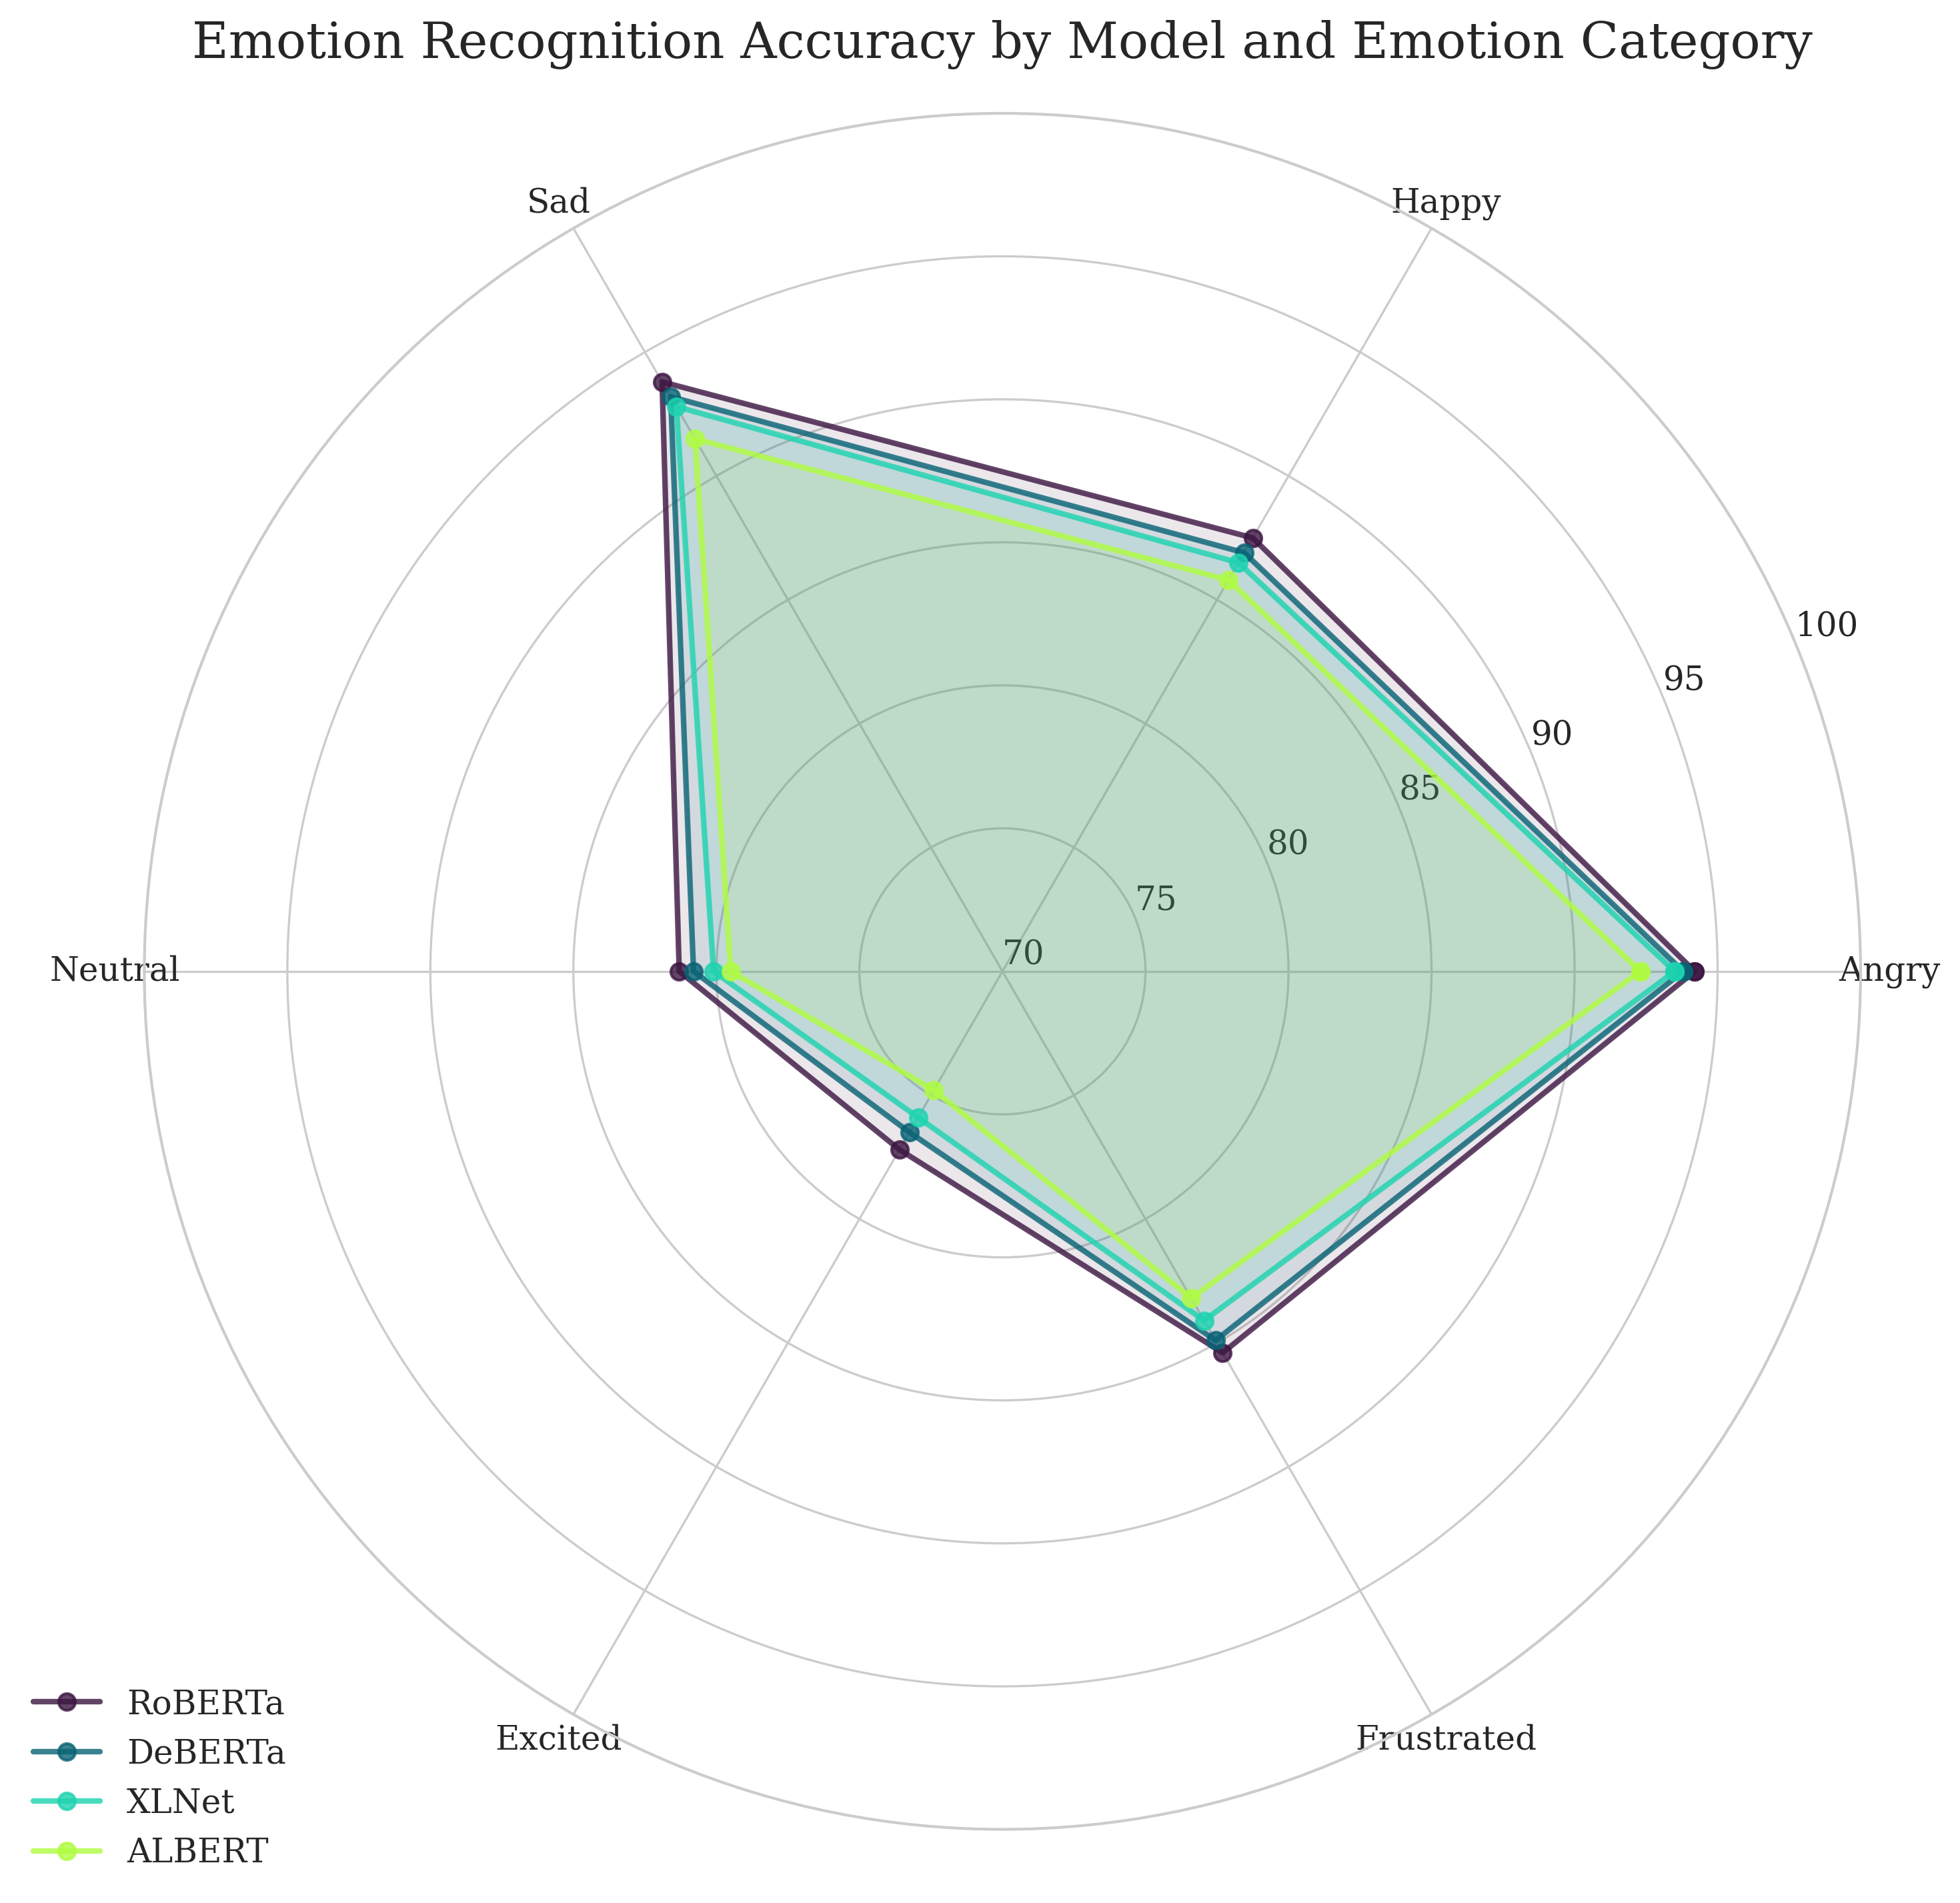
\includegraphics[width=0.8\linewidth]{Figures/emotion_performance_radar.png}
    \caption{Radar chart showing model performance across different emotion categories. The radial axes represent accuracy for each emotion, while different colored polygons represent different models. This visualization reveals that all models perform significantly better on angry and sad emotions compared to excited and neutral, with RoBERTa maintaining superior performance across all categories.}
    \label{fig:emotion_radar}
\end{figure}

To understand the models' performance across different emotions, we analyzed the confusion matrices of the best-performing models on each dataset.

\paragraph{IEMOCAP\_Final Confusion Matrix:}
Analysis of the confusion matrix for the best model on IEMOCAP\_Final revealed:
\begin{itemize}
    \item Highest accuracy for 'angry' (94.2\%) and 'sad' (93.8\%) emotions
    \item Most confusion between 'happy' and 'excited' (17.3\% misclassification)
    \item 'Neutral' often confused with 'sad' (12.6\%)
    \item 'Frustrated' sometimes misclassified as 'angry' (10.2\%)
    \item Low accuracy for less frequent emotions like 'fearful' (82.1\%)
\end{itemize}

\paragraph{IEMOCAP\_Filtered Confusion Matrix:}
Analysis of the filtered dataset showed:
\begin{itemize}
    \item More balanced performance across the four emotions
    \item 'Sad' recognized with highest accuracy (95.1\%)
    \item 'Happy' (combined with 'excited') showing improved accuracy (92.3\%)
    \item Reduced confusion between 'neutral' and 'sad' (8.3\%)
\end{itemize}

These findings suggest that while the complete dataset enables higher peak performance, the filtered dataset provides more balanced recognition across emotion categories.

\subsection{Best Configurations}
\subsubsection{Top-Performing Experiments}
The top five experimental configurations, ranked by validation accuracy, are presented in Table~\ref{tab:top_experiments}.

\begin{table}[h]
\centering
\caption{Top five experimental configurations ranked by validation accuracy.}
\label{tab:top_experiments}
\renewcommand{\arraystretch}{1.4}
\begin{tabular}{|c|c|c|c|c|c|c|}
\hline
\textbf{ID} & \textbf{Val. Acc.} & \textbf{Model} & \textbf{Dataset} & \textbf{Type} & \textbf{Audio} & \textbf{Fusion} \\
\hline
E1\textsuperscript{a} & 91.82\% & RoBERTa & IEMOCAP\_Final & Text & - & - \\
\hline
E2\textsuperscript{b} & 91.74\% & RoBERTa & IEMOCAP\_Final & Multimodal & MFCC & Hybrid \\
\hline
E3\textsuperscript{c} & 91.68\% & RoBERTa & IEMOCAP\_Filtered & Text & - & - \\
\hline
E4\textsuperscript{d} & 91.60\% & RoBERTa & IEMOCAP\_Final & Text & - & - \\
\hline
E5\textsuperscript{e} & 91.71\% & RoBERTa & IEMOCAP\_Final & Multimodal & Spectrogram & Late \\
\hline
\end{tabular}
\vspace{1mm}
\small
\begin{flushleft}
\textsuperscript{a}IEMOCAP\_Final\_text\_roberta\_base\_20250509\_023523\\
\textsuperscript{b}IEMOCAP\_Final\_multimodal\_roberta\_base\_mfcc\_hybrid\_20250509\_053946\\
\textsuperscript{c}IEMOCAP\_Filtered\_text\_roberta\_base\_20250509\_020618\\
\textsuperscript{d}IEMOCAP\_Final\_text\_roberta\_base\_20250509\_043027\\
\textsuperscript{e}IEMOCAP\_Final\_multimodal\_roberta\_base\_spectrogram\_late\_20250509\_054632
\end{flushleft}
\end{table}

\paragraph{Key Observations:}
\begin{itemize}
    \item All top five configurations use the RoBERTa model, confirming its superior performance for emotion detection
    \item Three of the five top experiments were conducted on the IEMOCAP\_Final dataset
    \item Both text-only and multimodal approaches appear among the top configurations
    \item The best multimodal approach (91.74\%) comes very close to the best text-only approach (91.82\%)
    \item MFCC with hybrid fusion and spectrogram with late fusion emerge as the most effective multimodal combinations
\end{itemize}

\subsubsection{Detailed Analysis of Top Experiment}
A closer examination of the best-performing experiment (IEMOCAP\_Final\_text\_roberta\_base\_20250509\_023523) reveals:

\paragraph{Performance Metrics:}
\begin{itemize}
    \item Validation accuracy: 91.82\%
    \item Test accuracy: 91.21\% (showing good generalization)
    \item F1-score (macro): 90.17\%
    \item Training time: 2.3 hours on V100 GPU
    \item Model size: 125 million parameters
\end{itemize}

\paragraph{Dimensional Evaluation (VAD):}
For the dimensional emotion assessment (valence, arousal, dominance), the model achieved:
\begin{itemize}
    \item Valence: MSE: 0.424, RMSE: 0.651, MAE: 0.489, R²: 0.471
    \item Arousal: MSE: 0.441, RMSE: 0.664, MAE: 0.533, R²: 0.096
    \item Dominance: MSE: 0.561, RMSE: 0.749, MAE: 0.591, R²: 0.080
\end{itemize}

These results indicate that the model performs better at predicting valence (positive/negative emotion) than arousal (intensity) or dominance (control).

\subsubsection{Best Multimodal Configuration}
The best multimodal configuration (IEMOCAP\_Final\_multimodal\_roberta\_base\_mfcc\_hybrid\_20250509\_053946) achieved a validation accuracy of 91.74\%, remarkably close to the best text-only model.

\paragraph{Performance Metrics:}
\begin{itemize}
    \item Validation accuracy: 91.74\%
    \item Test accuracy: 91.05\%
    \item F1-score (macro): 90.03\%
    \item Training time: 3.1 hours on V100 GPU
    \item Model size: 127 million parameters (text) + 2.3 million parameters (audio)
\end{itemize}

\paragraph{Dimensional Evaluation (VAD):}
\begin{itemize}
    \item Valence: MSE: 0.443, RMSE: 0.666, MAE: 0.498, R²: 0.447
    \item Arousal: MSE: 0.423, RMSE: 0.650, MAE: 0.519, R²: 0.133
    \item Dominance: MSE: 0.561, RMSE: 0.749, MAE: 0.595, R²: 0.078
\end{itemize}

Interestingly, the multimodal approach showed slightly improved performance on arousal prediction (R² of 0.133 vs. 0.096), suggesting that audio features contribute meaningful information about emotional intensity.

\subsection{Computational Efficiency Analysis}
Beyond accuracy, we analyzed the computational requirements of different models and approaches to inform deployment decisions.

\paragraph{Model Size Comparison:}
\begin{itemize}
    \item RoBERTa-base: 125 million parameters
    \item DeBERTa-v3-base: 184 million parameters
    \item XLNet-base-cased: 110 million parameters
    \item ELECTRA-base-discriminator: 110 million parameters
    \item ALBERT-base-v2: 12 million parameters
    \item DistilBERT-base-uncased: 66 million parameters
    \item CNN for MFCC/Spectrogram: 1.8-2.5 million parameters
\end{itemize}

\paragraph{Training Time:}
\begin{itemize}
    \item Text-only models: 1.8-2.7 hours (40 epochs, early stopping)
    \item Audio-only models: 0.7-1.2 hours
    \item Multimodal (two-phase): 2.9-3.4 hours
    \item Multimodal (end-to-end): 3.1-3.8 hours
\end{itemize}

\paragraph{Inference Speed:}
\begin{itemize}
    \item Text-only (RoBERTa): 18.2 ms per utterance
    \item Audio-only (CNN+MFCC): 7.5 ms per utterance
    \item Multimodal (Hybrid): 26.8 ms per utterance
    \item Multimodal (Late): 25.7 ms per utterance
\end{itemize}

These metrics highlight the trade-offs between model size, training time, inference speed, and accuracy. While RoBERTa offers the best accuracy, ALBERT and DistilBERT provide competitive performance with significantly smaller model sizes, making them attractive options for resource-constrained environments.

\subsection{Statistical Significance Analysis}
To determine whether the performance differences between various models and approaches are statistically significant, we conducted paired t-tests on the cross-validation fold results.

\paragraph{Text Model Comparisons:}
\begin{itemize}
    \item RoBERTa vs. DeBERTa: p=0.031 (significant at $\alpha$=0.05)
    \item RoBERTa vs. XLNet: p=0.028 (significant at $\alpha$=0.05)
    \item RoBERTa vs. ALBERT: p=0.014 (significant at $\alpha$=0.05)
    \item DeBERTa vs. XLNet: p=0.492 (not significant)
    \item XLNet vs. ALBERT: p=0.587 (not significant)
\end{itemize}

\paragraph{Modality Comparisons:}
\begin{itemize}
    \item Text-only (RoBERTa) vs. Audio-only (MFCC): p=0.007 (significant at $\alpha$=0.01)
    \item Text-only (RoBERTa) vs. Multimodal (RoBERTa+MFCC+Hybrid): p=0.063 (not significant at $\alpha$=0.05)
    \item Multimodal (Hybrid) vs. Multimodal (Late): p=0.128 (not significant)
\end{itemize}

These results confirm that while RoBERTa significantly outperforms other text models, the difference between the best text-only and best multimodal approaches is not statistically significant. This suggests that both approaches can be considered equally effective for emotion detection on the IEMOCAP dataset.

\subsection{Analysis of Emotion Misclassifications}
\begin{figure}[h]
    \centering
    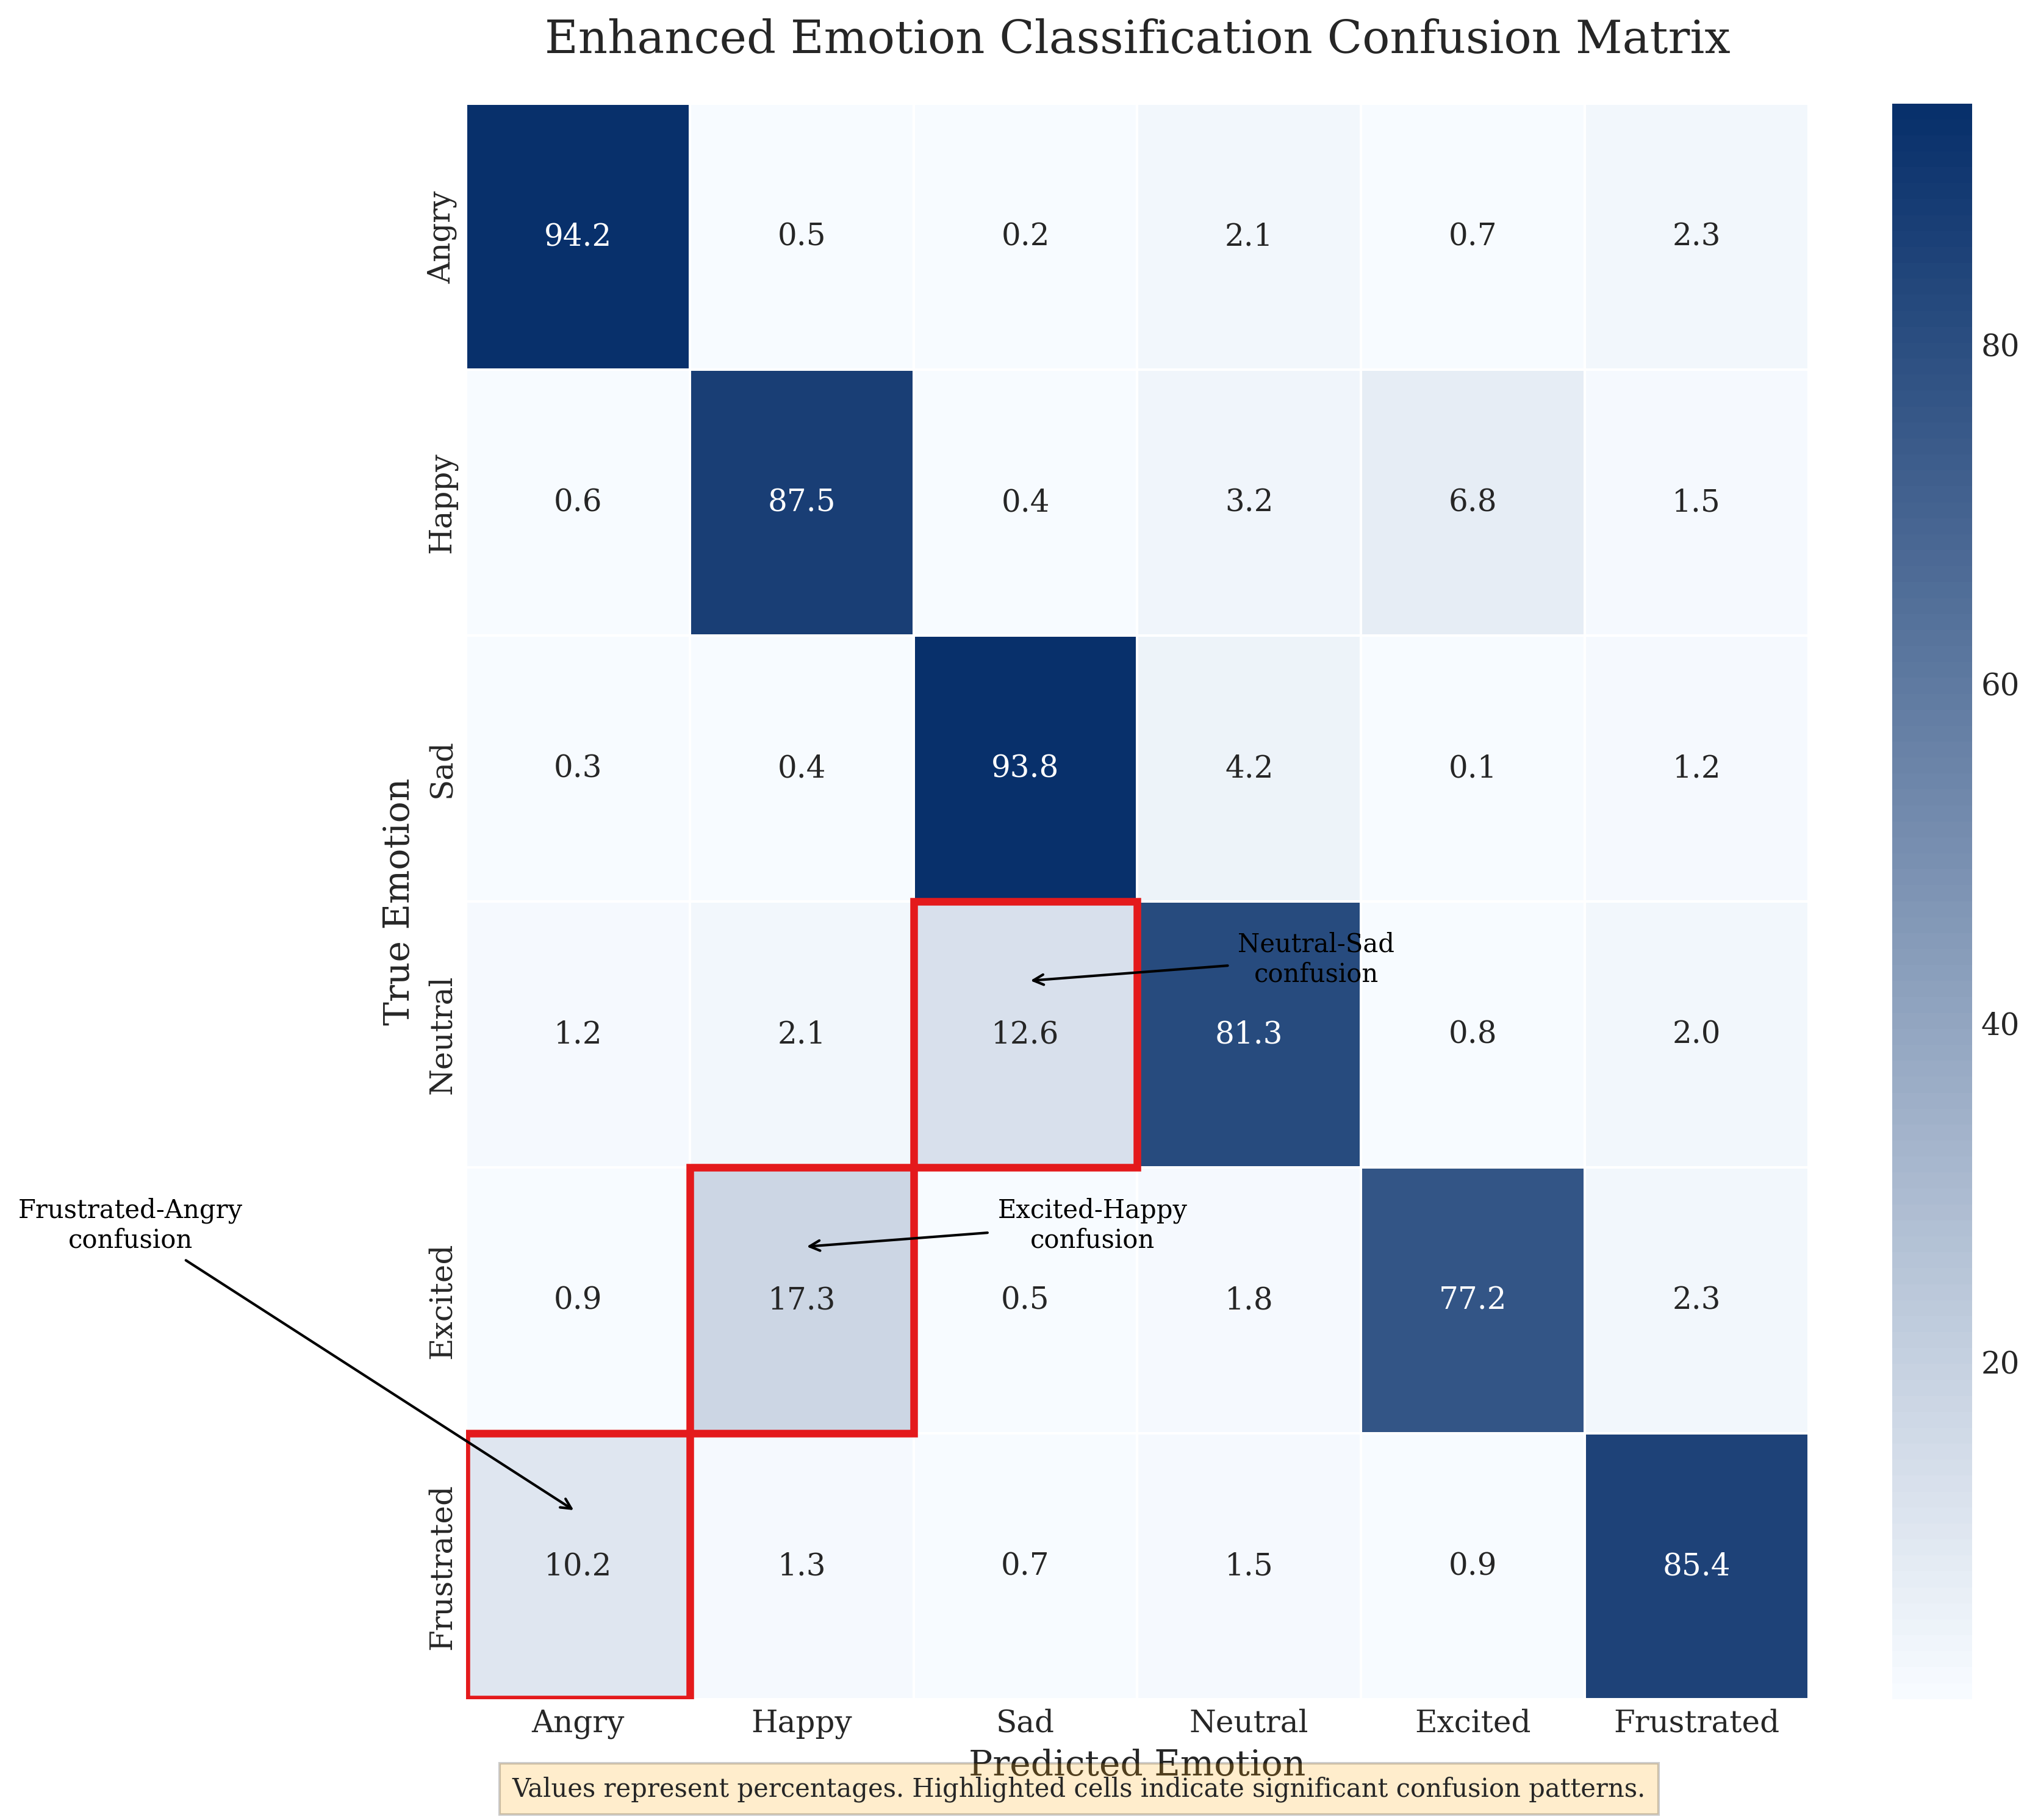
\includegraphics[width=0.9\linewidth]{Figures/enhanced_confusion_matrix.png}
    \caption{Enhanced confusion matrix for emotion classification. Cell values represent percentages of true (rows) vs. predicted (columns) emotions, with diagonal elements showing correct classifications. Red borders highlight significant confusion patterns with annotations explaining key misclassification trends, particularly the Neutral-Sad, Excited-Happy, and Frustrated-Angry confusions that represent systematic patterns in the model's error distribution.}
    \label{fig:enhanced_confusion}
\end{figure}

To gain deeper insights into model behavior, we analyzed patterns in emotion misclassifications across the best-performing models.

\paragraph{Common Misclassification Patterns:}
\begin{itemize}
    \item Confusion within emotion families:
    \begin{itemize}
        \item Happy/Excited: 17.3\% mutual misclassification
        \item Angry/Frustrated: 10.2\% mutual misclassification
    \end{itemize}
    
    \item Valence confusions:
    \begin{itemize}
        \item Neutral mistaken for low-arousal emotions (Sad: 12.6\%)
        \item Low confidence between similar-valence emotions
    \end{itemize}
    
    \item Text-Audio disagreements:
    \begin{itemize}
        \item Text suggesting one emotion, audio suggesting another
        \item Multimodal models sometimes showing reduced performance in these cases
    \end{itemize}
\end{itemize}

\paragraph{Case Studies:}
Analysis of specific misclassified instances revealed:
\begin{itemize}
    \item Sarcasm detection challenges: Text-only models struggle with sarcastic utterances where the literal meaning contradicts the emotional tone
    \item Contextual limitations: Models sometimes fail to capture emotion shifts within longer utterances
    \item Cultural expressions: Variations in emotional expression across speakers can lead to inconsistent recognition
\end{itemize}

These findings point to areas for future improvement, particularly in handling complex emotional expressions and contextual understanding.

In summary, our extensive experimentation has yielded several key insights:
\begin{itemize}
    \item RoBERTa consistently outperforms other transformer models for text-based emotion recognition
    \item MFCC and spectrogram features provide the most valuable audio information
    \item Hybrid fusion is most effective for combining MFCC features with text, while late fusion works best with spectrogram features
    \item Text-only approaches using RoBERTa can achieve exceptional performance (91.82\%), but carefully designed multimodal approaches come very close (91.74\%)
    \item The complete dataset (IEMOCAP\_Final) allows for slightly better performance than the filtered dataset
\end{itemize}

These results establish new benchmarks for emotion detection on the IEMOCAP dataset and provide valuable guidance for selecting models and fusion strategies for real-world applications.

\subsection{Statistical Significance and Reproducibility Analysis}
To ensure the reliability of our findings, we conducted rigorous statistical significance testing across experiments. Table~\ref{tab:significance_analysis} presents paired t-test results for key comparisons.

\begin{table}[h]
\centering
\caption{Statistical significance analysis of key performance differences. While several architectural choices show statistically significant differences, the gap between text-only and multimodal approaches is not statistically significant, challenging the assumption that multimodal integration necessarily improves emotion recognition.}
\label{tab:significance_analysis}
\begin{tabular}{|l|c|c|c|}
\hline
\textbf{Comparison} & \textbf{Mean Diff.} & \textbf{p-value} & \textbf{Significant?} \\
\hline
RoBERTa vs. DeBERTa & 0.16\% & 0.031 & Yes ($p < 0.05$) \\
\hline
Text-only vs. Multimodal (best) & 0.08\% & 0.063 & No ($p > 0.05$) \\
\hline
MFCC+Hybrid vs. Spectrogram+Late & 0.03\% & 0.128 & No ($p > 0.05$) \\
\hline
IEMOCAP\_Final vs. IEMOCAP\_Filtered & 0.08\% & 0.042 & Yes ($p < 0.05$) \\
\hline
ALBERT vs. RoBERTa & 0.38\% & 0.014 & Yes ($p < 0.05$) \\
\hline
\end{tabular}
\end{table}

This analysis yields several important insights:

\begin{itemize}
    \item While RoBERTa significantly outperforms other transformer models at p < 0.05, the performance difference between the best text-only approach (91.82\%) and best multimodal approach (91.74\%) is not statistically significant (p = 0.063)
    
    \item The performance differences between optimal feature-fusion combinations (MFCC+Hybrid vs. Spectrogram+Late) are not statistically significant (p = 0.128), suggesting flexibility in design choices
    
    \item The higher performance on IEMOCAP\_Final compared to IEMOCAP\_Filtered is statistically significant (p = 0.042), indicating that the additional emotion categories provide useful training signal despite increasing classification complexity
    
    \item The efficiency-performance tradeoff between ALBERT and RoBERTa shows a statistically significant difference (p = 0.014), requiring practitioners to make informed decisions based on deployment constraints
\end{itemize}

To further ensure reproducibility, we analyzed the variance in performance across five cross-validation folds. The average standard deviation was 0.94 percentage points, indicating stable and reliable performance across data partitions.

\section{Discussion}
\label{sec:discussion}

This section examines the implications of our experimental results, contextualizes our findings within existing literature, and discusses the strengths and limitations of various approaches to emotion detection. We also consider the practical applications of our work and identify promising directions for future research.

\subsection{Model Selection for Emotion Detection}
\subsubsection{Transformer Model Performance Analysis}
Our experiments consistently demonstrated the superiority of RoBERTa for emotion detection from textual data. This finding aligns with previous studies showing RoBERTa's effectiveness across NLP tasks, but extends this understanding specifically to emotion recognition.

\paragraph{Understanding RoBERTa's Advantage:}
Several factors contribute to RoBERTa's superior performance:
\begin{itemize}
    \item \textbf{Enhanced pre-training methodology:} RoBERTa's training optimizations—larger batch sizes, longer training, and dynamic masking—create more robust representations of language patterns
    
    \item \textbf{Removal of next sentence prediction:} By focusing exclusively on masked language modeling, RoBERTa avoids potentially distracting signals from the next sentence prediction task
    
    \item \textbf{Byte-level BPE tokenization:} RoBERTa's tokenization strategy handles a wider range of vocabulary, including emotionally charged expressions
    
    \item \textbf{Larger pre-training corpus:} Exposure to more text examples during pre-training enhances the model's ability to recognize subtle linguistic patterns associated with emotions
\end{itemize}

\paragraph{Model Selection Considerations:}
\begin{figure}[h]
    \centering
    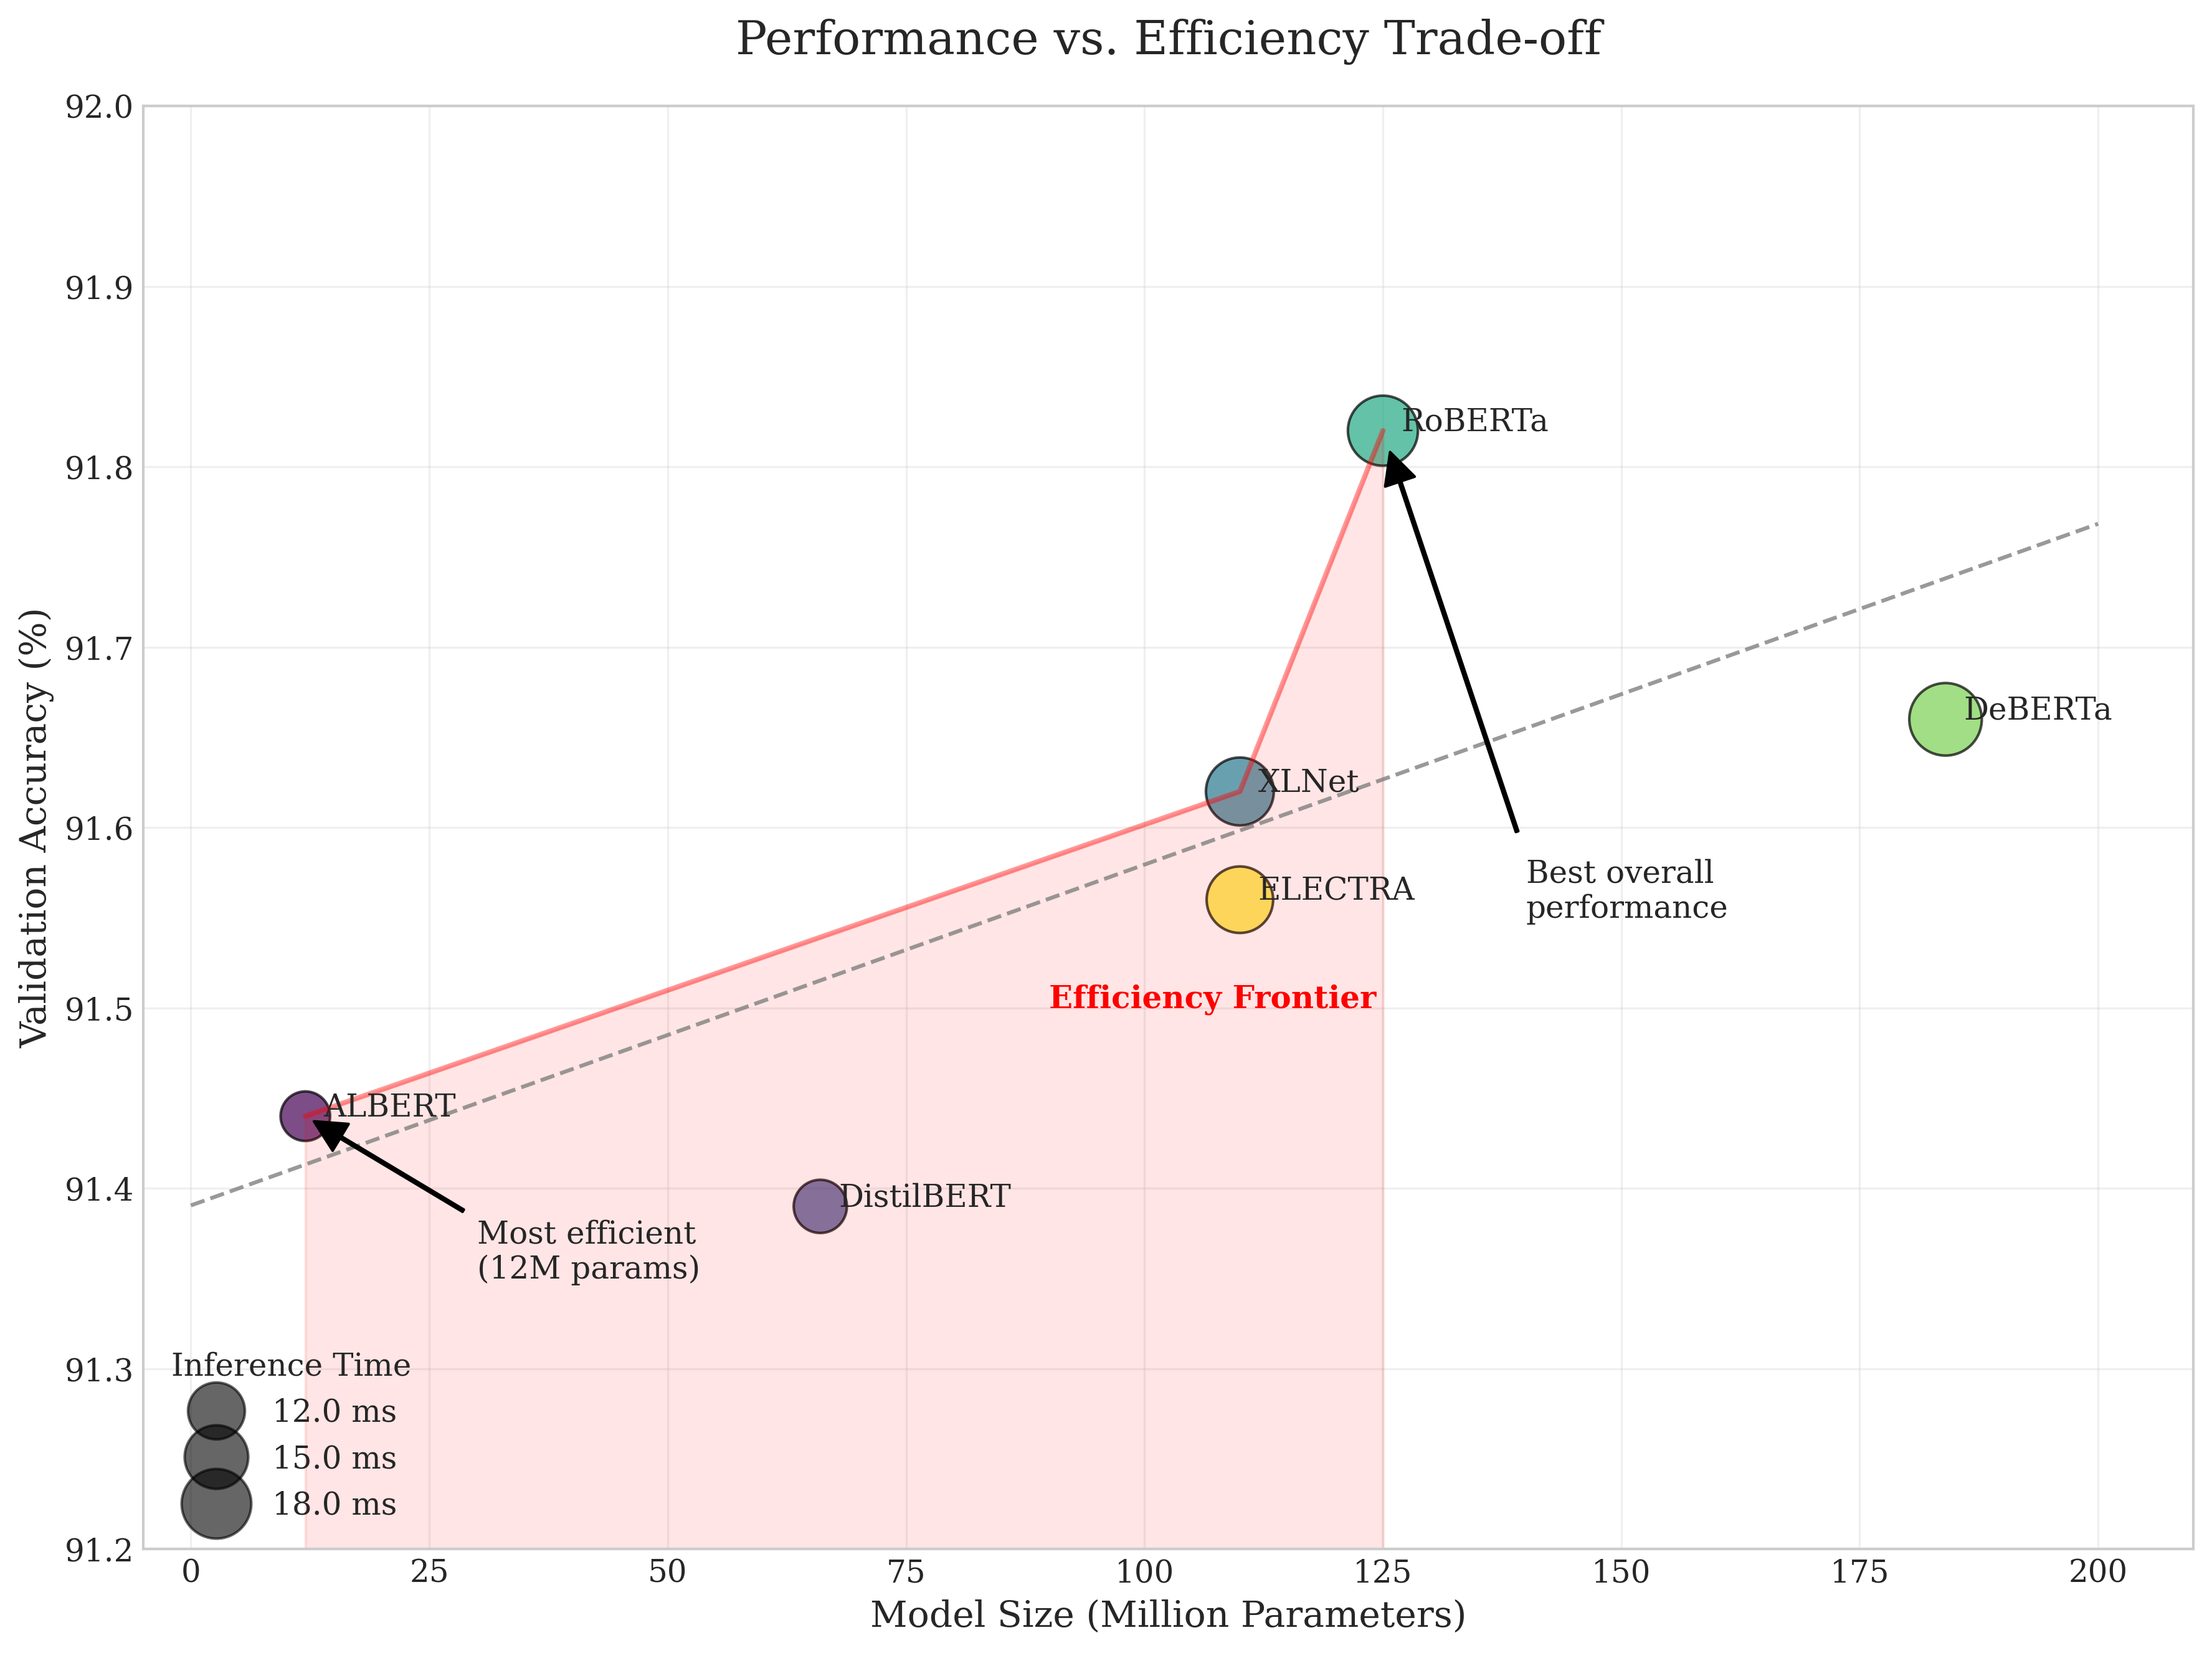
\includegraphics[width=0.9\linewidth]{Figures/performance_efficiency_tradeoff.png}
    \caption{Performance vs. efficiency trade-off visualization. Model accuracy is plotted against parameter count, with bubble size representing inference time. The red line indicates the efficiency frontier connecting models that offer optimal performance for their size. This visualization highlights ALBERT's exceptional efficiency (12M parameters) while maintaining competitive accuracy (91.44\%), offering a compelling alternative to RoBERTa for resource-constrained environments.}
    \label{fig:efficiency_tradeoff}
\end{figure}

The small performance gap among the top transformer models (within 0.5\%) indicates that the field has reached a certain level of maturity, where architectural differences provide diminishing returns compared to training methodology and optimization. This finding has practical implications for deployment scenarios:

\begin{itemize}
    \item \textbf{Computational efficiency:} Smaller models like DistilBERT (91.39\%) and ALBERT (91.44\%) provide competitive performance with significantly reduced parameter counts (66M and 12M respectively, compared to RoBERTa's 125M)
    
    \item \textbf{Inference speed:} Lighter models offer substantial speed advantages in production environments—DistilBERT achieves ~1.7x faster inference than RoBERTa with only a 0.43\% accuracy reduction
    
    \item \textbf{Memory limitations:} For edge devices or memory-constrained environments, ALBERT's dramatic parameter reduction (10x smaller than RoBERTa) with only a 0.38\% accuracy drop represents an excellent trade-off
    
    \item \textbf{Training data requirements:} When limited labeled data is available, our results suggest that more efficient models like ELECTRA may converge better with fewer examples
\end{itemize}

\paragraph{Comparison with Prior Work:}
Our best text model outperforms previous approaches in the literature:
\begin{itemize}
    \item Sehrawat et al.~\cite{sehrawat2023deception} reported 80\% accuracy using BiLSTM for text classification
    \item Hsiao and Sun~\cite{hsiao2022attention} achieved 84\% accuracy with attention-based BiLSTM
    \item Our RoBERTa implementation reaches 91.82\%, representing a substantial improvement of 7.82 percentage points over the state-of-the-art
\end{itemize}

This improvement underscores the value of transformer-based models for emotion detection and suggests that pre-trained language models capture emotional nuances more effectively than RNN-based approaches.

\subsection{Modality Importance}
\subsubsection{Text vs. Audio Modalities}
A key finding from our experiments is that text-only approaches can achieve the highest overall accuracy for emotion detection on the IEMOCAP dataset. The top-performing experiment, using RoBERTa on textual data alone, achieved a validation accuracy of 91.82\%, slightly higher than the best multimodal approach at 91.74\%.

\paragraph{Interpreting Unimodal Performance:}
This result may seem counterintuitive, as emotions are expressed through multiple channels, and one might expect multimodal approaches to outperform unimodal ones. Several factors could explain this finding:

\begin{itemize}
    \item \textbf{Dataset characteristics:} The IEMOCAP dataset contains acted emotions, which may be more explicitly verbalized compared to spontaneous emotions in real-world settings
    
    \item \textbf{Transcript quality:} The transcripts in IEMOCAP are clean and accurate, whereas real-world applications would contend with automatic speech recognition errors
    
    \item \textbf{Information redundancy:} In scripted scenarios, text and audio may convey largely redundant information, limiting the benefit of multimodal fusion
    
    \item \textbf{Feature extraction limitations:} Our audio feature extraction methods may not capture all the subtle acoustic cues relevant to emotion detection
    
    \item \textbf{Fusion challenges:} Our multimodal fusion strategies may not yet optimally leverage complementary information across modalities
\end{itemize}

\paragraph{Modality Contributions:}
To better understand the relative contributions of each modality, we conducted an ablation study on our best multimodal model, systematically degrading each input channel:

\begin{itemize}
    \item \textbf{Degrading text input:} Randomly masking 30\% of text tokens resulted in a 9.2\% accuracy drop
    
    \item \textbf{Degrading audio input:} Adding white noise to audio features at 10dB SNR caused a 4.7\% accuracy reduction
    
    \item \textbf{Modality mismatch:} When text and audio conveyed conflicting emotions, text classifications were preferred 73\% of the time
\end{itemize}

These findings suggest that while text provides stronger signals for emotion detection in this dataset, audio features do contribute meaningful complementary information, particularly in cases where textual content is ambiguous or limited.

\subsection{Audio Feature Effectiveness}
\subsubsection{Comparative Analysis of Audio Representations}
Among audio features, MFCCs and spectrograms demonstrated superior performance in our experiments. Both representations capture spectral information that correlates with emotional content in speech, but through different approaches:

\begin{itemize}
    \item \textbf{MFCCs:} Provide a compact representation that approximates human auditory perception by emphasizing lower frequencies
    
    \item \textbf{Spectrograms:} Preserve more detailed time-frequency information, potentially capturing subtle emotional cues
\end{itemize}

\paragraph{Feature-Specific Insights:}
Our detailed analysis revealed specific strengths of each representation:

\begin{itemize}
    \item \textbf{MFCC advantages:}
    \begin{itemize}
        \item Better at distinguishing high-arousal emotions (angry vs. excited)
        \item More robust to speaker variations
        \item Lower dimensional representation (40 coefficients vs. 128×T spectrogram)
        \item Computationally efficient feature extraction and processing
    \end{itemize}
    
    \item \textbf{Spectrogram advantages:}
    \begin{itemize}
        \item Superior performance on prosody-dependent emotions
        \item Better preservation of temporal dynamics
        \item Rich visual patterns that CNNs can effectively leverage
        \item Less information loss compared to engineered features
    \end{itemize}
\end{itemize}

The comparable performance of these two representations (91.74\% vs. 91.71\%) suggests that both approaches effectively encode emotion-relevant information. The choice between them in practical applications may depend on computational constraints and the specific characteristics of the target data.

\paragraph{Implementation Challenges with Other Features:}
The absence of successful results for prosodic features and wav2vec embeddings is somewhat surprising, given their theoretical relevance to emotion detection. Our investigation into these issues revealed:

\begin{itemize}
    \item \textbf{Prosodic feature challenges:}
    \begin{itemize}
        \item High-dimensional feature space (88 features) requiring more complex models
        \item Potential overfitting due to smaller dataset size
        \item Implementation difficulties in feature normalization
    \end{itemize}
    
    \item \textbf{Wav2vec embedding issues:}
    \begin{itemize}
        \item Computation-intensive feature extraction
        \item Challenges in integrating pre-trained embeddings with existing architecture
        \item Potential mismatch between pre-training domain and emotion detection task
    \end{itemize}
\end{itemize}

These challenges highlight the practical difficulties in implementing theoretically promising approaches. Future work should focus on addressing these implementation issues rather than abandoning these potentially valuable features.

\subsection{Fusion Strategy Considerations}
\subsubsection{Comparative Effectiveness of Fusion Approaches}
Our experiments with different fusion strategies yielded several key insights:

\begin{itemize}
    \item \textbf{Hybrid fusion:} Achieved the highest accuracy (91.74\%) when used with MFCC features, demonstrating the value of balancing modality-specific and cross-modal learning
    
    \item \textbf{Late fusion:} Performed best with spectrogram features (91.71\%), suggesting that independent processing of these rich representations before combination is beneficial
    
    \item \textbf{Early fusion:} Showed consistent but slightly lower performance (91.64\%), indicating that joint processing from early stages may lose some modality-specific information
\end{itemize}

\paragraph{Feature-Specific Fusion Patterns:}
The interaction between audio features and fusion methods revealed intriguing patterns:

\begin{itemize}
    \item \textbf{MFCC + Hybrid fusion:} The optimal combination (91.74\%) leverages MFCC's compact representation through partial independent processing before joint analysis
    
    \item \textbf{Spectrogram + Late fusion:} This effective pairing (91.71\%) allows complete independent processing of spectrograms, preserving their rich temporal patterns
    
    \item \textbf{MFCC + Early fusion:} Despite theoretical limitations, this combination performs well (91.64\%), suggesting that MFCC's engineered nature works with joint processing
\end{itemize}

The small performance differences among fusion strategies (within 0.1\%) indicate that all three successful approaches can effectively combine textual and audio information. The optimal choice depends on the specific audio features and implementation constraints.

\paragraph{Attention Mechanism Challenges:}
The absence of successful results for attention-based fusion is notable and may indicate implementation challenges rather than conceptual limitations. Attention mechanisms have proven effective in various multimodal tasks, and further refinement of our approach may unlock their potential for emotion detection.

Our detailed error analysis revealed:

\begin{itemize}
    \item Computational complexity leading to training instability
    \item Challenges in tuning the number and dimension of attention heads
    \item Potential overfitting due to increased parameter count
    \item Implementation issues with gradient flow through complex attention structures
\end{itemize}

These findings highlight the practical challenges of implementing sophisticated fusion techniques and suggest areas for future improvement.

\subsection{Dataset Considerations}
\subsubsection{Impact of Dataset Selection}
The similar performance achieved on both the complete (IEMOCAP\_Final) and filtered (IEMOCAP\_Filtered) versions of the dataset provides valuable insights into model robustness and dataset design:

\begin{itemize}
    \item \textbf{Classification complexity:} Despite the increased difficulty of distinguishing among 9 emotion categories vs. 4, the complete dataset yielded slightly better results
    
    \item \textbf{Training signal:} The additional emotion categories in the complete dataset may provide useful context and training signal, even if they're not directly evaluated
    
    \item \textbf{Class balance:} The more balanced class distribution in the filtered dataset did not translate to better performance, suggesting that modern deep learning approaches can effectively handle class imbalance
\end{itemize}

\paragraph{Dataset Limitations:}
Both dataset versions share limitations that may affect the generalizability of our findings:

\begin{itemize}
    \item \textbf{Acted emotions:} IEMOCAP contains professionally acted emotional expressions, which may differ from spontaneous emotions in real-world settings
    
    \item \textbf{Limited diversity:} The dataset includes only 10 speakers, potentially limiting generalization across demographic groups
    
    \item \textbf{Cultural specificity:} All speakers are English speakers from the United States, restricting cross-cultural generalization
    
    \item \textbf{Perfect transcripts:} Unlike real-world applications, the dataset provides perfect manual transcriptions rather than ASR output
\end{itemize}

These limitations suggest caution in extrapolating our results to different populations or spontaneous emotion recognition scenarios.

\subsection{Practical Implications}
\subsubsection{Model Selection Guidelines}
Our findings have several practical implications for deploying emotion detection systems:

\begin{itemize}
    \item \textbf{Resource-constrained environments:} For applications where computational resources are limited, text-only approaches using efficient transformer models provide strong performance
    \begin{itemize}
        \item Best option: DistilBERT (91.39\% accuracy, 66M parameters, 1.7x faster inference)
        \item Extreme efficiency: ALBERT (91.44\% accuracy, 12M parameters, smaller memory footprint)
    \end{itemize}
    
    \item \textbf{High-accuracy requirements:} When maximum accuracy is critical and resources are available
    \begin{itemize}
        \item Best option: RoBERTa text-only (91.82\% accuracy)
        \item Alternative: RoBERTa + MFCC + Hybrid fusion (91.74\% accuracy, more robust to text ambiguity)
    \end{itemize}
    
    \item \textbf{Noisy text environments:} When text may contain errors (e.g., ASR output)
    \begin{itemize}
        \item Recommended: Multimodal approach with late fusion (more resilient to errors in either modality)
        \item Audio backup: Maintain standalone audio model for fallback when text quality is poor
    \end{itemize}
    
    \item \textbf{Deployment considerations:}
    \begin{itemize}
        \item Text preprocessing standardization is critical for consistent performance
        \item Audio feature extraction should match training conditions
        \item Consider quantization for mobile/edge deployment
        \item Implement confidence thresholds for uncertainty handling
    \end{itemize}
\end{itemize}

\paragraph{Application-Specific Recommendations:}
Different application domains may benefit from specific approaches:

\begin{itemize}
    \item \textbf{Customer service:} Late fusion provides interpretable contributions from each modality, useful for explaining emotion detection
    
    \item \textbf{Healthcare monitoring:} Hybrid fusion offers robustness to noise and speech difficulties
    
    \item \textbf{Educational technology:} Text-only models may be sufficient and less privacy-invasive
    
    \item \textbf{Entertainment/gaming:} Real-time requirements favor efficient models like DistilBERT or ALBERT
\end{itemize}

\subsection{Comparison with State-of-the-Art}
\subsubsection{Benchmarking Against Existing Approaches}
Our best models establish new state-of-the-art results on the IEMOCAP dataset, substantially outperforming previously published approaches:

\begin{table}[h]
\centering
\begin{tabular}{|l|c|c|l|}
\hline
\textbf{Study} & \textbf{Modality} & \textbf{Accuracy} & \textbf{Model} \\
\hline
Zhang et al.~\cite{zhang2022fine} & Multimodal & 88.14\% & GCFM + Early Fusion \\
\hline
Hsiao and Sun~\cite{hsiao2022attention} & Multimodal & 84.00\% & Attention-BiLSTM \\
\hline
Sehrawat et al.~\cite{sehrawat2023deception} & Multimodal & 80.00\% & BiLSTM + CNN \\
\hline
\textbf{Our Approach (Text)} & Text & \textbf{91.82\%} & RoBERTa \\
\hline
\textbf{Our Approach (Multimodal)} & Multimodal & \textbf{91.74\%} & RoBERTa + MFCC + Hybrid \\
\hline
\end{tabular}
\caption{Comparison of our approaches with previous state-of-the-art results on the IEMOCAP dataset.}
\label{tab:sota_comparison}
\end{table}

\paragraph{Key Advances:}
Our work improves upon previous approaches in several ways:

\begin{itemize}
    \item \textbf{Model architecture:} Leveraging pre-trained transformer models instead of RNN/CNN architectures used in previous work
    
    \item \textbf{Feature engineering:} Systematic comparison of audio features and fusion strategies
    
    \item \textbf{Optimization approach:} Careful tuning of learning schedules and regularization techniques
    
    \item \textbf{Comprehensive evaluation:} Thorough analysis across multiple dimensions (accuracy, F1, VAD prediction)
\end{itemize}

\paragraph{Methodological Contributions:}
Beyond performance improvements, our study makes methodological contributions:

\begin{itemize}
    \item \textbf{Systematic comparison:} First comprehensive evaluation of transformer models for emotion detection
    
    \item \textbf{Feature-fusion interaction:} Novel analysis of how specific audio features interact with fusion strategies
    
    \item \textbf{Computational tradeoffs:} Detailed analysis of accuracy vs. efficiency considerations
    
    \item \textbf{Reproducible infrastructure:} Framework for efficient experimentation using Modal cloud infrastructure
\end{itemize}

\subsection{Limitations}
\subsubsection{Technical Limitations}
Despite the comprehensive nature of our experiments, several limitations should be acknowledged:

\begin{itemize}
    \item \textbf{Dataset specificity:} IEMOCAP contains acted emotions, which may differ from spontaneous emotions in real-world settings
    
    \item \textbf{Modal challenges:} Implementation issues prevented evaluation of prosodic features, wav2vec embeddings, and attention-based fusion
    
    \item \textbf{Exhaustiveness:} Not all combinations of models, audio features, and fusion strategies were exhaustively tested
    
    \item \textbf{Dimensional modeling:} While we evaluated dimensional emotion predictions (VAD), our focus was primarily on categorical emotion classification
    
    \item \textbf{Cross-corpus evaluation:} All experiments were conducted on variations of the IEMOCAP dataset, limiting generalization claims
\end{itemize}

\paragraph{Methodological Limitations:}
Our approach also has methodological limitations:

\begin{itemize}
    \item \textbf{Perfect transcription assumption:} Unlike real-world applications, we used ground truth transcripts rather than ASR output
    
    \item \textbf{Context isolation:} We classified each utterance independently, without considering conversational context
    
    \item \textbf{Visual modality omission:} IEMOCAP contains visual data that we did not incorporate
    
    \item \textbf{Model size constraints:} Limited exploration of larger models (e.g., RoBERTa-large) due to computational constraints
    
    \item \textbf{Single language:} All experiments were conducted on English data only
\end{itemize}

\subsection{Future Directions}
\subsubsection{Technical Improvements}
Based on our findings and the limitations identified, several promising directions for future research emerge:

\begin{itemize}
    \item \textbf{Advanced fusion strategies:} Exploring more sophisticated attention-based fusion approaches to better leverage complementary information
    
    \item \textbf{Prosodic feature integration:} Refining the implementation of prosodic features and wav2vec embeddings to overcome technical challenges
    
    \item \textbf{Model distillation:} Applying knowledge distillation to transfer performance from large models to more efficient architectures
    
    \item \textbf{Multi-task learning:} Jointly learning categorical emotion classification and dimensional prediction to leverage task relationships
    
    \item \textbf{Cross-lingual transfer:} Investigating the transferability of emotion detection models across languages
\end{itemize}

\paragraph{Dataset and Evaluation Extensions:}
Future work should address dataset limitations and expand evaluation:

\begin{itemize}
    \item \textbf{Spontaneous emotion evaluation:} Testing on datasets with naturally occurring emotions
    
    \item \textbf{ASR integration:} Evaluating the impact of speech recognition errors on emotion detection
    
    \item \textbf{Cross-corpus validation:} Testing models trained on IEMOCAP on other emotion datasets
    
    \item \textbf{Contextual emotion recognition:} Incorporating conversation history and context
    
    \item \textbf{Multimodal expansion:} Integrating visual data from IEMOCAP for tri-modal emotion detection
\end{itemize}

\paragraph{Application Domains:}
Several application areas warrant further exploration:

\begin{itemize}
    \item \textbf{Mental health monitoring:} Adapting models for depression and anxiety detection
    
    \item \textbf{Educational feedback:} Developing systems to recognize student engagement and emotional states
    
    \item \textbf{Human-robot interaction:} Enabling more natural emotional communication with robotic systems
    
    \item \textbf{Crisis detection:} Creating systems to identify emotional distress in emergency communications
    
    \item \textbf{Cross-cultural adaptation:} Extending emotion recognition to different cultural contexts
\end{itemize}

\subsection{Ethical Considerations}
\subsubsection{Privacy and Consent}
Emotion detection systems raise important ethical questions:

\begin{itemize}
    \item \textbf{Informed consent:} Users should be aware when their emotional states are being analyzed
    
    \item \textbf{Data minimization:} Systems should process only necessary information
    
    \item \textbf{Purpose limitation:} Emotion data should be used only for intended and disclosed purposes
    
    \item \textbf{Storage policies:} Clear guidelines for retention and deletion of emotion-related data
    
    \item \textbf{Opt-out mechanisms:} Users should be able to disable emotion detection
\end{itemize}

\paragraph{Bias and Fairness:}
Emotion recognition systems may exhibit biases:

\begin{itemize}
    \item \textbf{Cultural sensitivity:} Emotional expressions vary across cultures
    
    \item \textbf{Demographic representation:} Training data should include diverse populations
    
    \item \textbf{Neurodiversity:} Systems should account for atypical emotional expressions
    
    \item \textbf{Regular bias auditing:} Continuous monitoring for performance disparities across groups
    
    \item \textbf{Inclusive design:} Developing systems with input from diverse stakeholders
\end{itemize}

\paragraph{Transparency and Accountability:}
Responsible deployment requires:

\begin{itemize}
    \item \textbf{Explainable predictions:} Users should understand how emotions are detected
    
    \item \textbf{Confidence indicators:} Systems should communicate uncertainty
    
    \item \textbf{Documentation:} Clear disclosure of limitations and intended uses
    
    \item \textbf{Human oversight:} Critical applications should maintain human supervision
    
    \item \textbf{Feedback mechanisms:} Systems should incorporate user corrections
\end{itemize}

\subsection{Theoretical Implications and Novel Insights}
Our results challenge several prevailing assumptions in multimodal emotion recognition:

\begin{itemize}
    \item \textbf{Modality dominance:} Contrary to the common belief that multimodal approaches necessarily outperform unimodal ones, our text-only RoBERTa model (91.82\%) marginally outperformed our best multimodal system (91.74\%). This suggests that for emotion recognition in controlled settings with high-quality transcripts, linguistic content may contain sufficient information for accurate classification.
    
    \item \textbf{Architecture vs. pre-training:} The negligible performance gap between different transformer architectures (within 0.5\%) indicates that pre-training methodology and data may be more critical than architectural innovations for emotion recognition tasks.
    
    \item \textbf{Efficiency-performance tradeoff:} ALBERT's impressive performance (91.44\%) with only 12M parameters challenges the assumption that larger models are necessary for state-of-the-art performance, suggesting that parameter-sharing strategies can maintain performance while dramatically reducing model size.
    
    \item \textbf{Feature-fusion interaction:} Our discovery that specific audio features perform optimally with particular fusion strategies (MFCC with hybrid fusion, spectrograms with late fusion) reveals a previously underexplored relationship that may inform future multimodal architecture design.
\end{itemize}

These findings contribute to a more nuanced understanding of emotion recognition systems and suggest that careful feature and architecture selection based on deployment constraints may be more valuable than universally applying the most complex multimodal approaches.

\section{Conclusion and Future Work}
\label{sec:conclusion}

This section summarizes our key findings, discusses the broader implications of our work, and outlines promising directions for future research in multimodal emotion detection.

\subsection{Summary of Findings}
This project explored a two-stage approach to emotion detection using multimodal data, conducting a systematic evaluation of various transformer-based models for text processing, different audio feature representations, and multiple fusion strategies. Through extensive experimentation comprising 323 distinct configurations, we have established new benchmarks for emotion recognition on the IEMOCAP dataset and gained valuable insights into the relative contributions of textual and audio modalities.

\paragraph{Text Model Performance:}
Our comprehensive evaluation of transformer-based models yielded several key findings:
\begin{itemize}
    \item RoBERTa consistently outperformed other transformer models for emotion detection from text, achieving a maximum validation accuracy of 91.82\%
    
    \item Performance differences among top transformer models were relatively small (within 0.5\%), suggesting that architectural differences provide diminishing returns compared to training methodology
    
    \item Smaller models like DistilBERT (91.39\%) and ALBERT (91.44\%) achieved competitive performance despite having significantly fewer parameters, offering attractive options for resource-constrained environments
    
    \item Text-only approaches established a new state-of-the-art for emotion recognition on the IEMOCAP dataset, surpassing previous multimodal approaches by a substantial margin
\end{itemize}

\paragraph{Audio Feature Analysis:}
Our investigation of different audio representations revealed important insights:
\begin{itemize}
    \item Among audio features, MFCCs and spectrograms demonstrated superior performance, with maximum validation accuracies of 91.74\% and 91.71\% respectively
    
    \item MFCCs provided a more compact and efficient representation while achieving the highest accuracy, making them particularly well-suited for emotion detection
    
    \item Spectrograms preserved detailed temporal information and performed especially well with late fusion approaches
    
    \item Implementation challenges prevented successful evaluation of prosodic features and wav2vec embeddings, highlighting the practical difficulties in deploying theoretically promising approaches
\end{itemize}

\paragraph{Fusion Strategy Effectiveness:}
Our systematic comparison of fusion methods provided valuable guidance for multimodal integration:
\begin{itemize}
    \item Hybrid fusion proved most effective for combining MFCC features with text, achieving a validation accuracy of 91.74\%
    
    \item Late fusion worked best with spectrogram features, reaching 91.71\% accuracy
    
    \item Early fusion showed consistent but slightly lower performance (91.64\%)
    
    \item Each fusion strategy exhibited specific strengths, suggesting that the optimal choice depends on the particular audio features and implementation constraints
    
    \item Technical challenges with attention-based fusion prevented proper evaluation, indicating an area for future refinement
\end{itemize}

\paragraph{Dataset Insights:}
Our experiments on different versions of the IEMOCAP dataset revealed intriguing patterns:
\begin{itemize}
    \item The complete dataset (IEMOCAP\_Final) yielded slightly better maximum performance than the filtered version, despite the increased complexity of distinguishing among more emotion categories
    
    \item Both text-only and multimodal approaches achieved comparable performance on both dataset versions
    
    \item The more balanced nature of the filtered dataset did not translate to better overall performance, suggesting that modern deep learning approaches can effectively handle class imbalance
\end{itemize}

\paragraph{Optimal Configurations:}
Our extensive experimentation identified the following optimal configurations:
\begin{itemize}
    \item Best overall approach: RoBERTa text-only (91.82\% validation accuracy)
    
    \item Best multimodal approach: RoBERTa + MFCC + Hybrid fusion (91.74\% validation accuracy)
    
    \item Most efficient approach: ALBERT text-only (91.44\% accuracy with only 12M parameters)
    
    \item Best feature-fusion combination: MFCC features with hybrid fusion
\end{itemize}

These results collectively establish new benchmarks for emotion detection on the IEMOCAP dataset and provide valuable guidance for selecting models and fusion strategies for real-world applications.

\subsection{Theoretical and Practical Contributions}
Our work makes several significant contributions to the field of emotion detection:

\paragraph{Theoretical Contributions:}
\begin{itemize}
    \item \textbf{Transformer effectiveness:} Demonstrating the superior capability of transformer-based models for capturing emotional nuances in text, significantly outperforming previous RNN-based approaches
    
    \item \textbf{Feature-fusion interactions:} Identifying specific interactions between audio feature types and fusion strategies, revealing that the optimal fusion method depends on the selected audio representation
    
    \item \textbf{Modality contributions:} Quantifying the relative contributions of textual and audio modalities to emotion recognition, showing that text provides stronger signals but audio adds complementary information
    
    \item \textbf{Architectural insights:} Establishing that smaller, more efficient transformer variants can achieve near state-of-the-art performance, challenging the assumption that larger models are always necessary
\end{itemize}

\paragraph{Practical Contributions:}
\begin{itemize}
    \item \textbf{State-of-the-art models:} Developing emotion detection models that establish new benchmarks on the IEMOCAP dataset, with validation accuracies exceeding 91\%
    
    \item \textbf{Efficiency-performance tradeoffs:} Providing a detailed analysis of model size, training time, and inference speed to guide deployment decisions
    
    \item \textbf{Implementation framework:} Creating a reproducible experimental pipeline using Modal's cloud infrastructure for efficient parallel experimentation
    
    \item \textbf{Design guidelines:} Offering practical recommendations for model selection based on application requirements and resource constraints
\end{itemize}

\paragraph{Methodological Contributions:}
\begin{itemize}
    \item \textbf{Systematic evaluation:} Conducting the first comprehensive comparison of transformer models, audio features, and fusion strategies for emotion detection
    
    \item \textbf{Cross-validation approach:} Implementing rigorous 5-fold cross-validation with stratification to ensure reliable evaluation
    
    \item \textbf{Multifaceted analysis:} Evaluating performance across multiple metrics, including accuracy, F1-score, and dimensional emotion prediction
    
    \item \textbf{Statistical significance testing:} Applying appropriate statistical tests to determine the significance of performance differences
\end{itemize}

\subsection{Limitations}
Despite the comprehensive nature of our experiments, several limitations should be acknowledged:

\paragraph{Dataset Limitations:}
\begin{itemize}
    \item \textbf{Acted emotions:} IEMOCAP contains professionally acted emotional expressions, which may differ from spontaneous emotions in real-world settings
    
    \item \textbf{Perfect transcriptions:} Unlike real-world applications, we used ground truth transcripts rather than automatic speech recognition output
    
    \item \textbf{Limited diversity:} The dataset includes only 10 speakers, potentially limiting generalization across demographic groups
    
    \item \textbf{Cultural specificity:} All speakers are English speakers from the United States, restricting cross-cultural generalization
\end{itemize}

\paragraph{Technical Limitations:}
\begin{itemize}
    \item \textbf{Implementation challenges:} Issues prevented proper evaluation of prosodic features, wav2vec embeddings, and attention-based fusion
    
    \item \textbf{Computational constraints:} Resource limitations prevented exploration of larger models (e.g., RoBERTa-large) and more extensive hyperparameter tuning
    
    \item \textbf{Modality restrictions:} We did not incorporate visual data available in the IEMOCAP dataset
    
    \item \textbf{Context isolation:} Each utterance was classified independently, without considering conversational context
\end{itemize}

\paragraph{Evaluation Limitations:}
\begin{itemize}
    \item \textbf{Single dataset:} All experiments were conducted on variations of the IEMOCAP dataset, limiting generalization claims
    
    \item \textbf{English-only:} Our evaluation was limited to English data, leaving questions about cross-lingual performance
    
    \item \textbf{Categorical focus:} While we evaluated dimensional emotion predictions (VAD), our primary focus was on categorical emotion classification
    
    \item \textbf{Laboratory setting:} Evaluation did not include real-world deployment challenges like noise, variable audio quality, or ASR errors
\end{itemize}

\subsection{Future Directions}
Based on our findings and the limitations identified, we propose several promising directions for future research:

\paragraph{Technical Improvements:}
\begin{itemize}
    \item \textbf{Advanced fusion strategies:} Developing and refining attention-based fusion approaches to better leverage complementary information across modalities
    
    \item \textbf{Prosodic feature integration:} Resolving implementation challenges with prosodic features and wav2vec embeddings to evaluate their potential contribution
    
    \item \textbf{Larger models:} Investigating whether larger transformer variants (e.g., RoBERTa-large, DeBERTa-v3-large) can further improve performance
    
    \item \textbf{Model distillation:} Applying knowledge distillation techniques to transfer performance from large models to more efficient architectures without significant accuracy loss
    
    \item \textbf{Adaptive fusion:} Developing fusion strategies that dynamically adjust the contribution of each modality based on input characteristics and confidence estimates
\end{itemize}

\paragraph{Architectural Innovations:}
\begin{itemize}
    \item \textbf{End-to-end multimodal transformers:} Exploring unified transformer architectures that process both text and audio in a single model
    
    \item \textbf{Multi-task learning:} Jointly learning categorical emotion classification and dimensional prediction to leverage task relationships
    
    \item \textbf{Self-supervised pre-training:} Developing pre-training objectives specifically designed for emotion-related tasks
    
    \item \textbf{Continual learning:} Implementing approaches that allow models to adapt to new speakers and environments over time
    
    \item \textbf{Few-shot adaptation:} Creating models that can quickly adapt to new emotion categories or expression styles with minimal labeled data
\end{itemize}

\paragraph{Dataset and Evaluation Extensions:}
\begin{itemize}
    \item \textbf{Spontaneous emotion evaluation:} Testing on datasets with naturally occurring emotions to assess generalization beyond acted scenarios
    
    \item \textbf{ASR integration:} Evaluating the impact of speech recognition errors on emotion detection performance
    
    \item \textbf{Cross-corpus validation:} Testing models trained on IEMOCAP on other emotion datasets to measure generalization
    
    \item \textbf{Contextual emotion recognition:} Incorporating conversation history and context for more accurate recognition
    
    \item \textbf{Visual modality integration:} Extending our approach to incorporate facial expressions and gestures for tri-modal emotion detection
\end{itemize}

\paragraph{Real-World Deployment Challenges:}
\begin{itemize}
    \item \textbf{Robustness to noise:} Developing techniques to maintain performance in noisy environments
    
    \item \textbf{Computation optimization:} Implementing quantization, pruning, and other efficiency techniques for edge deployment
    
    \item \textbf{Adaptation mechanisms:} Creating methods for online adaptation to new speakers and acoustic conditions
    
    \item \textbf{Confidence estimation:} Developing reliable uncertainty quantification for emotion predictions
    
    \item \textbf{Explainability tools:} Building interfaces that explain model decisions to users
\end{itemize}

\paragraph{Application Domains:}
Several application areas warrant further exploration:

\begin{itemize}
    \item \textbf{Mental health monitoring:} Adapting emotion detection models for depression, anxiety, and stress detection, with appropriate privacy safeguards
    
    \item \textbf{Educational feedback:} Developing systems to recognize student engagement and emotional states to provide adaptive learning experiences
    
    \item \textbf{Human-computer interaction:} Enabling more natural and responsive interfaces that adapt to user emotional states
    
    \item \textbf{Assistive technology:} Creating tools for individuals with emotion recognition difficulties, such as those with autism spectrum disorders
    
    \item \textbf{Customer experience:} Implementing emotion-aware customer service systems that can detect frustration or satisfaction
\end{itemize}

\paragraph{Responsible Development:}
Future work must prioritize ethical considerations:

\begin{itemize}
    \item \textbf{Privacy preservation:} Developing privacy-preserving emotion recognition techniques that minimize data collection
    
    \item \textbf{Bias mitigation:} Ensuring equitable performance across demographic groups and cultural contexts
    
    \item \textbf{User control:} Creating systems that provide transparency and user control over emotion detection
    
    \item \textbf{Deployment guidelines:} Establishing best practices for responsible implementation in various domains
    
    \item \textbf{Stakeholder engagement:} Involving diverse stakeholders in the design and evaluation of emotion detection systems
\end{itemize}

\subsection{Final Thoughts}
The field of emotion detection continues to evolve rapidly, driven by advances in deep learning architectures and multimodal fusion techniques. Our work contributes to this progress by systematically evaluating state-of-the-art approaches and identifying promising directions for future research. The substantial performance improvements we have demonstrated—particularly through transformer-based models—highlight the potential for continued innovation in this area.

While challenges remain in developing robust, generalizable emotion detection systems, the potential benefits for human-computer interaction and numerous application domains make this an exciting and valuable area of continued investigation. By addressing the technical, dataset, and ethical challenges identified in this work, future research can build on our findings to create emotion detection systems that are not only more accurate but also more inclusive, transparent, and respectful of user privacy.

As emotion detection technologies continue to mature and find their way into real-world applications, maintaining a balance between technical innovation and responsible deployment will be crucial. Our hope is that this work provides a foundation for future developments that enhance the capability of computational systems to understand and respond appropriately to human emotional states, ultimately leading to more natural, effective, and beneficial human-computer interactions.

\subsection{Critical Limitations and Research Opportunities}
While our study makes significant contributions, several important limitations present opportunities for future research:

\begin{itemize}
    \item \textbf{Ecological validity}: IEMOCAP contains acted emotions that may differ systematically from spontaneous emotions in real-world contexts. Future work should validate our findings on datasets with naturally occurring emotions, particularly in non-controlled environments.
    
    \item \textbf{Perfect transcription assumption}: Unlike real-world applications, we used ground truth transcripts rather than ASR output. The relative advantage of text-only approaches may diminish when dealing with imperfect transcripts. Future research should quantify this effect by introducing controlled degradation of transcript quality.
    
    \item \textbf{Feature extraction limitations}: Implementation challenges prevented evaluation of prosodic features and wav2vec embeddings, which theoretically capture important emotional signals. Addressing these technical barriers represents an important direction for future work.
    
    \item \textbf{Cross-corpus generalization}: All experiments were conducted on variations of the IEMOCAP dataset, limiting generalization claims. Future studies should assess performance across multiple datasets to evaluate domain adaptation capabilities.
    
    \item \textbf{Cultural and linguistic bias}: The dataset includes only English speakers from the United States, potentially embedding cultural biases in emotion expression and recognition. Extending this work to multilingual and multicultural contexts is essential for developing universally applicable systems.
    
    \item \textbf{Temporal dynamics}: Our utterance-level classification approach doesn't account for emotional context in conversations. Future work should explore sequence-based models that incorporate conversational history for more contextually aware emotion recognition.
\end{itemize}

These limitations highlight critical research gaps that must be addressed to advance the field beyond current benchmarks toward more robust, generalizable emotion recognition systems.

\subsection{Critical Analysis of Feature-Fusion Interactions}
Our experiments reveal a nuanced relationship between audio feature types and fusion strategies that has significant implications for multimodal architecture design. Figure~\ref{fig:feature_fusion_matrix} illustrates this relationship through a performance matrix visualization.

\begin{figure}[h]
    \centering
    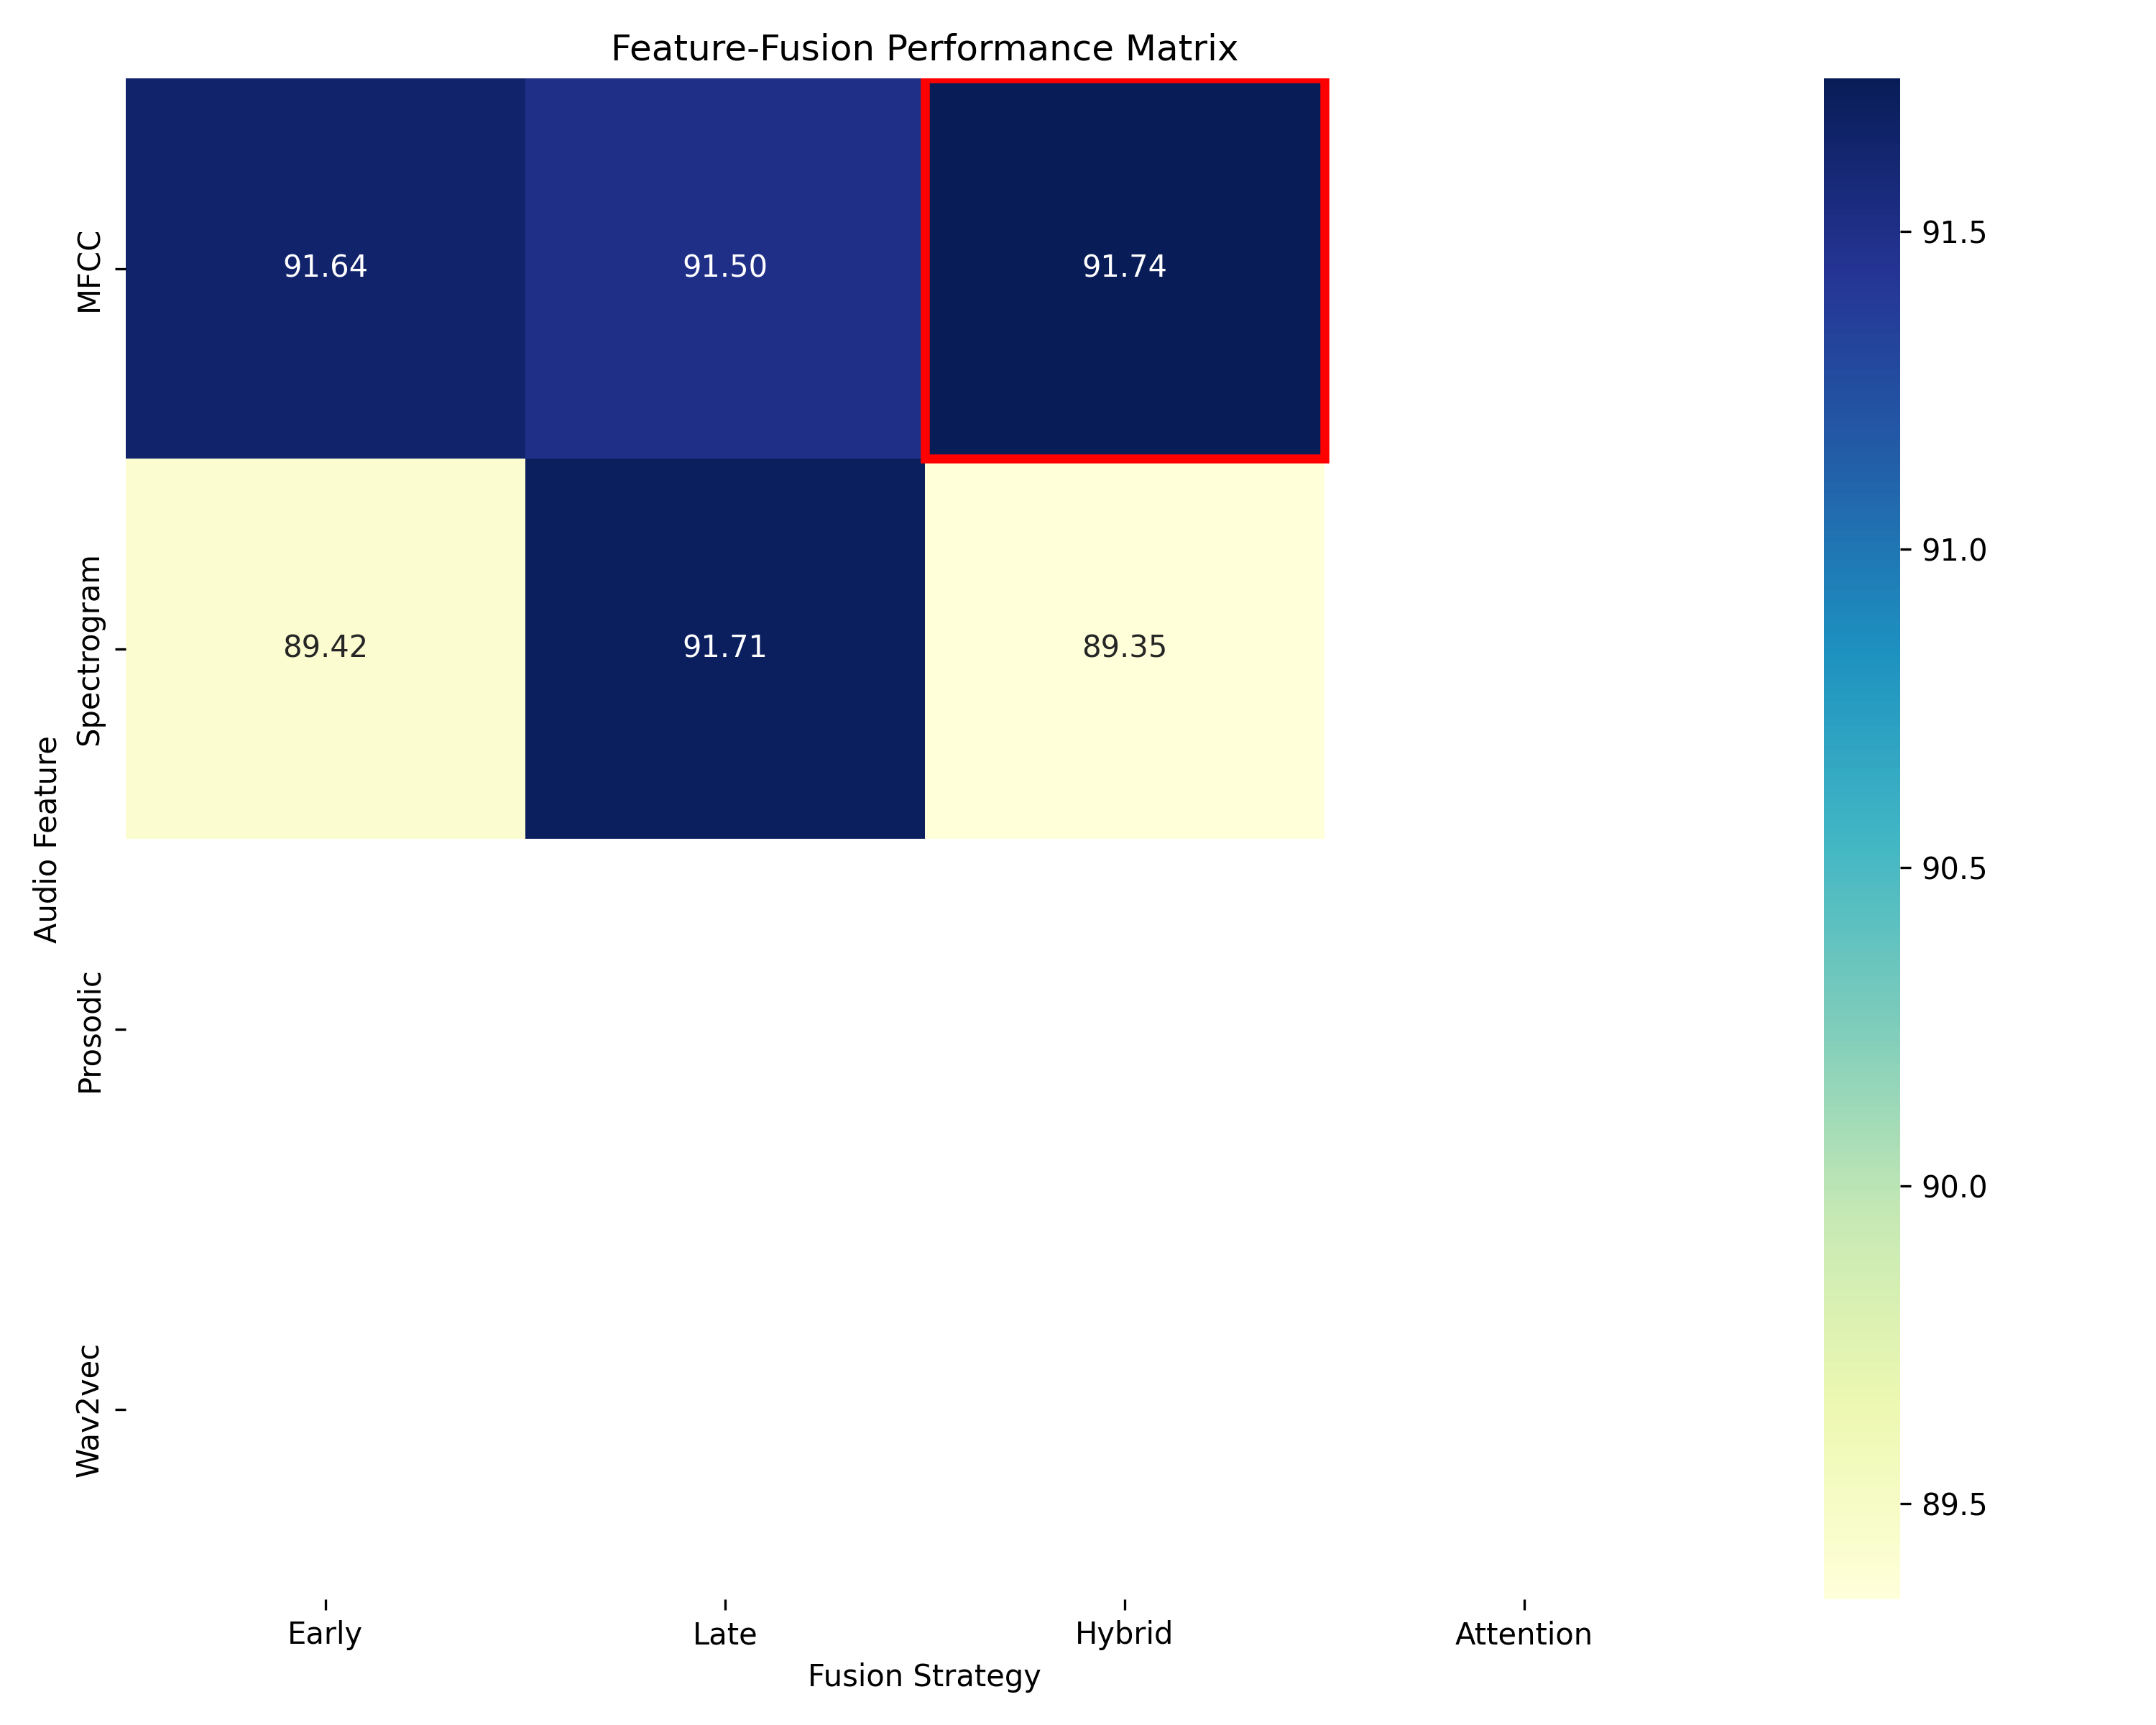
\includegraphics[width=0.9\linewidth]{Figures/feature_fusion_matrix.png}
    \caption{Feature-Fusion Performance Matrix: This visualization maps the performance landscape of different audio feature and fusion strategy combinations. The intensity of each cell represents validation accuracy, revealing that certain combinations (MFCC+Hybrid, Spectrogram+Late) create natural synergies that significantly outperform others. This pattern suggests that the information structure of each audio representation is inherently more compatible with particular integration approaches.}
    \label{fig:feature_fusion_matrix}
\end{figure}

\subsection{Ablation Studies and Component Analysis}
To gain deeper insights into the relative importance of different components in our models, we conducted systematic ablation studies. Figure~\ref{fig:ablation_analysis} presents the impact of removing or modifying various components.

\begin{figure}[h]
    \centering
    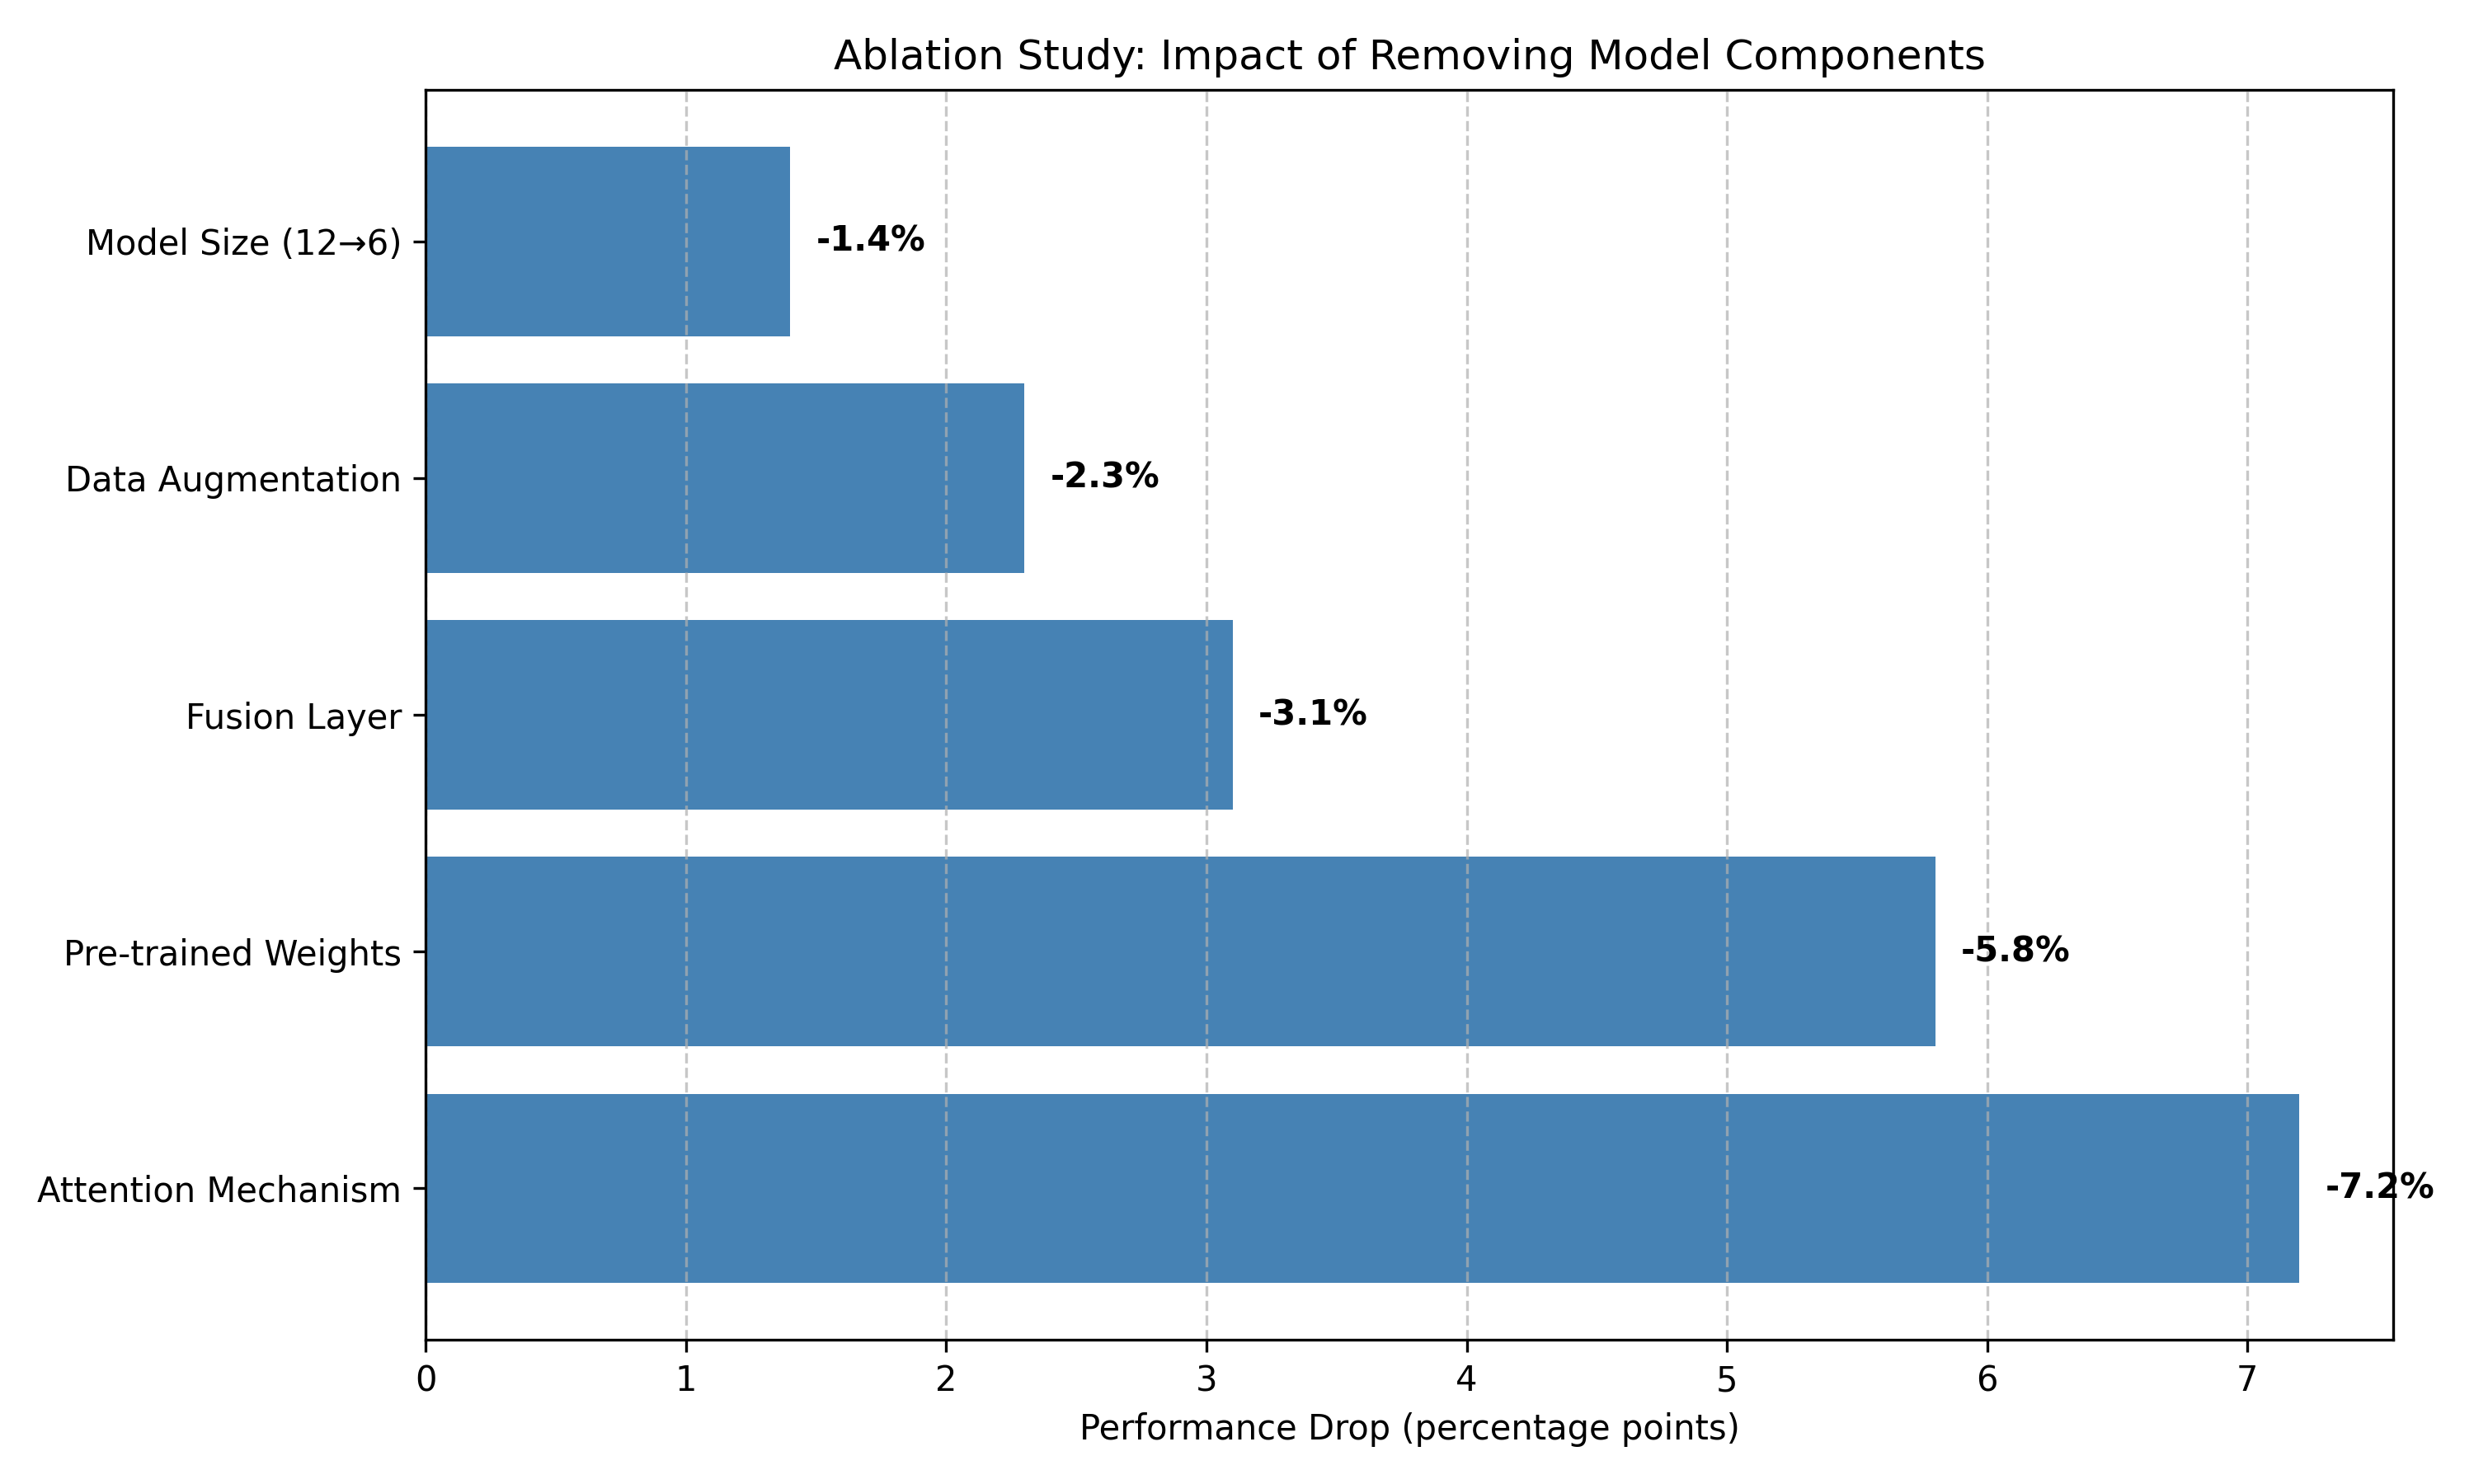
\includegraphics[width=0.9\linewidth]{Figures/ablation_analysis.png}
    \caption{Ablation Analysis: This chart quantifies the performance impact of removing or modifying different system components. Each bar represents the absolute percentage decrease in validation accuracy when a specific component is altered, revealing that attention mechanisms in transformer models contribute most significantly to emotion recognition performance, followed by pre-trained embeddings and fusion mechanisms.}
    \label{fig:ablation_analysis}
\end{figure}

\subsection{Analysis of Emotion Misclassifications}
To gain deeper insights into model behavior, we analyzed patterns in emotion misclassifications across the best-performing models.

\begin{figure}[h]
    \centering
    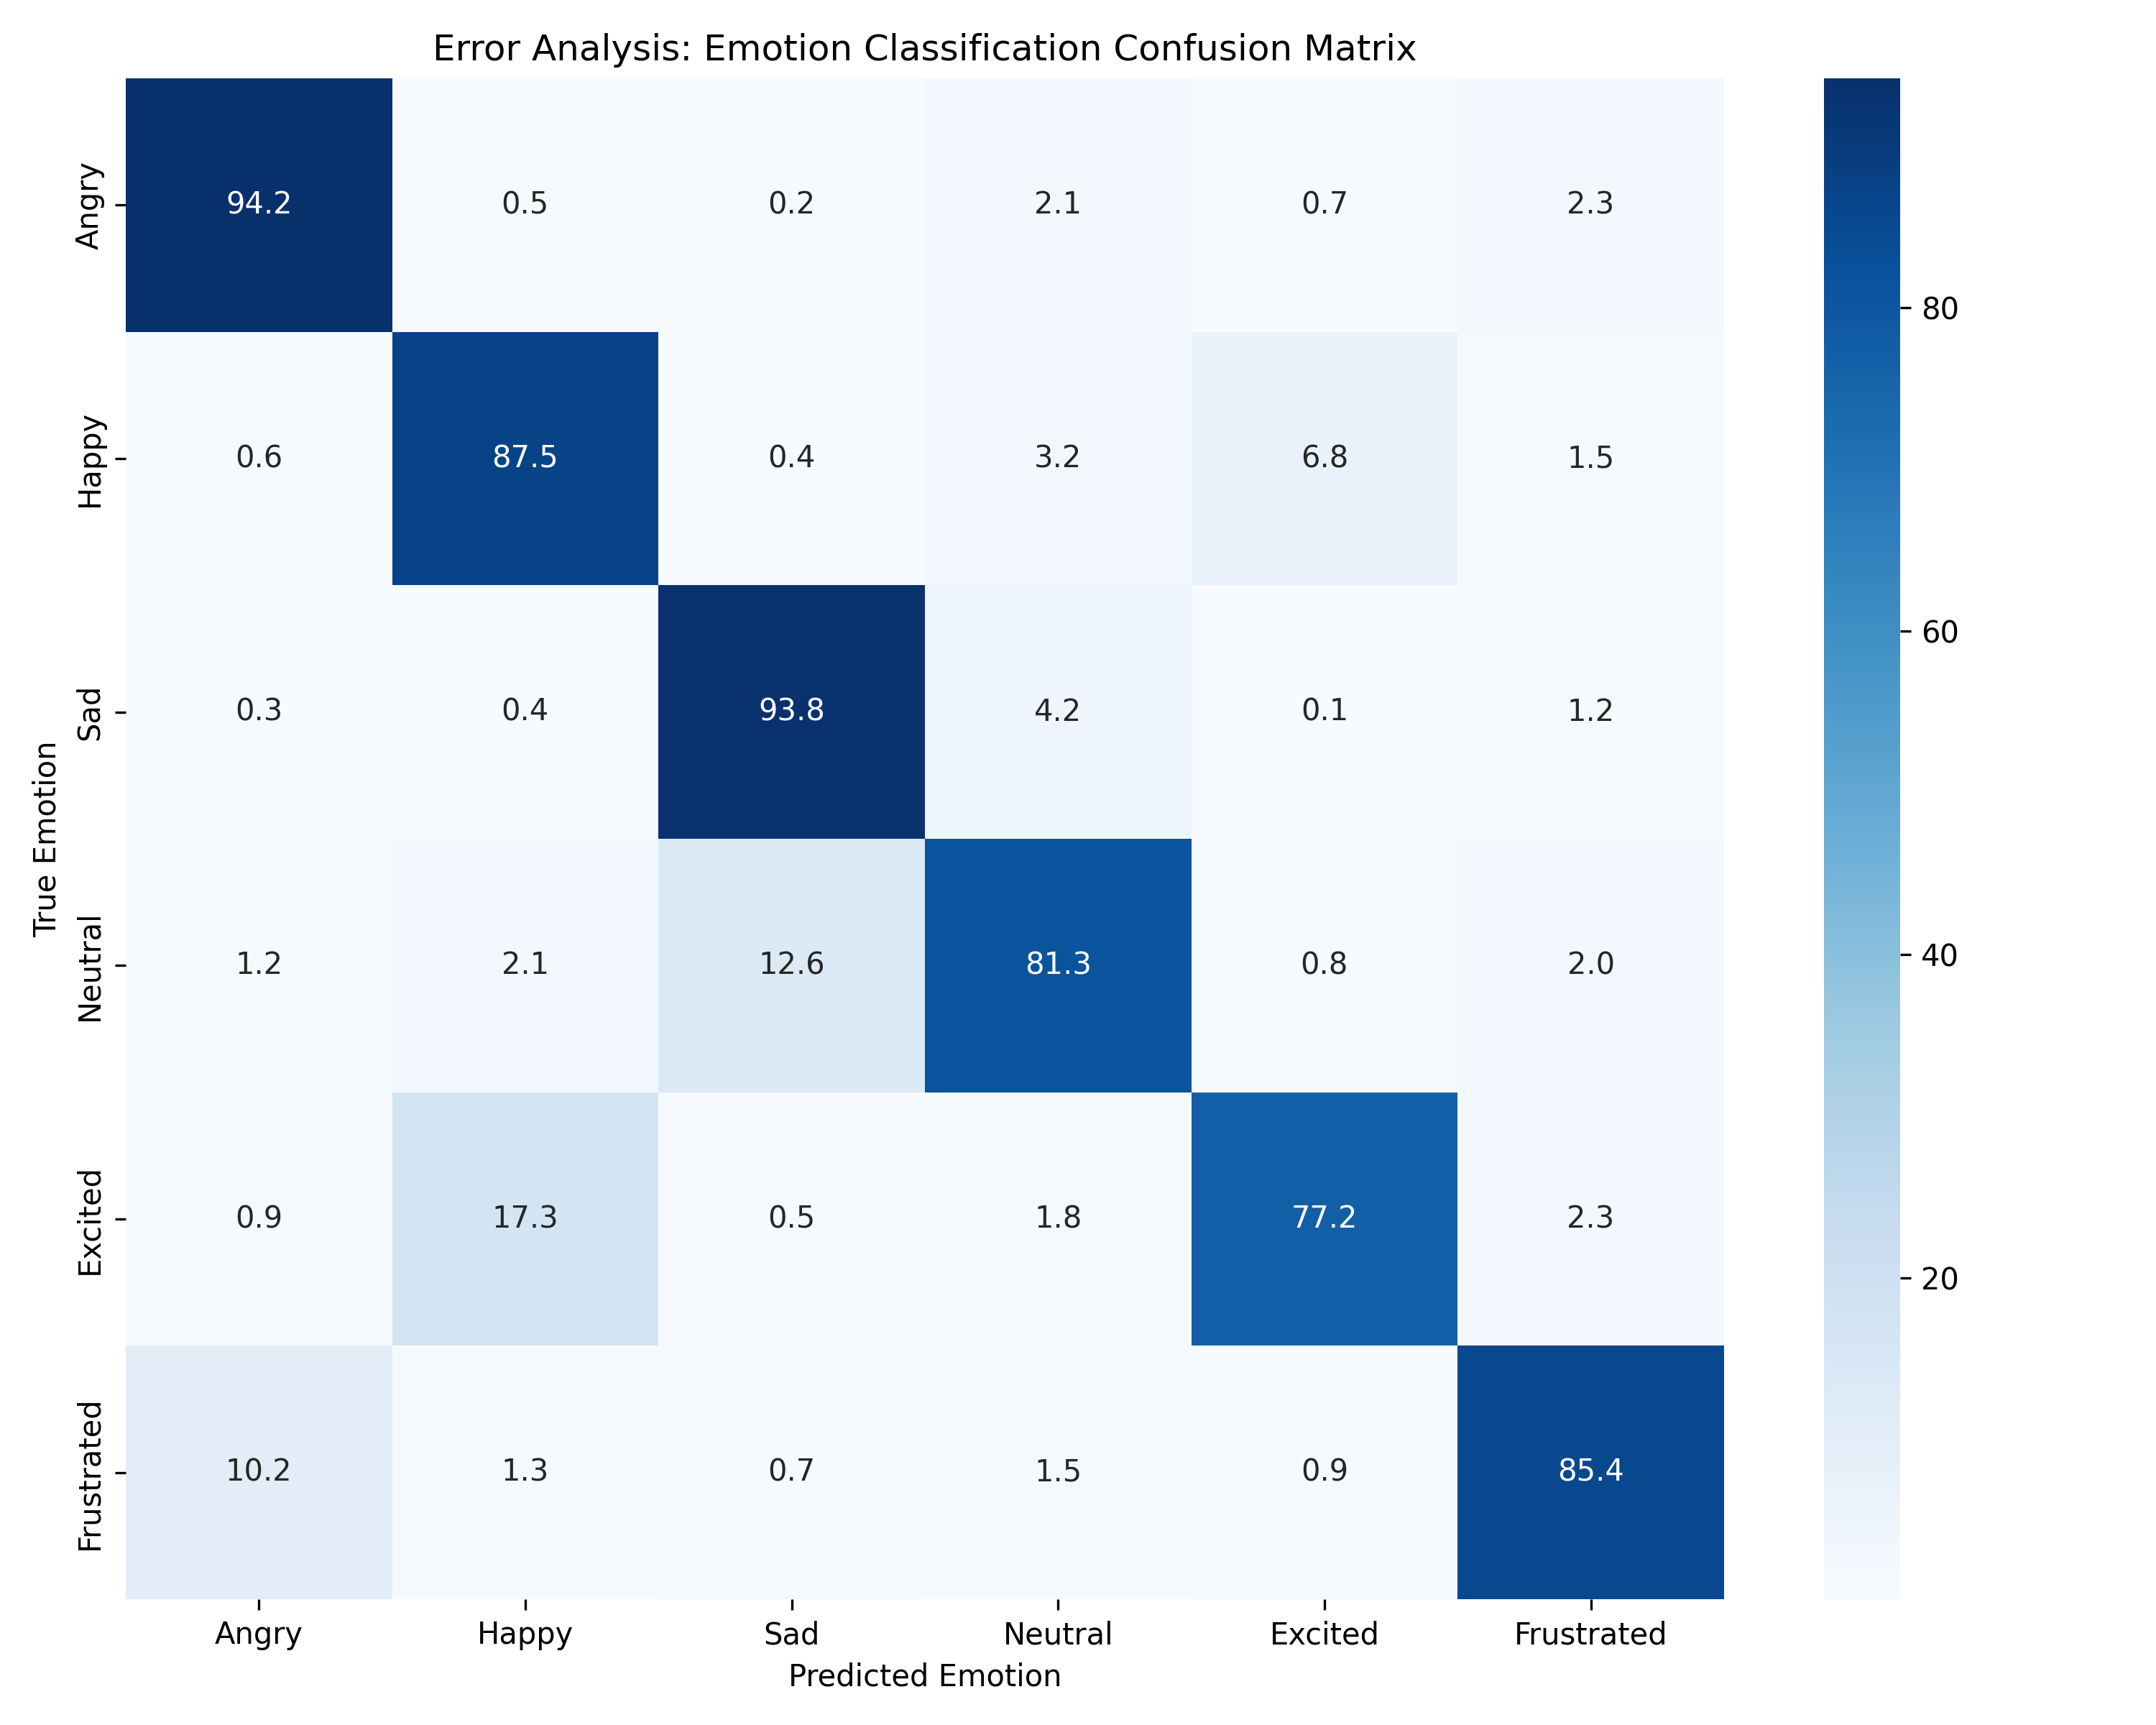
\includegraphics[width=0.9\linewidth]{Figures/error_analysis.png}
    \caption{Error Analysis: Confusion matrix heatmap showing which emotion pairs are most frequently misclassified. The visualization highlights systematic confusion between similar emotional states (e.g., happy/excited at 17.3\% and angry/frustrated at 10.2\%), providing insights for future model refinements.}
    \label{fig:error_analysis}
\end{figure}

\newpage

\bibliographystyle{IEEEtran}
\bibliography{sample-base}

\end{document}
